%%
%% This is file `skeleton.tex',
%% generated with the docstrip utility.
%%
%% The original source files were:
%%
%% nuthesis.dtx  (with options: `skeleton')
%% 
%\RequirePackage{lineno}
%%
%% For common degrees, you can use the class options:
%% phd, edd, ms, ma
%% phd is the default
\documentclass[print]{nuthesis}

%% Needed to typset the math in this sample
\usepackage{amsmath}
\usepackage{amsfonts}
%% Let's use a different font
\usepackage[sc,osf]{mathpazo}

%% Makes things look better
\usepackage{microtype}

%% Makes things look better
\usepackage{booktabs}
%% Gives us extra list environments
\usepackage{paralist}

%% Be able to include graphicsx
\usepackage{graphicx}
\usepackage{caption}
%\usepackage{subcaption}

%% I like darker colors
\usepackage{color}
\definecolor{dark-red}{rgb}{0.6,0,0}
\definecolor{dark-green}{rgb}{0,0.6,0}
\definecolor{dark-blue}{rgb}{0,0,0.6}

%% Needed by memoir to fix things with hyperref
\usepackage{memhfixc}



\begin{document}
%% Start formatting the first few special pages
%% frontmatter is needed to set the page numbering correctly
\frontmatter
%\pagenumbering{}
\title{A Measurement of the $W\gamma$ Cross Section at $\sqrt{s}=8$~TeV in $pp$ Collisions with the CMS Detector}
\author{Ekaterina Avdeeva}
\adviser{Professor Ilya Kravchenko}
\adviserAbstract{Someone}
\major{Physics \& Astronomy}
\degreemonth{May}
\degreeyear{2017}
%%
%% For most people the defaults will be correct, so they are commented
%% out. To manually set these, just uncomment and make the needed
%% changes.
%% \college{Your college}
%% \city{Your City}
%%
%% For most people the following can be changed with a class
%% option. To manually set these, just uncomment the following and
%% make the needed changes.
%% \doctype{Thesis or Dissertation}
%% \degree{Your degree}
%% \degreeabbreviation{Your degree abbr.}
%%
%% Now that we know everything we need, we can generate the title page
%% itself.
%%
\maketitle
%%
%% You have a maximum of 350 words for your abstract, which includes
%% your title, name, etc.
%%
%% Required
\begin{abstract}
 Abstract goes here.
\end{abstract}

%% Optional
%% \begin{copyrightpage}
%% \end{copyrightpage}

%% Optional
%% \begin{dedication}
%% \end{dedication}

%% Optional
%% \begin{acknowledgments}
%% \end{acknowledgments}

%% Optional
%% \begin{grantinfo}
%% \end{grantinfo}
%% The ToC is required
%% Uncomment these if need be

%% The ToC is required
\tableofcontents
%% Uncomment these if need be
%\listoffigures
%\listoftables
%%
%% ``Real'' beginning of the document.
%% mainmatter is needed to set the page numbering correctly
%%   mainmatter is needed after the ToC, (LoF, and LoT) to set the
%%   page numbering correctly for the main body
\mainmatter

%% Thesis goes here

%\chapter{My Thesis}
\section{Introduction}
\label{sec:intro}


Elementary particle physics describes our world in terms of its smallest constituents, fundamental particles, and their interactions. Going from larger to smaller scales, substances around us consist of molecules, molecules consist of atoms, in an atom, there is a nucleus made of neutrons and protons and some number of electrons occupying their orbits around the nucleus. Protons and neutrons have a structure while an electron is not known to have any structure, therefore, an electron is an example of a particle which is considered to be fundamental.\\

Interactions of elementary particles are described by quantum field theories which incorporate principles of the quantum mechanics and the special theory of relativity. The set of such theories, including quantum elecrtrodynamics (QED), quantum chromodynamics (QCD) and the theory of weak interactions is called the Standard Model (SM). It has been proven to be an accurate description of interactions of elementary particles observed by now.\\ 

However, there are several experimental observations which are not described by the SM such as gravity, dark matter, dark energy, matter/antimatter asymmetry and others. Therefore, the SM is not the complete theory of particle interactions. There are several SM extensions offered by theorists as well as radically new theories waiting for the experimental confirmation or disproof. \\

Some SM extensions and new theories predict the existence of heavy particles mass of which possibly lies beyond experimentally reachable energies. The search of these particles is one of the prioritized directions in particle physics. One source of highly energetic elementary particles is cosmic rays. The most energetic particles ever observed came from this source. However, cosmic rays are totally uncontrollable and such highly energetic particles are rare. If we want to produce a large number of particles in a given energy range, we need to use a particle accelerator. A large amount of data allows experimentalists to perform a statistical analysis and increase the probability to find a new particle if it exists.\\

Symmetric colliding beams is the most effective way to produce as heavy particles as possible given the energies of the colliding particles. Comparing to experiments of colliding a single beam to a fixed target, in case of a symmetric collision the total momentum of two colliding particles is zero and, therefore, much larger fraction of energy can transfer to a mass of a new particle.  The Large Hadron Collider (LHC) is such a collider with the highest energy in the world ever built. It can produce the most massive particles to probe physics beyond the SM. It collides two proton ($pp$) beams, two lead ion beams ($Pb-Pb$) or a proton beam to a lead ion beam ($p-Pb$). The design energies for a colliding proton and a colliding lead ion at LHC are~7~TeV and~522~TeV respectively. \\

Compact Muon Solenoid (CMS) is one of two general-purpose detectors at the LHC. It is placed at one of six collision points. CMS has a wide physics program including searches for the beyond SM (BSM) physics as well as the precision measurements of the SM parameters themselves.\\

%In this dissertation the analysis of $pp\rightarrow W\gamma + X$  processes using  leptonic decays of $W\to \ell\nu$ where $\ell = e, \mu$ is reported. The $W\gamma$ productions with leptonic $W$ decays can go through one of the following three processes: initial state radiation where a photon is produced from one of the incoming partons, final state radiation where a photon is radiated off the charged lepton from the $W$ boson decay, and finally when a photon is produced via the triple gauge coupling (TGC) where a photon is emitted from the $W$ boson. \\ 

%To search for the deviations from the SM, one would search for an anomalous TGC which would be indicated by the enhance of the TGC production over the SM prediction. \\

The total and the differential cross section with respect to the photon transverse momentum ($P_T^\gamma$) has been measured. The $P_T^{\gamma}$ is sensitive to the potential anomalous TGC (aTGC) in the high $P_T^{\gamma}$ region. The disagreement between the measured and theoretically predicted differential cross section at the higher $P_T^{\gamma}$ end would be an indication of the possible presence of the aTGC. \\

The rest of this chapter gives general introductory information about the SM while chapter \ref{sec:WgAbout} concentrates on the theory of the SM and BSM $W\gamma$ production and also discusses previous measurements of this process. Chapter \ref{sec:Exp} describes LHC and CMS in more details. Chapter \ref{sec:alignment} explaines on specific aspect of the CMS operation which is the tracker alignment. Finally, chapter \ref{sec:AN_WgMeas} describes the details of the measurement of this dissertation and reports the results.\\ 



%\subsection{Fundamental Particles and Interactions}
\label{sec:Intro_FundParticles}

The SM describes interactions of elementary particles. There are four fundamental interactions: electromagnetic, strong, weak and gravitational. The gravity is not included into the SM but its effect on particles is negligible compared to the other forces which makes it possible to develop a theory of the particle physics and conduct experiments even without having the gravity included into the model.\\ 

All fundamental elementary particles in the SM can be split into three categories by their spins. There are fermions which possess spin s=1/2, there are gauge bosons which are vector particles (s=1) and there is the Higgs boson which is a scalar particle (s=0). \\

The fermions are arranged into three generations, each generation consists of a quark with charge Q=$+$2/3(up, charm, and top quarks), a quark with Q=$-$1/3 (down, strange, and bottom quarks), a charged lepton with Q=$-$1 (electron, muon, and tau-lepton) and a neutrino (electron, muon, and tau neutrinos) which is electrically neutral. Each quark can carry any of three colors: red, blue, or green. Additionally, each fermion has its antiparticle. Therefore, the total number of fundamental fermions is $(6 ($leptons$)+6 ($quarks$) \cdot 3 ($colors$) ) \cdot 2 ($to~include~antiparticles$) = 48$.\\ 

Corresponding particles in different generations have the same charges, spins and interaction properties but masses of particles increase with a generation. These mass differences lead to different decay properties because a particle A can decay to particles B and C only if their masses relate as $m_A > m_B + m_C$. Thus, an electron is a stable particle, a muon decays as $\mu^- \rightarrow e^- + \bar{\nu_e} + \nu_\mu$, a tau-lepton, as the heaviest charged lepton, has the largest number of decay channels amongst the charged leptons: $\tau^- \rightarrow \mu^- + \bar{\nu_\mu} + \nu_\tau$, $\tau^- \rightarrow e^- + \bar{\nu_e} + \nu_\tau$,  $\tau^- \rightarrow \nu_\tau +$ quarks. \\

In addition to fermions, the SM includes gauge bosons which are interaction mediators. They are called mediators because fermions interact with each other by exchanging them. For example, two charged fermions can interact with each other by exchanging a photon. Such interaction is called electromagnetic interaction and a photon is a mediator for the electromagnetic interaction. Similarly, a gluon is a mediator for strong interactions, and W$^{\pm}$ and Z$^0$ bosons are mediators for weak interactions. W$^{\pm}$ and Z$^0$ bosons are massive while a photon and a gluon are massless particles. \\

The last SM particle is the Higgs boson. The Higgs boson is a scalar neutral particle which is playing a critical role in the electroweak symmetry breaking. The Higgs mechanism explains how $W$ and $Z$ bosons become massive particles.\\

All the particles are summarized in Fig.~\ref{fig:SMtable}. These and only these fundamental particles and their antiparticles have been discovered by now. However, there are many composite particles which are called hadrons. Hadrons can consist of three quarks (baryons), quark and antiquark (meson), or three antiquarks (antibaryons). Hadrons always possess an integer charge.\\

Most of the particles are short-lived and decay within microseconds. The only stable particles are protons and antiprotons, electrons and positrons, neutrinos and antineutrinos, photons, and, in some sense, gluons. However, if a particle cannot decay, it does not mean that it would live forever. There are many different kinds of reactions in which particles can disappear. Antiprotons and positrons would immediately annihilate with protons and electrons, photons can be absorbed by charged particles, electrons and protons can scatter to produce neutrons and neutrinos and many other reactions are possible.\\ 

In this dissertation, the study of $pp\rightarrow W\gamma + X$ process where the $W$ decays as $W\to \ell\nu$ where $\ell = e, \mu$ is reported. The $W\gamma$ production with leptonic $W$ decays proceeds through one of the following three processes: the initial state radiation where a photon is emitted from one of the incoming partons, the final state radiation where a photon is radiated off the charged lepton from the $W$ boson decay, and, finally, the triple gauge coupling (TGC) where a photon is emitted from the $W$ boson. Many BSM theories predict an enchancement of the TGC production over the SM value and, therefore, the experimental search for such an enchancement is a good test for such theories.\\ 
%The total and the differential cross section with respect to the photon transverse momentum ($P_T^\gamma$) has been measured. The $P_T^{\gamma}$ is sensitive to the potential anomalous TGC (aTGC) in the high $P_T^{\gamma}$ region. The disagreement between the measured and theoretically predicted differential cross section at the higher $P_T^{\gamma}$ end would be an indication of the possible presence of the aTGC.

%In this dissertation a process is studied where quark and antiquark interact to produce a $W$ boson which then decay as $W^\pm \rightarrow e^\pm \nu_e(\bar{\nu_e})$ or $W^\pm \rightarrow \mu^\pm \nu_\mu(\bar{\nu_\mu}) $. A photon is radiated off a quark or antiquark, a charged lepton or a $W$ boson. The most interesting mechanism out of three is a radiation from a $W$ boson because this is the triple gauge coupling where we potentially can have a new physics. 

Therefore, the focus of this study is an interaction between a photon and a $W$ boson however many other SM particles are relevant too. Thus, a charged lepton and a neutrino appear as the final state particles, a quark and an antiquark appear as initial state particles and all fundamental particles except the Higgs boson participate in various background processes. Subsections \ref{sec:Intro_Electroweak}-\ref{sec:Intro_ppCollisions}, chapter \ref{sec:WgAbout} and \cite{ref_Griffiths} describe particle interactions in more details.\\


\begin{figure}[htb]
  \begin{center}
    {\includegraphics[width=0.90\textwidth]{../figs/Intro/StandardModel.png}}
    \caption{Standard Model Particles and Interations. Source of the figure: \cite{ref_fig_SM}.}
    \label{fig:SMtable}
  \end{center}
\end{figure}






%\subsection{Electroweak Interactions}
\label{sec:Intro_Electroweak}



% The style needs to be improved. Some places contain very chopped language.
% Consider this passage, way too “chopped”:
% > Elementary processes with W and Z bosons are shown in Fig. 3. An electric charge must be
% > conserved at any vertex. Therefore, if a charged lepton enters and radiates a W boson, a
% > neutrino or antineutrino escapes (top left in Fig. 3). That is how a W boson interacts with a
% > charged lepton and a neutrino. A lepton flavor number is always conserved in this interaction (Tab. 1).
%Consider using math mode for single character particle names, such as $c$ or $d$, to make them distinct in the text.

All electrically charged particles participate in electromagnetic interactions. Photon, the mediator of the electromagnetic interactions, is a spin-one electrically neutral massless particle. All electromagnetic interactions can be reduced to one elementary process (Fig. \ref{fig:feynmEM}, left). This process reads: an electron enters, radiates or absorbs a photon, and escapes. Although there is an electron is drawn in this figure, it can be any other charged particle as well. Such elementary process itself is forbidden by the energy conservation law but this element is a base of actual process (for example, Fig. \ref{fig:feynmEM}, middle and right). Such graphical representations of the particle physics processes are called Feynman diagrams.\\ 

\begin{figure}[htb]
  \begin{center}
    {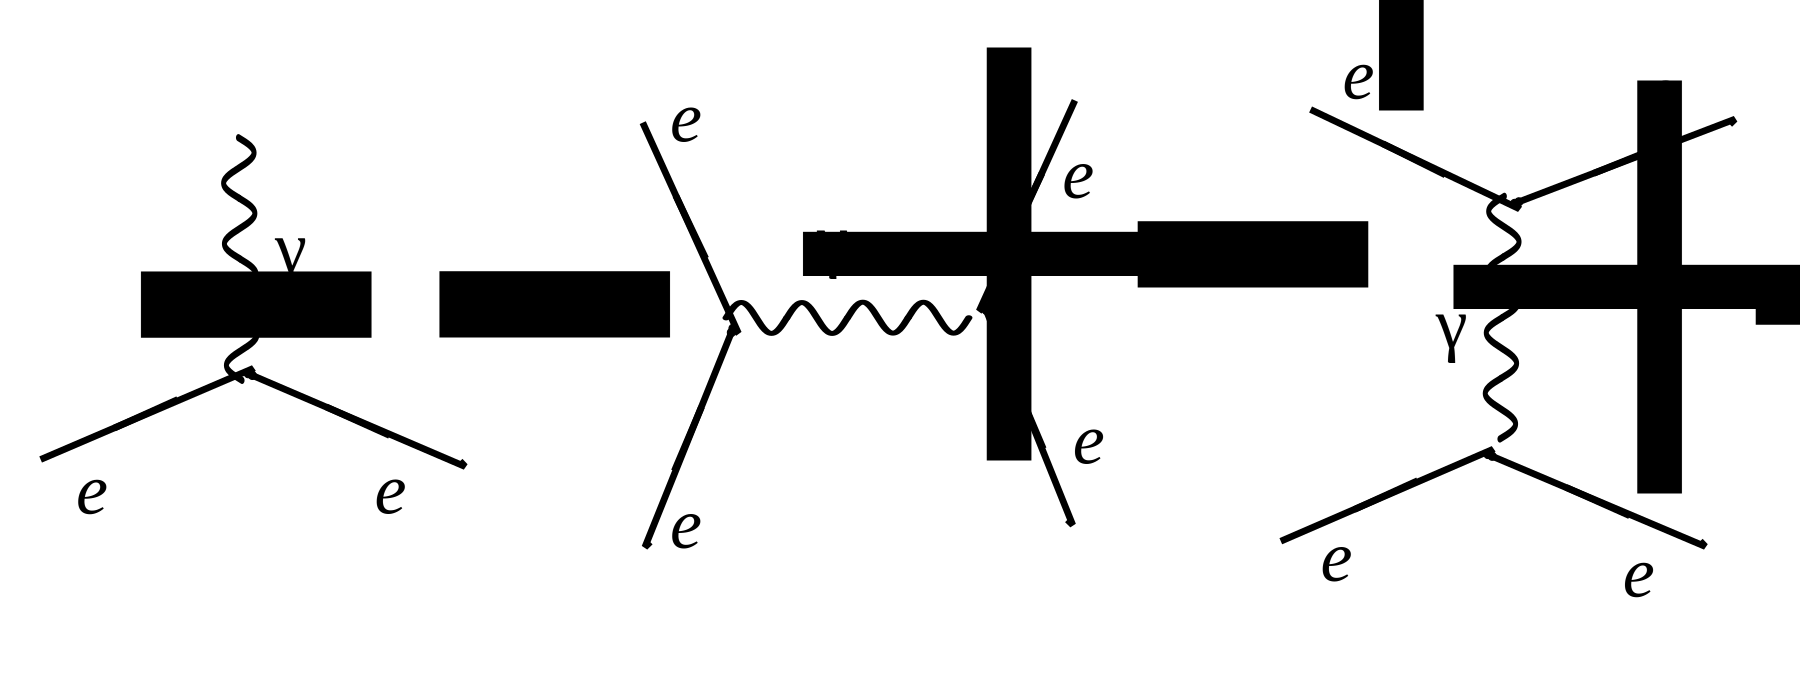
\includegraphics[width=0.90\textwidth]{../figs/Intro/feynmEM.png}}
    \caption{Electromagnetic interations}
    \label{fig:feynmEM}
  \end{center}
\end{figure}

\begin{figure}[htb]
  \begin{center}
    {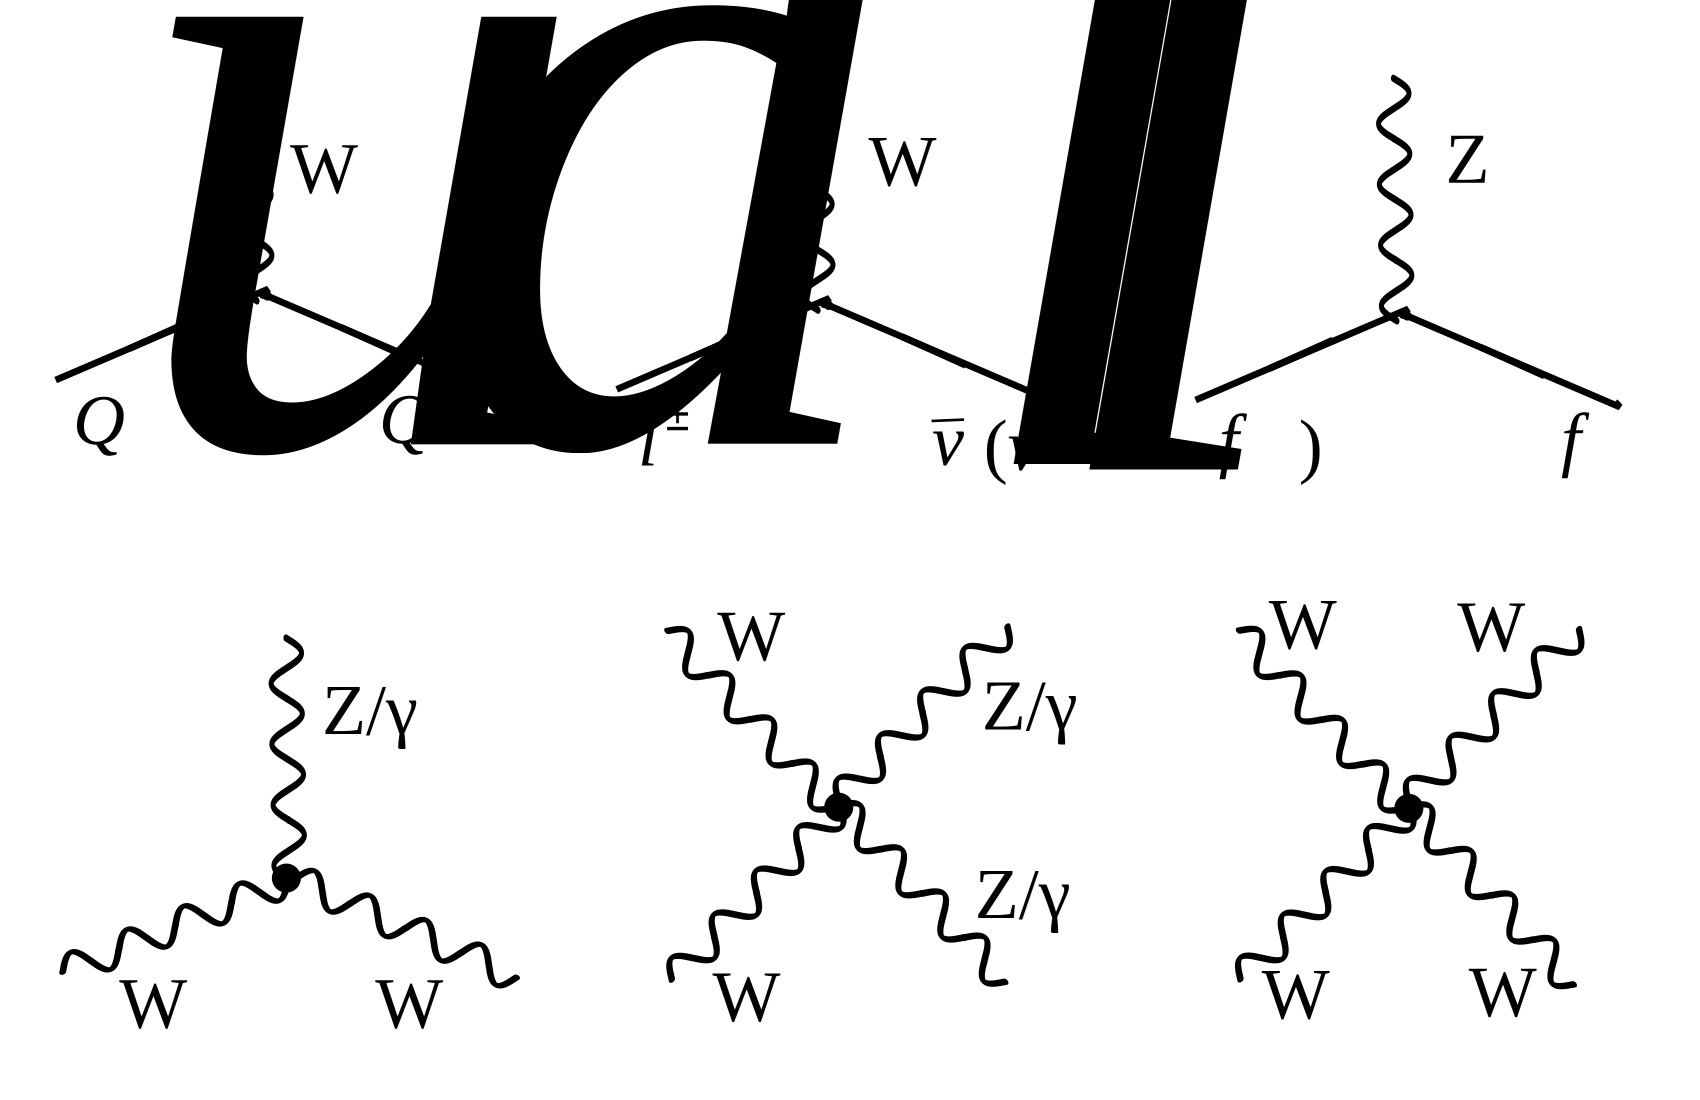
\includegraphics[width=0.90\textwidth]{../figs/Intro/feynmW.png}}
    \caption{Weak interations}
    \label{fig:feynmW}
  \end{center}
\end{figure}


As for the weak interactions, there are two kinds of them: neutral (mediated by a Z boson) and charged (mediated by a W$\pm$ boson). Elementary processes with W and Z bosons are shown in Fig. \ref{fig:feynmW}. Because the electric charge must be conserved at any vertex, a particle radiating or absorbing a W boson converts to a different particle. Thus, a charged lepton converts to a neutrino (or vice versa) as shown in Fig. \ref{fig:feynmW}, top left. A lepton flavor number is always conserved in such interactions (lepton flavor numbers assigned to different lepton are summarized in Tab. \ref{tab:LeptonFlavorNumber}), thus an electron always converts to an electron neutrino, a muon always converts to a muon neutrino etc.\\

 \begin{table}[h]
  \begin{center}
  \caption{ Lepton Flavor Number}
  \begin{tabular}{|c|c|c|c|}
     particles & $L_e$ & $L_{\mu}$ & $L_{\tau}$ \\ \hline
     $e^-,\nu_e$ &  +1  &  0  &  0  \\ \hline 
     $e^+, \bar{\nu_e}$ &  -1  &  0  &  0  \\ \hline 
     $\mu^-,\nu_{\mu}$ &  0  &  +1  &  0  \\ \hline 
     $\mu^+, \bar{\nu_{\mu}}$ &  0  &  -1  &  0  \\ \hline 
     $\tau^-,\nu_{\tau}$ &  0  &  0  &  +1  \\ \hline 
     $\tau^+, \bar{\nu_{\tau}}$ &  0  &  0  &  -1  \\ \hline 
  \end{tabular}
  \label{tab:LeptonFlavorNumber}
  \end{center}
 \end{table}

From top middle diagram in Fig. \ref{fig:feynmW} we see that if a quark with Q=-1/3 enters, then a quark with Q=+2/3 escapes and, therefore, the flavor of the quark has changed. The charged weak interaction is the only interaction which changes a quark flavor. The probability of each of three quarks with Q=+2/3 to be born is determined by the Cabibbo–Kobayashi–Maskawa matrix and is the highest for the quark of the same generation as an initial state quark (in this particular case, $d$ is the initial state quark and $u$ has the highest probability to be produced after an interaction with a W boson but $c$ and $t$ can also be produced if there is enough energy).\\

An elementary process of a neutral weak interactions is an emission of a Z boson off a fermion line (right top diagram in Fig. \ref{fig:feynmW}). An electron is shown here as an example however it also could be any lepton, antilepton, quark or antiquark. Diagrams with a Z boson are very similar to ones with a photon except a photon can only be radiated off a charged particle but a Z boson can also be radiated off a neutrino or antineutrino.\\

The bottom diagrams in Fig. \ref{fig:feynmW} are gauge coupling diagrams. Gauge couplings include self-coupling of a W boson, its interaction with Z boson and its electromagnetic radiation of a photon. WWZ, WW$\gamma$, WWZZ, WWZ$\gamma$, WW$\gamma\gamma$ and WWWW vertices are all possible in the SM.\\

Electromagnetic and weak interactions are unified by the electroweak theory. This theory considers these two forces as different manifestations of the electroweak force. While both forces can be described by very similar formalism, there is also a big difference between them: weak interactions are mediated by heavy bosons ($M_W=80$ GeV, $M_Z=91$ GeV) while electromagnetic interactions are described by a massless photon. \\

To explain this phenomenon, the Higgs mechanism was introduced. The mechanism predicted an existence of an additional boson - the Higgs boson. The Higgs boson was a missing piece of the SM for many years and was finally discovered in 2012 at the LHC by ATLAS and CMS collaborations through the processes shown in Fig.\ref{fig:higgsProduction}.\\ 

\begin{figure}[htb]
  \begin{center}
    {\includegraphics[width=0.95\textwidth]{../figs/Intro/FeynmanHiggs.png}}
    \caption{Higgs production and decay}
    \label{fig:higgsProduction}
  \end{center}
\end{figure}

The measurement in this dissertation is an electroweak measurement because the process involves a W boson. It includes an interaction of a W boson with leptons and quarks as well as the gauge coupling WW$\gamma$. Thus, the measurement is a good test of the SM electroweak theory.\\ 




%\subsection{The Higgs Boson}
\label{Intro_Higgs}

% BAD SECTION
% NEEDS TO BE SIGNIFICANTLY REWORKED

\begin{figure}[htb]
  \begin{center}
    {\includegraphics[width=0.95\textwidth]{../figs/Intro/FeynmanHiggs.png}}
    \caption{Higgs production and decay}
    \label{fig:higgsProduction}
  \end{center}
\end{figure}

%  I feel that there is a number of imprecise statements here that need to be corrected. Here are examples.
%   (A side note: quant is not what you mean, check the dictionary. You want to say “quantum”)
%   I would not say that the Higgs boson is a quantum of the Higgs field. The Higgs field is a doublet of complex fields, i.e. it has four components. According to wikipedia wording, for example, “it is a quantum excitation of one of the four components of the Higgs field. "
% This part: "discovered by ATLAS and CMS collaborations in the reaction shown in Fig. 4 in γγ and ZZ decay channels”
% The diagram in Fig. 4 is not appropriate for ZZ.
% "the same approach can be used to introduced masses of all elementary particles.” - but what about neutrinos? I am not sure if our favorite explanation of neutrino masses is the Higgs.
% It is not intuitive to me that larger mass means stronger interaction with the Higgs field,
% I am not sure why you say that.
% "that is how is gets its inertia”: consider rephrasing.









%\subsection{Strong Interactions}
\label{sec:Intro_QCD}

\begin{figure}[htb]
  \begin{center}
    {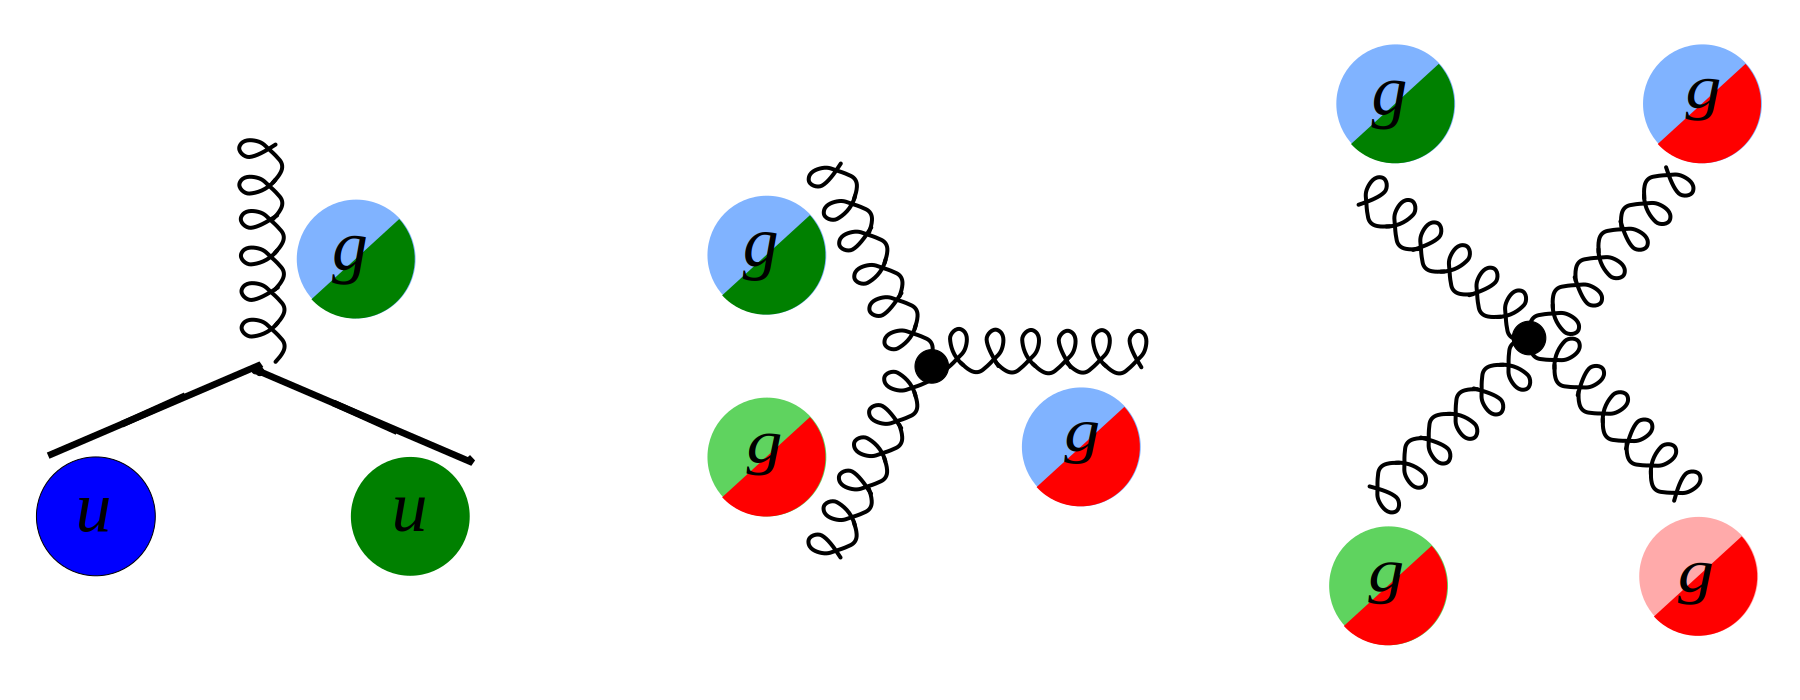
\includegraphics[width=0.90\textwidth]{../figs/Intro/feynmStrong.png}}
    \caption{Strong interations}
    \label{fig:feynmStrong}
  \end{center}
\end{figure}

 %  Again, I do not see a connective narrative. Paragraphs are sets of loosely connected sentences, the section is a set of loosely connected paragraphs. Needs imporvement.
% Somewhat reverse flow of ideas, example:
% > There are eight types of gluons corresponding to different color-anticolor combinations.
% > Gluons are spin-one massless electrically neutral particles.
% First, you should say what gluons ARE, and then you can say what types of gluons exist.
% > Gluons possess color charges, therefore, they can self-interact.
% The emphasis of this statement is that gluons possess color charges, which is odd because you already mentioned it some number of times above (which adds to the feeling of reverse flow).
% Instead, the emphasis of the sentence should be that they can self-inteact.
% Some incorrect information, for example:
% "it becomes larger as the distance becomes smaller” about the coupling constant: it becomes smaller at smaller distances, larger at larger distances.

The third fundamental force after the electromagnetic and weak ones is the strong force. The strong force is responsible for glueing protons and neutrons together in the nuclea as well as for forming protons and neutrons themselves. The strong interactions are performed by exchanging gluons which are spin-one massless electrically neutral particles.  \\

The elementary strong processes are shown in Fig. \ref{fig:feynmStrong}. There are three elementary processes: qqg, ggg and gggg, all are involving particles with color charges. Thus, gluons couple to quarks and self-couple. Color charges must be conserved at each elementary process of the strong interaction. And because quarks can possess three colors, there are eight types of gluons to cover all possible color exchanges. \\

The coupling constant of the strong interaction depends on a distance between interacting particles: it becomes larger as the distance becomes larger. This property leads to two consequences specific to the strong force: the confinement and the asymptotic freedom.\\

The confinement is the property of quarks to always stay in the colorly neutral combinations (hadrons), it forbids the existence of free quarks. A combination becomes colorly neutral when there is the same amount of color and anticolor or if there is the same amount of each of the three colors.  There are two types of hadros: mesons (comprised of a quark and antiquarks with the opposite color charges) and baryons (comprised of three quarks: a red, a green and a blue one). The widely known particles a proton and a neutron are baryons.\\

The asymptotic freedom means that when quarks are very close to each other they almost do not interact with each other and therefore they are free. When the distance between quarks is low which corresponds to high energy, and thus the coupling constant $1/\alpha_s \ll 1$ is low, the strong interactions can be described by a perturbative quantum field theory which is called quantum chromodynamics (QCD).\\

The W$\gamma$ process being measured in this dissertation is not intended to test QCD, but a good understanding of QCD is essential for performing this measurement. First of all, QCD describes the dynamics of quarks and gluons within colliding protons and predicts probabilities of one or another quark-antiquark pair to annihilate. Secondly, the QCD corrections to the Feynman diagrams of the process are large and has to be taken into account in producing simulation. Possible QCD correction include quark-gluon loops at any of three quark lines as well as exchanges of gluons between different quark lines.\\
 

%\subsection{Physcis of Proton-Proton Collisions}
Physcis of Proton-Proton Collisions

%\section{Open Questions of the Standard Model}


While the SM is an accurate description of all particle physics experimental results, there are certain phenomena which are not included into the SM. In this subsection we discuss some of them.

The gravitational interactions do not fit into the SM. It is the open question whether the quantum theory of gravity is possible and whether there is a mediator of the gravitational interactions. Also, it is not known why the gravitational force is so much weaker than the other forces. One possible explanation comes from a theory which predicts extra spatial dimensions beyond the three we experience (e.g. the string theory). In this case, it is possible that the gravitational force is shared with other dimensions and only a fraction is available in our three dimensions.

Another mystery of the universe is its composition: it is known from the studies of the gravitational effects that our universe consists of dark energy by 68\%, of dark matter by 27\% and of baryon matter only by 5\%~\cite{ref_NASA}. The dark energy resists the gravitational attraction and accelerates the expansion of the universe, and is not detectable by any effects except gravitational. The understanding of dark energy is a question of general relativity rather than particle physics. The dark matter, however, likely consists of particles and therefore is a subject of particle physics. It does not radiate and that is why it cannot be detected by telescopes. The nature of the dark matter is not known but its constituents must be very stable to remain since the Big Bang. The theory of the supersymmetry which is unifying fundamental particles and mediators predicts many of new heavy particles and the lightest supersymmetric particle, the neutralino, is a good candidate for dark matter.

One more open question is the reason for the matter/antimatter asymmetry. Matter and antimatter should have been created in the same amount at the moment of the Big Bang. Most of it has annihilated but because of asymmetry, there was more matter than antimatter which led to the state of the Universe we observe now. There is a phenomenon of the CP-violation in weak interactions observed and described which predicts the asymmetry at a certain level. However, the effect of the CP-violation is not large enough to account for the observed amount of the matter and, therefore, the total matter/antimatter asymmetry remains unexplained. 

The measurement of the $W\gamma$ production in $pp$ collisions has a goal to both test the SM and search for the BSM physics. We measure a cross section differential in the component of the photon momentum, transverse to the beamline (referred as photon transverse momentum, or $P_T^{\gamma}$). The low $P_T^{\gamma}$ region is not expected to be affected by any new physics and must agree well with the SM predictions while the high $P_T^{\gamma}$ region may indicate an existence of new physics if there is an enhancement over the SM predictions. The excess would be indirect evidence of the BSM particles like supersymmetric particles or additional gauge bosons which could be part of the explanation of the dark matter presence or difference in magnitudes of different interactions. More theoretical details about the SM description of W$\gamma$ process as well as possible BSM physics are given in Ch.~\ref{sec:WgAbout}.    

%Grand unification and super unification


 % 7-20 pages
\subsection{Fundamental Particles and Interactions}
\label{sec:Intro_FundParticles}

The SM describes interactions of elementary particles. There are four fundamental interactions: electromagnetic, strong, weak and gravitational. The gravity is not included into the SM but its effect on particles is negligible compared to the other forces which makes it possible to develop a theory of the particle physics and conduct experiments even without having the gravity included into the model.\\ 

All fundamental elementary particles in the SM can be split into three categories by their spins. There are fermions which possess spin s=1/2, there are gauge bosons which are vector particles (s=1) and there is the Higgs boson which is a scalar particle (s=0). \\

The fermions are arranged into three generations, each generation consists of a quark with charge Q=$+$2/3(up, charm, and top quarks), a quark with Q=$-$1/3 (down, strange, and bottom quarks), a charged lepton with Q=$-$1 (electron, muon, and tau-lepton) and a neutrino (electron, muon, and tau neutrinos) which is electrically neutral. Each quark can carry any of three colors: red, blue, or green. Additionally, each fermion has its antiparticle. Therefore, the total number of fundamental fermions is $(6 ($leptons$)+6 ($quarks$) \cdot 3 ($colors$) ) \cdot 2 ($to~include~antiparticles$) = 48$.\\ 

Corresponding particles in different generations have the same charges, spins and interaction properties but masses of particles increase with a generation. These mass differences lead to different decay properties because a particle A can decay to particles B and C only if their masses relate as $m_A > m_B + m_C$. Thus, an electron is a stable particle, a muon decays as $\mu^- \rightarrow e^- + \bar{\nu_e} + \nu_\mu$, a tau-lepton, as the heaviest charged lepton, has the largest number of decay channels amongst the charged leptons: $\tau^- \rightarrow \mu^- + \bar{\nu_\mu} + \nu_\tau$, $\tau^- \rightarrow e^- + \bar{\nu_e} + \nu_\tau$,  $\tau^- \rightarrow \nu_\tau +$ quarks. \\

In addition to fermions, the SM includes gauge bosons which are interaction mediators. They are called mediators because fermions interact with each other by exchanging them. For example, two charged fermions can interact with each other by exchanging a photon. Such interaction is called electromagnetic interaction and a photon is a mediator for the electromagnetic interaction. Similarly, a gluon is a mediator for strong interactions, and W$^{\pm}$ and Z$^0$ bosons are mediators for weak interactions. W$^{\pm}$ and Z$^0$ bosons are massive while a photon and a gluon are massless particles. \\

The last SM particle is the Higgs boson. The Higgs boson is a scalar neutral particle which is playing a critical role in the electroweak symmetry breaking. The Higgs mechanism explains how $W$ and $Z$ bosons become massive particles.\\

All the particles are summarized in Fig.~\ref{fig:SMtable}. These and only these fundamental particles and their antiparticles have been discovered by now. However, there are many composite particles which are called hadrons. Hadrons can consist of three quarks (baryons), quark and antiquark (meson), or three antiquarks (antibaryons). Hadrons always possess an integer charge.\\

Most of the particles are short-lived and decay within microseconds. The only stable particles are protons and antiprotons, electrons and positrons, neutrinos and antineutrinos, photons, and, in some sense, gluons. However, if a particle cannot decay, it does not mean that it would live forever. There are many different kinds of reactions in which particles can disappear. Antiprotons and positrons would immediately annihilate with protons and electrons, photons can be absorbed by charged particles, electrons and protons can scatter to produce neutrons and neutrinos and many other reactions are possible.\\ 

In this dissertation, the study of $pp\rightarrow W\gamma + X$ process where the $W$ decays as $W\to \ell\nu$ where $\ell = e, \mu$ is reported. The $W\gamma$ production with leptonic $W$ decays proceeds through one of the following three processes: the initial state radiation where a photon is emitted from one of the incoming partons, the final state radiation where a photon is radiated off the charged lepton from the $W$ boson decay, and, finally, the triple gauge coupling (TGC) where a photon is emitted from the $W$ boson. Many BSM theories predict an enchancement of the TGC production over the SM value and, therefore, the experimental search for such an enchancement is a good test for such theories.\\ 
%The total and the differential cross section with respect to the photon transverse momentum ($P_T^\gamma$) has been measured. The $P_T^{\gamma}$ is sensitive to the potential anomalous TGC (aTGC) in the high $P_T^{\gamma}$ region. The disagreement between the measured and theoretically predicted differential cross section at the higher $P_T^{\gamma}$ end would be an indication of the possible presence of the aTGC.

%In this dissertation a process is studied where quark and antiquark interact to produce a $W$ boson which then decay as $W^\pm \rightarrow e^\pm \nu_e(\bar{\nu_e})$ or $W^\pm \rightarrow \mu^\pm \nu_\mu(\bar{\nu_\mu}) $. A photon is radiated off a quark or antiquark, a charged lepton or a $W$ boson. The most interesting mechanism out of three is a radiation from a $W$ boson because this is the triple gauge coupling where we potentially can have a new physics. 

Therefore, the focus of this study is an interaction between a photon and a $W$ boson however many other SM particles are relevant too. Thus, a charged lepton and a neutrino appear as the final state particles, a quark and an antiquark appear as initial state particles and all fundamental particles except the Higgs boson participate in various background processes. Subsections \ref{sec:Intro_Electroweak}-\ref{sec:Intro_ppCollisions}, chapter \ref{sec:WgAbout} and \cite{ref_Griffiths} describe particle interactions in more details.\\


\begin{figure}[htb]
  \begin{center}
    {\includegraphics[width=0.90\textwidth]{../figs/Intro/StandardModel.png}}
    \caption{Standard Model Particles and Interations. Source of the figure: \cite{ref_fig_SM}.}
    \label{fig:SMtable}
  \end{center}
\end{figure}






\subsection{Electroweak Interactions}
\label{sec:Intro_Electroweak}



% The style needs to be improved. Some places contain very chopped language.
% Consider this passage, way too “chopped”:
% > Elementary processes with W and Z bosons are shown in Fig. 3. An electric charge must be
% > conserved at any vertex. Therefore, if a charged lepton enters and radiates a W boson, a
% > neutrino or antineutrino escapes (top left in Fig. 3). That is how a W boson interacts with a
% > charged lepton and a neutrino. A lepton flavor number is always conserved in this interaction (Tab. 1).
%Consider using math mode for single character particle names, such as $c$ or $d$, to make them distinct in the text.

All electrically charged particles participate in electromagnetic interactions. Photon, the mediator of the electromagnetic interactions, is a spin-one electrically neutral massless particle. All electromagnetic interactions can be reduced to one elementary process (Fig. \ref{fig:feynmEM}, left). This process reads: an electron enters, radiates or absorbs a photon, and escapes. Although there is an electron is drawn in this figure, it can be any other charged particle as well. Such elementary process itself is forbidden by the energy conservation law but this element is a base of actual process (for example, Fig. \ref{fig:feynmEM}, middle and right). Such graphical representations of the particle physics processes are called Feynman diagrams.\\ 

\begin{figure}[htb]
  \begin{center}
    {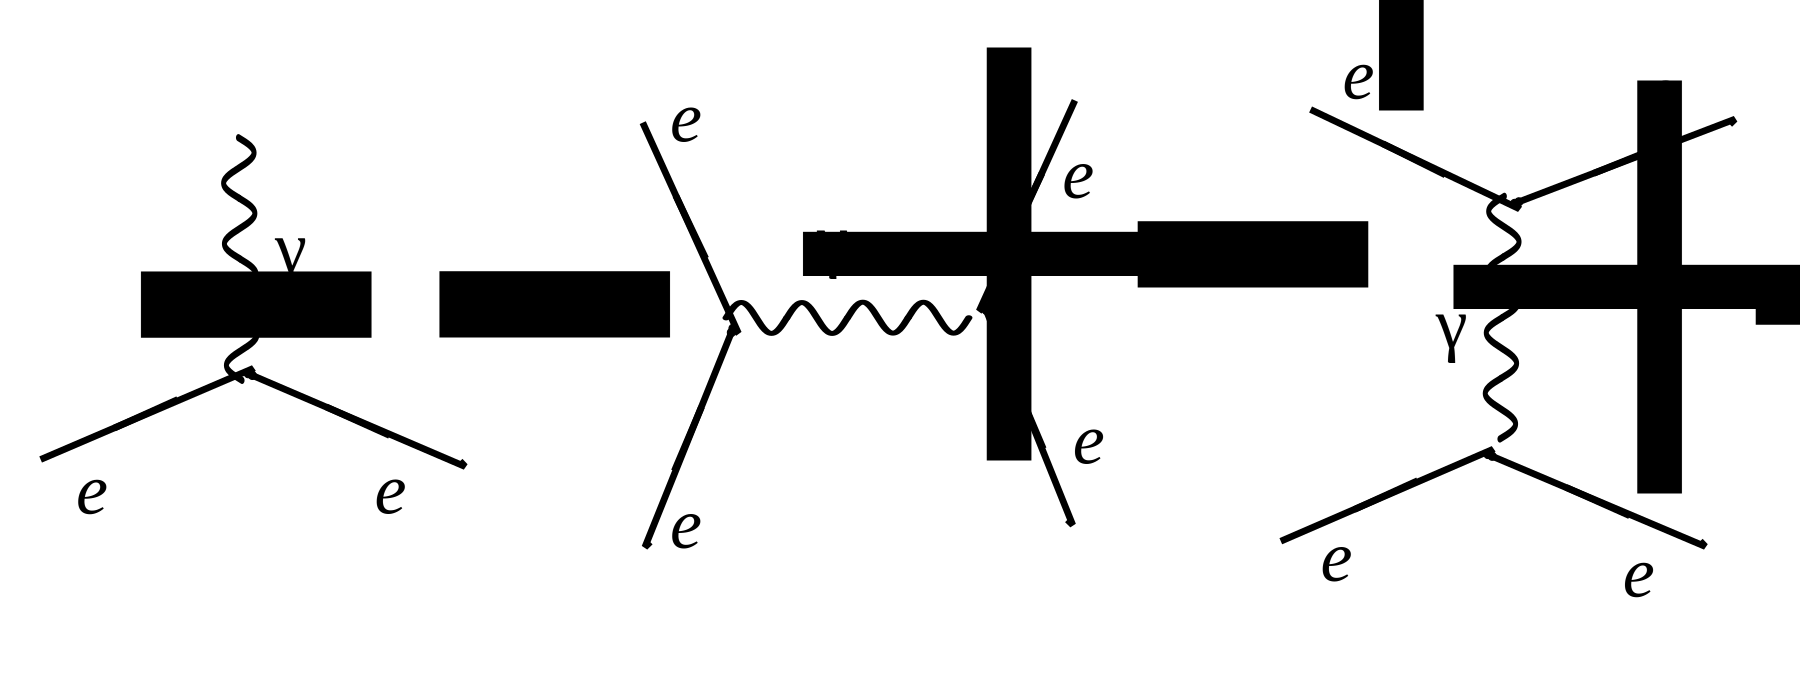
\includegraphics[width=0.90\textwidth]{../figs/Intro/feynmEM.png}}
    \caption{Electromagnetic interations}
    \label{fig:feynmEM}
  \end{center}
\end{figure}

\begin{figure}[htb]
  \begin{center}
    {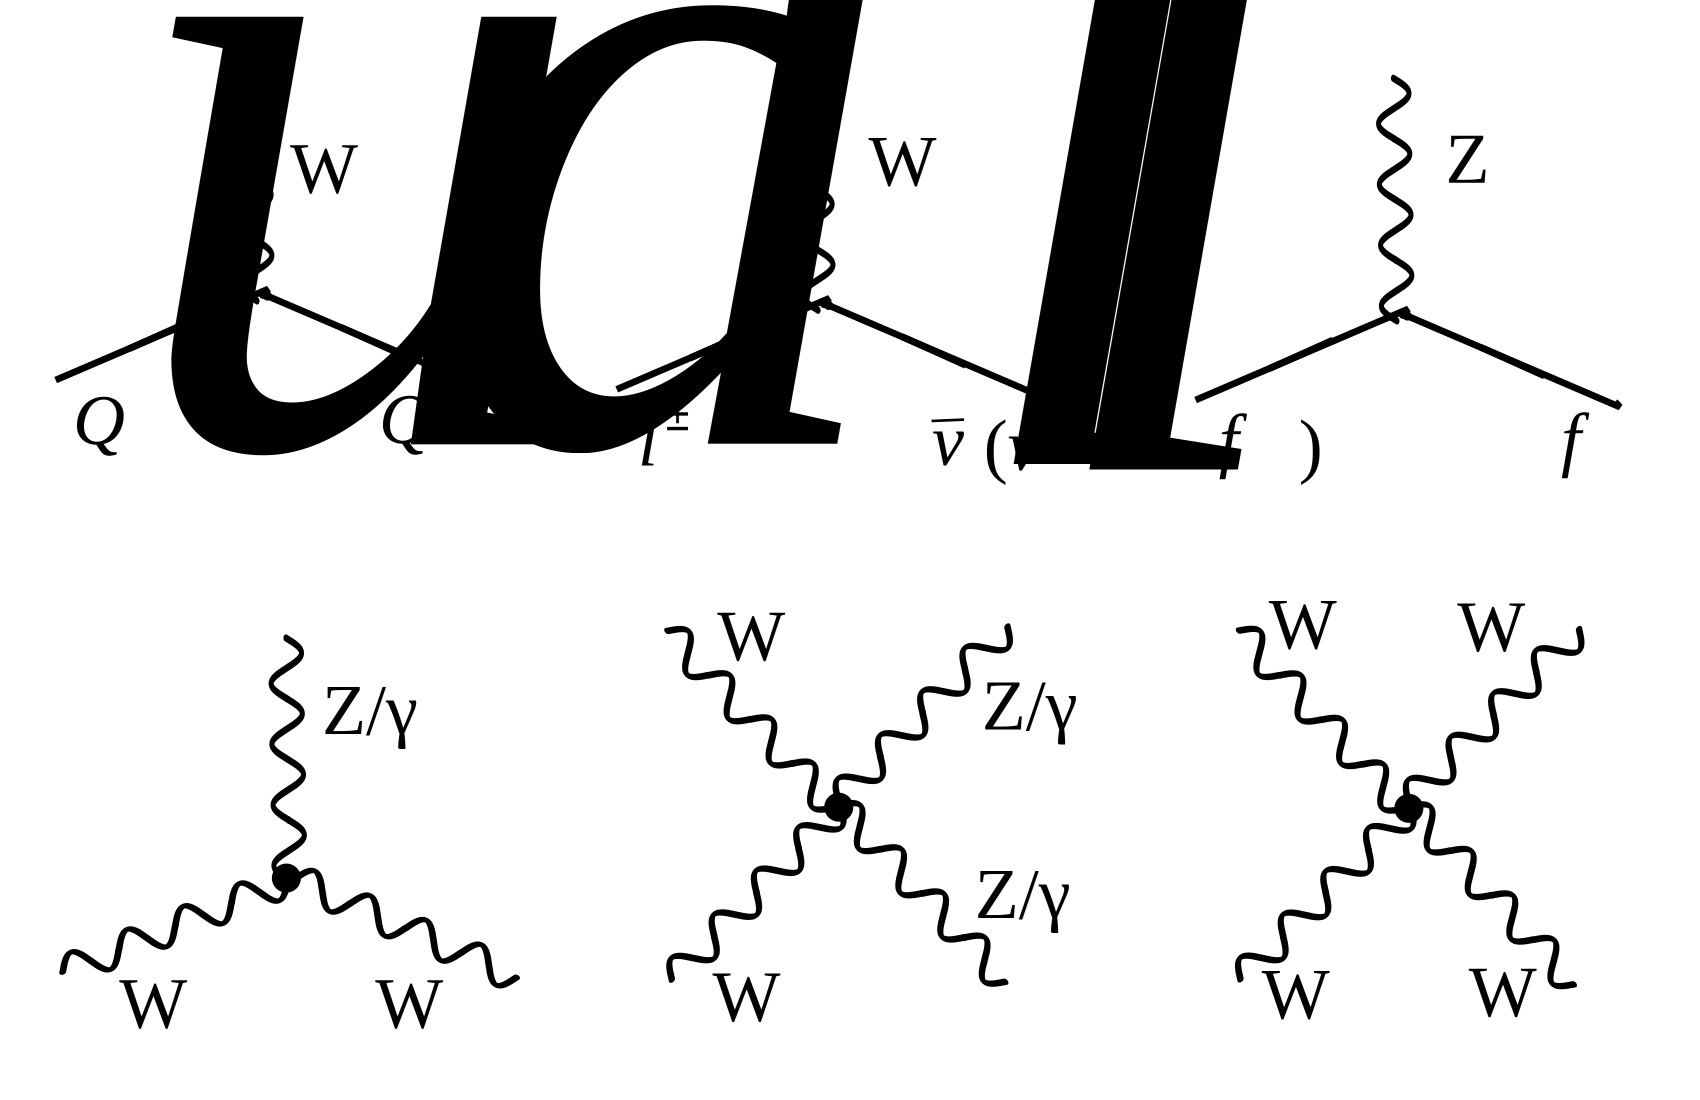
\includegraphics[width=0.90\textwidth]{../figs/Intro/feynmW.png}}
    \caption{Weak interations}
    \label{fig:feynmW}
  \end{center}
\end{figure}


As for the weak interactions, there are two kinds of them: neutral (mediated by a Z boson) and charged (mediated by a W$\pm$ boson). Elementary processes with W and Z bosons are shown in Fig. \ref{fig:feynmW}. Because the electric charge must be conserved at any vertex, a particle radiating or absorbing a W boson converts to a different particle. Thus, a charged lepton converts to a neutrino (or vice versa) as shown in Fig. \ref{fig:feynmW}, top left. A lepton flavor number is always conserved in such interactions (lepton flavor numbers assigned to different lepton are summarized in Tab. \ref{tab:LeptonFlavorNumber}), thus an electron always converts to an electron neutrino, a muon always converts to a muon neutrino etc.\\

 \begin{table}[h]
  \begin{center}
  \caption{ Lepton Flavor Number}
  \begin{tabular}{|c|c|c|c|}
     particles & $L_e$ & $L_{\mu}$ & $L_{\tau}$ \\ \hline
     $e^-,\nu_e$ &  +1  &  0  &  0  \\ \hline 
     $e^+, \bar{\nu_e}$ &  -1  &  0  &  0  \\ \hline 
     $\mu^-,\nu_{\mu}$ &  0  &  +1  &  0  \\ \hline 
     $\mu^+, \bar{\nu_{\mu}}$ &  0  &  -1  &  0  \\ \hline 
     $\tau^-,\nu_{\tau}$ &  0  &  0  &  +1  \\ \hline 
     $\tau^+, \bar{\nu_{\tau}}$ &  0  &  0  &  -1  \\ \hline 
  \end{tabular}
  \label{tab:LeptonFlavorNumber}
  \end{center}
 \end{table}

From top middle diagram in Fig. \ref{fig:feynmW} we see that if a quark with Q=-1/3 enters, then a quark with Q=+2/3 escapes and, therefore, the flavor of the quark has changed. The charged weak interaction is the only interaction which changes a quark flavor. The probability of each of three quarks with Q=+2/3 to be born is determined by the Cabibbo–Kobayashi–Maskawa matrix and is the highest for the quark of the same generation as an initial state quark (in this particular case, $d$ is the initial state quark and $u$ has the highest probability to be produced after an interaction with a W boson but $c$ and $t$ can also be produced if there is enough energy).\\

An elementary process of a neutral weak interactions is an emission of a Z boson off a fermion line (right top diagram in Fig. \ref{fig:feynmW}). An electron is shown here as an example however it also could be any lepton, antilepton, quark or antiquark. Diagrams with a Z boson are very similar to ones with a photon except a photon can only be radiated off a charged particle but a Z boson can also be radiated off a neutrino or antineutrino.\\

The bottom diagrams in Fig. \ref{fig:feynmW} are gauge coupling diagrams. Gauge couplings include self-coupling of a W boson, its interaction with Z boson and its electromagnetic radiation of a photon. WWZ, WW$\gamma$, WWZZ, WWZ$\gamma$, WW$\gamma\gamma$ and WWWW vertices are all possible in the SM.\\

Electromagnetic and weak interactions are unified by the electroweak theory. This theory considers these two forces as different manifestations of the electroweak force. While both forces can be described by very similar formalism, there is also a big difference between them: weak interactions are mediated by heavy bosons ($M_W=80$ GeV, $M_Z=91$ GeV) while electromagnetic interactions are described by a massless photon. \\

To explain this phenomenon, the Higgs mechanism was introduced. The mechanism predicted an existence of an additional boson - the Higgs boson. The Higgs boson was a missing piece of the SM for many years and was finally discovered in 2012 at the LHC by ATLAS and CMS collaborations through the processes shown in Fig.\ref{fig:higgsProduction}.\\ 

\begin{figure}[htb]
  \begin{center}
    {\includegraphics[width=0.95\textwidth]{../figs/Intro/FeynmanHiggs.png}}
    \caption{Higgs production and decay}
    \label{fig:higgsProduction}
  \end{center}
\end{figure}

The measurement in this dissertation is an electroweak measurement because the process involves a W boson. It includes an interaction of a W boson with leptons and quarks as well as the gauge coupling WW$\gamma$. Thus, the measurement is a good test of the SM electroweak theory.\\ 




\subsection{Strong Interactions}
\label{sec:Intro_QCD}

\begin{figure}[htb]
  \begin{center}
    {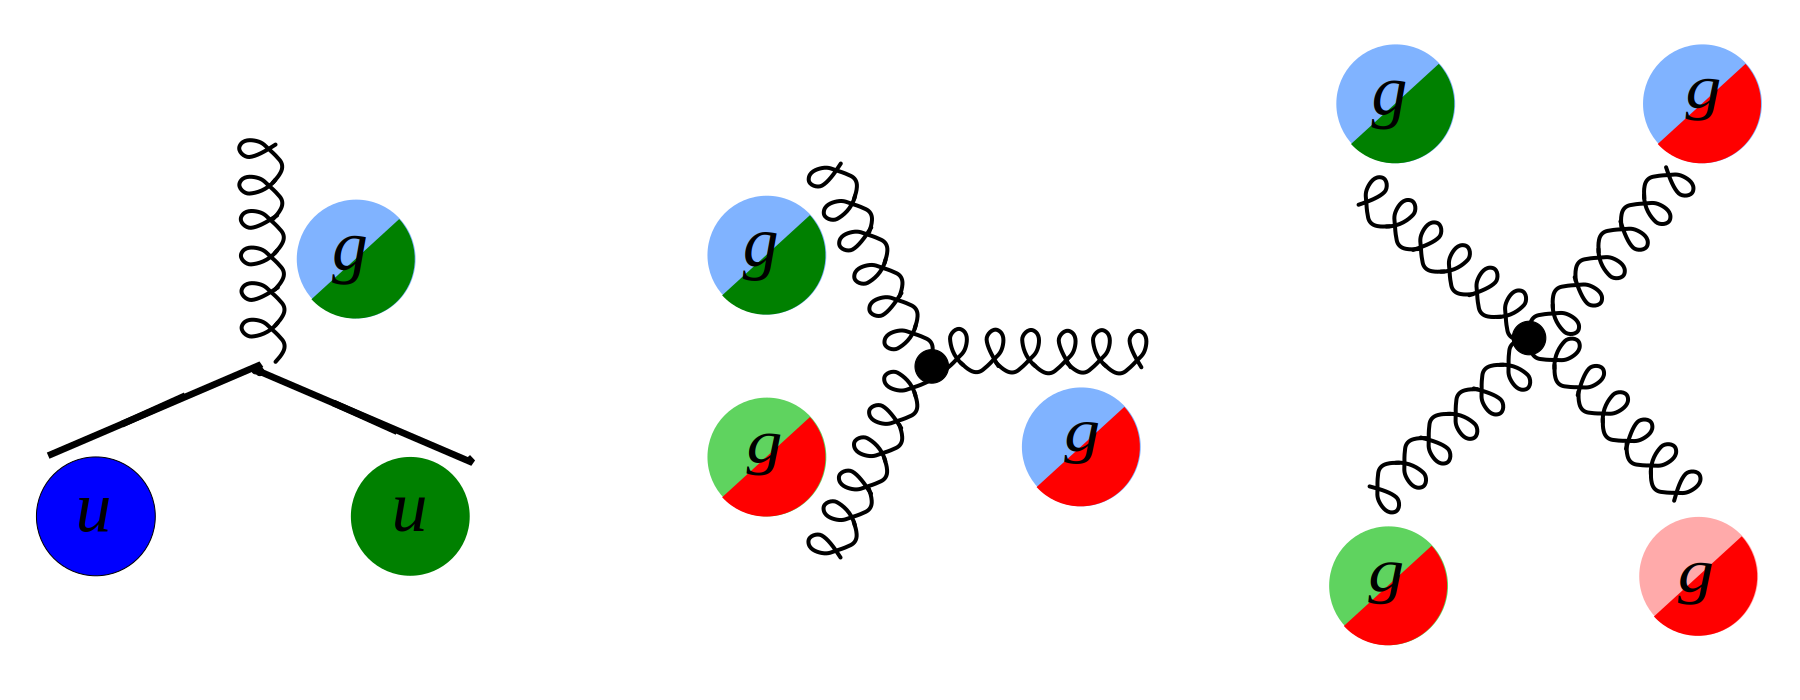
\includegraphics[width=0.90\textwidth]{../figs/Intro/feynmStrong.png}}
    \caption{Strong interations}
    \label{fig:feynmStrong}
  \end{center}
\end{figure}

 %  Again, I do not see a connective narrative. Paragraphs are sets of loosely connected sentences, the section is a set of loosely connected paragraphs. Needs imporvement.
% Somewhat reverse flow of ideas, example:
% > There are eight types of gluons corresponding to different color-anticolor combinations.
% > Gluons are spin-one massless electrically neutral particles.
% First, you should say what gluons ARE, and then you can say what types of gluons exist.
% > Gluons possess color charges, therefore, they can self-interact.
% The emphasis of this statement is that gluons possess color charges, which is odd because you already mentioned it some number of times above (which adds to the feeling of reverse flow).
% Instead, the emphasis of the sentence should be that they can self-inteact.
% Some incorrect information, for example:
% "it becomes larger as the distance becomes smaller” about the coupling constant: it becomes smaller at smaller distances, larger at larger distances.

The third fundamental force after the electromagnetic and weak ones is the strong force. The strong force is responsible for glueing protons and neutrons together in the nuclea as well as for forming protons and neutrons themselves. The strong interactions are performed by exchanging gluons which are spin-one massless electrically neutral particles.  \\

The elementary strong processes are shown in Fig. \ref{fig:feynmStrong}. There are three elementary processes: qqg, ggg and gggg, all are involving particles with color charges. Thus, gluons couple to quarks and self-couple. Color charges must be conserved at each elementary process of the strong interaction. And because quarks can possess three colors, there are eight types of gluons to cover all possible color exchanges. \\

The coupling constant of the strong interaction depends on a distance between interacting particles: it becomes larger as the distance becomes larger. This property leads to two consequences specific to the strong force: the confinement and the asymptotic freedom.\\

The confinement is the property of quarks to always stay in the colorly neutral combinations (hadrons), it forbids the existence of free quarks. A combination becomes colorly neutral when there is the same amount of color and anticolor or if there is the same amount of each of the three colors.  There are two types of hadros: mesons (comprised of a quark and antiquarks with the opposite color charges) and baryons (comprised of three quarks: a red, a green and a blue one). The widely known particles a proton and a neutron are baryons.\\

The asymptotic freedom means that when quarks are very close to each other they almost do not interact with each other and therefore they are free. When the distance between quarks is low which corresponds to high energy, and thus the coupling constant $1/\alpha_s \ll 1$ is low, the strong interactions can be described by a perturbative quantum field theory which is called quantum chromodynamics (QCD).\\

The W$\gamma$ process being measured in this dissertation is not intended to test QCD, but a good understanding of QCD is essential for performing this measurement. First of all, QCD describes the dynamics of quarks and gluons within colliding protons and predicts probabilities of one or another quark-antiquark pair to annihilate. Secondly, the QCD corrections to the Feynman diagrams of the process are large and has to be taken into account in producing simulation. Possible QCD correction include quark-gluon loops at any of three quark lines as well as exchanges of gluons between different quark lines.\\
 

\subsection{Physcis of Proton-Proton Collisions}
Physcis of Proton-Proton Collisions

\section{Open Questions of the Standard Model}


While the SM is an accurate description of all particle physics experimental results, there are certain phenomena which are not included into the SM. In this subsection we discuss some of them.

The gravitational interactions do not fit into the SM. It is the open question whether the quantum theory of gravity is possible and whether there is a mediator of the gravitational interactions. Also, it is not known why the gravitational force is so much weaker than the other forces. One possible explanation comes from a theory which predicts extra spatial dimensions beyond the three we experience (e.g. the string theory). In this case, it is possible that the gravitational force is shared with other dimensions and only a fraction is available in our three dimensions.

Another mystery of the universe is its composition: it is known from the studies of the gravitational effects that our universe consists of dark energy by 68\%, of dark matter by 27\% and of baryon matter only by 5\%~\cite{ref_NASA}. The dark energy resists the gravitational attraction and accelerates the expansion of the universe, and is not detectable by any effects except gravitational. The understanding of dark energy is a question of general relativity rather than particle physics. The dark matter, however, likely consists of particles and therefore is a subject of particle physics. It does not radiate and that is why it cannot be detected by telescopes. The nature of the dark matter is not known but its constituents must be very stable to remain since the Big Bang. The theory of the supersymmetry which is unifying fundamental particles and mediators predicts many of new heavy particles and the lightest supersymmetric particle, the neutralino, is a good candidate for dark matter.

One more open question is the reason for the matter/antimatter asymmetry. Matter and antimatter should have been created in the same amount at the moment of the Big Bang. Most of it has annihilated but because of asymmetry, there was more matter than antimatter which led to the state of the Universe we observe now. There is a phenomenon of the CP-violation in weak interactions observed and described which predicts the asymmetry at a certain level. However, the effect of the CP-violation is not large enough to account for the observed amount of the matter and, therefore, the total matter/antimatter asymmetry remains unexplained. 

The measurement of the $W\gamma$ production in $pp$ collisions has a goal to both test the SM and search for the BSM physics. We measure a cross section differential in the component of the photon momentum, transverse to the beamline (referred as photon transverse momentum, or $P_T^{\gamma}$). The low $P_T^{\gamma}$ region is not expected to be affected by any new physics and must agree well with the SM predictions while the high $P_T^{\gamma}$ region may indicate an existence of new physics if there is an enhancement over the SM predictions. The excess would be indirect evidence of the BSM particles like supersymmetric particles or additional gauge bosons which could be part of the explanation of the dark matter presence or difference in magnitudes of different interactions. More theoretical details about the SM description of W$\gamma$ process as well as possible BSM physics are given in Ch.~\ref{sec:WgAbout}.    

%Grand unification and super unification



\section{W$\gamma$ Production Theory and Former Experimental Results} % 5-10 pages
\label{sec:WgAbout}

Chapter~\ref{sec:WgAbout} provides deeper theoretical background for the measurement of this dissertation and discusses former experimental results. The derivation of the electroweak Lagrangian is described in Ch.~\ref{sec:WgAbout_SMEWK}, including the appearance of TGC and QGC terms. Then concepts of the cross section and the luminosity are discussed in Ch.~\ref{sec:WgAbout_LumiAndCS}. More specific details regarding the SM cross section of W$\gamma$ are summarized in Ch.~\ref{sec:WgAbout_SMproduction}. Possible causes and potential effects of aTGC are explained in Ch.~\ref{sec:WgAbout_ATGC}. Finally, Ch.~\ref{sec:WgAbout_PastMeasurements} lists former physics experiments which probed the same aTGC vertex which is probed in the measurement of this dissertation including measurments of exactly the same process at lower LHC beam energy.\\


\subsection{Electroweak Theory of the Standard Model}
\label{sec:WgAbout_SMEWK}

%Pich, 1

The SM is a gauge theory invariant under the local $SU(3)_C x SU(2)_L x U(1)_Y$ transformation. $SU(3)_C$ stands for color transformations and, therefore, the $SU(3)_C$-invariant Lagrangian describes QCD. It is designed to describe color interactions of quarks and antiquarks. The requirement to satisfy the gauge invariance generates eight massless gluons. The non-abelian nature of the $SU(3)$ group leads to self-interactions of gluons, particularly to the appearance of three-gluon and four-gluon vertices.\\

The Lagrangian based on the $SU(2)_L x U(1)_Y$ symmetry describes unified theory of electroweak interactions. The requirement of the local gauge invariant generates four massless vector bosons which are mediators of electromagnetic and weak interactions. The non-abelian structure of $SU(2)$ group introduces gauge boson couplings just like self-interactions of gluons appear in QCD. However, it is experimentally known that mediators of weak interactions are heavy particles with masses $M_W=80$~GeV and $M_Z=91$~GeV. To introduce these masses, the electroweak symmetry has to be spontaneously broken to the QED symmetry group $U(1)$:\\

$SU(2)_L \times U(1)_Y \rightarrow U(1)_{QED}$\\

The Spontaneous Symmetry Breaking (SSB) introduces an additional particle into the SM: the Higgs boson ($H$) and generates masses for $W$ and $Z$ bosons. A photon is a massless particle, therefore, $U(1)_{QED}$ symmetry remains unbroken and a photon does not couple to a Higgs boson.\\

The Lagrangian transformations of the SM are described in \cite{ref_Pich} for QED, QCD, unified electroweak force and the Higgs mechanis. The measurement in this dissertation provides a test for the electroweak sector of the SM, thus we will repeat here the theoretical path from the Lagrangians of free particles to the accomodation of the electroweak gauge bosons including their self-couplings.\\

%Pich, 3.1
% introduce hirality/helicity
There are certain features of weak interactions whach are known experimentally and they all have to be accomodated by the theory. It is known that only left-handed fermions and only right-handed antifermions couple to a $W$ boson.\\ 

A $Z$ boson couples to both left-handed and right-handed fermions and antifermions but with different strength while photon-fermion couplings do not depend on chirality but on electric charge only. As for the neutrinos, only left-handed neutrinos and right-handed antineutrinos found to couple to a $Z$ boson, therefore, right-handed neutrinos and left-handed antineutrinos were not found to participate in any SM interactions.\\

Given different properties of left-handed and right-handed particles, they are treated differently by the electroweak theory. $SU(2)$ doublets are introduced for the wave functions of left-handed particles while $SU(2)$ singlets are introduced for the wave functions of right-handed particles.\\ 
 
%Pich 3.2

\begin{equation}\label{eq:psi_for_quarks}
\psi_1(x)=\begin{pmatrix} u \\ d \end{pmatrix}_L \text{, } \psi_2(x)=u_R \text{, } \psi_3(x)=d_R \text{.}
\end{equation}

\begin{equation}\label{eq:psi_for_leptons}
\psi_1(x)=\begin{pmatrix} \nu_e \\ e^- \end{pmatrix}_L \text{, } \psi_2(x)=\nu_{eR} \text{, } \psi_3(x)=e^-_R \text{. }
\end{equation}

Consider the free Lagrangian:\\

\begin{equation}\label{eq:L_free}
L_0 = \sum_{j=1}^{3} i \bar{\psi_j}(x) \gamma^\mu \partial_\mu \psi_j(x) 
\end{equation}

where $\gamma^\mu$ are Dirac matrices \cite{ref_Griffiths}.\\

The wave function $\psi_1$ changes under the $SU(2)_L \times U(1)_Y$ transformations in the following way:\\

\begin{equation}
\psi_1(x) \rightarrow e^{i y_1 \beta} U_L \psi_1(x)
\end{equation}


The wave functions $\psi_{(2,3)}(x)$ are singlets of $SU(2)_L$ and are affected only by $U(1)$ transformations:\\

\begin{equation}
\psi_{(2,3)}(x) \rightarrow e^{i y_{(2,3)} \beta} \psi_{(2,3)}(x)
\end{equation}

The transformation $U_L \equiv e^{i \sigma_i \alpha_i /2}$, $\sigma_i$ are Pauli matrices \cite{ref_Griffiths}, $\alpha_i(x)$ and $\beta(x)$ are arbitrary functions, $y_{(1,2,3)}$ are hypercharges.\\

In order to satisfy the local Largangian invariance, partial derivatives in \ref{eq:L_free} has to be substituted with covariant derivatives:\\

\begin{equation}\label{eq:L_free_covariant}
L_0 \rightarrow L = \sum_{j=1}^{3} i \bar{\psi_j}(x) \gamma^\mu D_\mu \psi_j(x) 
\end{equation}

where\\

\begin{equation}
D_\mu \psi_1(x) = [\partial_\mu - i g {\tilde{W}}_\mu(x) - i g' y_1 B_\mu(x) ] \psi_1(x) 
\end{equation}

\begin{equation}
D_\mu \psi_{(2,3)}(x) = [\partial_\mu - i g' y_{(2,3)} B_\mu(x) ] \psi_{(2,3)}(x) 
\end{equation}

where ${\tilde{W}}_\mu(x) \equiv \frac{\sigma_i}{2} W_\mu^i(x) = \frac{1}{\sqrt{2}} 
\begin{pmatrix}
\sqrt{2} W_\mu^3 & (W_\mu^1 - i W_\mu^2)/{\sqrt{2}}\\
(W_\mu^1 + i W_\mu^2)/{\sqrt{2}} & -W_\mu^3\\
\end{pmatrix}$.

The Lagrangian $L$ from Eq.~\ref{eq:L_free_covariant} is now invariant under local $SU(2)_L \times U(1)$ transformations. Four vector boson fields appear in $L$: $B_\mu$, $W_\mu^1$, $W_\mu^2$, $W_\mu^3$.  Thus, it is necessary to add terms for kinetic energies of the vector bosons:\\

\begin{equation} \label{eq:L_gauge_kin}
L_{KIN}=-\frac{1}{4}B_{\mu\nu}B^{\mu\nu}-\frac{1}{4}W_{\mu\nu}^i W^{\mu\nu}_i
\end{equation}

where $B_{\mu\nu} \equiv \partial_\mu B_\nu - \partial_\nu B_\mu$, $W_{\mu\nu}^i \equiv \partial_\mu W_\nu^i - \partial_\nu W_\mu^i + g \epsilon^{ijk} W_\mu^j W_\nu^k$\\

Off-diagonal terms of ${\tilde{W}}_\mu$ are wave functions of charged vector bosons $W^{\pm}=W_\mu^1 \mp i W_\mu^2)/{\sqrt{2}}$ while $W_\mu^3$ and $B_\mu$ are neutral fields corresponding to a $Z$ boson and a photon. However, $W_\mu^3$ couples to left-handed fermions only while a $Z$ boson is known to interact with particles with both helicities.\\

Then the neutral electroweak mixing is introduced:\\

\begin{equation}
  \begin{pmatrix} W_\mu^3 \\ B_\mu \end{pmatrix} \equiv
  \begin{pmatrix} \cos \theta_W & \sin \theta_W \\ -\sin \theta_W & \cos \theta_W \end{pmatrix}
  \begin{pmatrix} Z_\mu \\ A_\mu \end{pmatrix}
\end{equation} 

where $\theta_W$ is an electroweak mixing angle, $A_\mu$ is a photon field.\\

Terms involving $A_\mu$ in the electroweak Largangian must be equal to the corresponding terms in QED Lagrangian:\\

\begin{equation}\label{eq:L_QED}
L_{QED} = i \bar{\psi}(x) \gamma^\mu \partial_\mu \psi(x) - m \bar{\psi}(x) \psi(x) + e Q A_\mu(x) \bar{\psi}(x) \gamma^\mu \psi(x) - \frac{1}{4} A_\mu\nu(x) A^{\mu\nu}(x)
\end{equation}

This requirement relates $g$, $g'$, $\theta_W$ and $e$ as\\

$g \sin \theta_W = g' \cos \theta_W = e$\\

and provides expression for weak hypercharges:\\

$Y = Q - T_3$,\\

where $T_3 = \sigma_3 / 2$, $Q_1 = \begin{pmatrix} Q_{u/\nu} & 0 \\ 0 & Q_{d/e} \end{pmatrix}$, $Q_2 = Q_{u/\nu}$, $Q_3=Q_{d/e}$.\\

If substitute $W_\mu^i$ and $B_\mu$ in $L$ from Eq. \ref{L_gauge_kin} with the wave functions of $W^\pm$, $Z$ and a photon, charged TGC and QGC terms will apeear as shown in Eq.~\ref{eq:L_TGC_1} and Eq.~\ref{eq:L_QGC_1} but not neutral TGC or QGC vertex would be generated.\\

\begin{equation} \label{eq:EWK_Zg_bosons_mixing}
B_\mu = -sin \theta_W Z_\mu + cos \theta_W A_\mu \text{, } W_\mu^3 = cos \theta_W Z_\mu + sin \theta_W A_\mu
\end{equation}
\begin{equation} \label{eq:EWK_Zg_bosons_mixing}
W_\mu^1 = \sqrt{2}(W^+ + W^-) \text{, }W_\mu^2 = \sqrt{2}(W^- + W^+)
\end{equation}

\begin{equation} \label{eq:L_TGC_1}
L_{TGC} = -\frac{g}{4}(\partial_\mu W_\nu^i - \partial_\nu W_\mu^i)\epsilon^{ijk}W^{\mu j}W^{\nu k} - \frac{g}{4}\epsilon^{ijk}W_\mu^j W_\nu^k (\partial^\mu W^{\nu i} - \partial^\nu W^{\mu i})
\end{equation}

\begin{equation} \label{eq:L_QGC_1}
L_{QGC} = -\frac{g^2}{4} \epsilon^{ijk} \epsilon^{ilm} W_\mu^j W_\nu^k W^{\mu l} W^{\nu m}
\end{equation}

\begin{equation} \label{eq:L_TGC_2}
L_{TGC} = L_{TGC}^{(1)} + L_{TGC}^{(2)}
\end{equation}

\begin{equation} \label{eq:L_TGC_2_1}
L_{TGC}^{(1)} = -ie \cot \theta_W (W^{-\mu\nu} W^{+}_\mu Z_\nu - W^{+\mu\nu} W^-_\mu Z_\nu +W^-_\mu W^+_\nu Z^{\mu\nu}) 
\end{equation}

\begin{equation} \label{eq:L_TGC_2_2}
L_{TGC}^{(2)} = - ie(W^{-\mu\nu}W^+_\mu A_\nu - W^{+\mu\nu}W^-_\mu A_\nu + W^-_\mu W^+_\nu A^{\mu\nu})
\end{equation}

\begin{equation} \label{eq:L_QGC_2}
L_{QGC} = L_{QGC}^{(1)} + L_{QGC}^{(2)} + L_{QGC}^{(3)} + L_{QGC}^{(4)}
\end{equation}

\begin{equation} \label{eq:L_QGC_2_1}
L_{QGC}^{(1)} = -\frac{e^2}{2\sin^2 \theta_W}(W^+_\mu W^{-\mu}W^+_\nu W^{-\nu} - W^+_\mu W^{\mu +} W^-_\nu W^{-\nu})
\end{equation}

\begin{equation} \label{eq:L_QGC_2_2}
L_{QGC}^{(2)} = - e^2 \cot^2 \theta_W (W^+_\mu W^{-\mu} Z_\nu Z^{\nu} - W^+_\mu Z^{\mu} W^-_\nu Z^{\nu})
\end{equation}

\begin{equation} \label{eq:L_QGC_2_3}
L_{QGC}^{(3)} = - e^2 \cot \theta_W (2 W_\mu^+ W^{-\mu} Z_\nu A^{\nu} - W^{+}_\mu Z^\mu W^-_\nu A^\nu - W^{+}_\mu A^\mu W^-_\nu Z^\nu)
\end{equation}

\begin{equation} \label{eq:L_QGC_2_4}
L_{QGC}^{(4)} = - e^2 (W^+_\mu W^{-\mu} A_\nu A^{\nu} - W^+_\mu A^{\mu} W^-_\nu A^{\nu})
\end{equation}

Because left-handed and right-handed wave functions transform differently under the electroweak symmetry, fermion mass terms would not be invariant and, therefore, are forbidden. Mass terms for gauge bosons also would violate the Lagrangian invariance. Therefore, Largangian $L$ in Eq. \ref{eq:L_free_covariant} contains massless particles only.\\

To introduce masses into the electroweak Lagrangian, an $SU(2)_L$ doublet of complex scalar fields $\phi(x)$ is added to the Lagrangian (Eq.~\ref{eq:H_doublet}).\\

\begin{equation}\label{eq:H_doublet}
  \phi(x) \equiv \begin{pmatrix} \phi^{(+)}(x) \\ \phi^{(0)}(x) \end{pmatrix}
\end{equation}

One of the components of the doublet involves a new particles, the Higgs boson \cite{ref_Pich}. Masses of $W$ and $Z$ bosons and charged fermions aquire their masses through couplings to the Higgs boson. The strength of the coupling constant is proportional to the square of the particle's mass, therefore, massless particles do not couple to $H$.\\

The mechanism of generating a fermion's mass involve both left-handed and right-handed components of the fermion. If our hypothesis that right-handed neutrinos do not exist, then the Higgs mechanism does not generate neutrino masses. However, from the experiments of neutrino oscillations, neutrinos are known to have masses even though their masses are much smaller than masses of other fermions. Several hypotheses were offered to resolve this contradiction however at the moment the mechanism of neutrinos to acquire masses remain unknown \cite{ref_PDG}.\\


\subsection{Cross Section and Luminosity}
\label{sec:LumiAndCS}

In this dissertation we are measuring the total cross section of the process $pp \rightarrow l \nu_l \gamma + X$ and its differential cross section in transverse momentum of the photon. The cross section in particle physics is the interaction probability per unit flux of incident particles~\cite{ref_fnal_LumiCS}. It can be interpreted as area which must be crossed by an incident particle in order to interact with a scattering center, or, in case of a differential cross section, area $d\sigma$ within which an incident particle must appear to be scattered off by an angle $d\theta$ (Fig.~\ref{fig:CSclassical}). The relationship between $d\sigma$ and $d\theta$ gives us the expression for a differential cross section $d\sigma/d\theta$. Integrating over $d\theta$, one would get the total cross section $\sigma$. \\

In Fig.~\ref{fig:CSclassical} an incident particle is the same as a final state particle, however in particle physics final state particles can differ from initial state particles, and we measure a differential cross section with respect to a parameter $X$ of the final state particle. Differentiating $\sigma$ by $X$ we get the expression for the differential cross section $d\sigma/dX$.\\

\begin{figure}[htb]
  \begin{center}
    {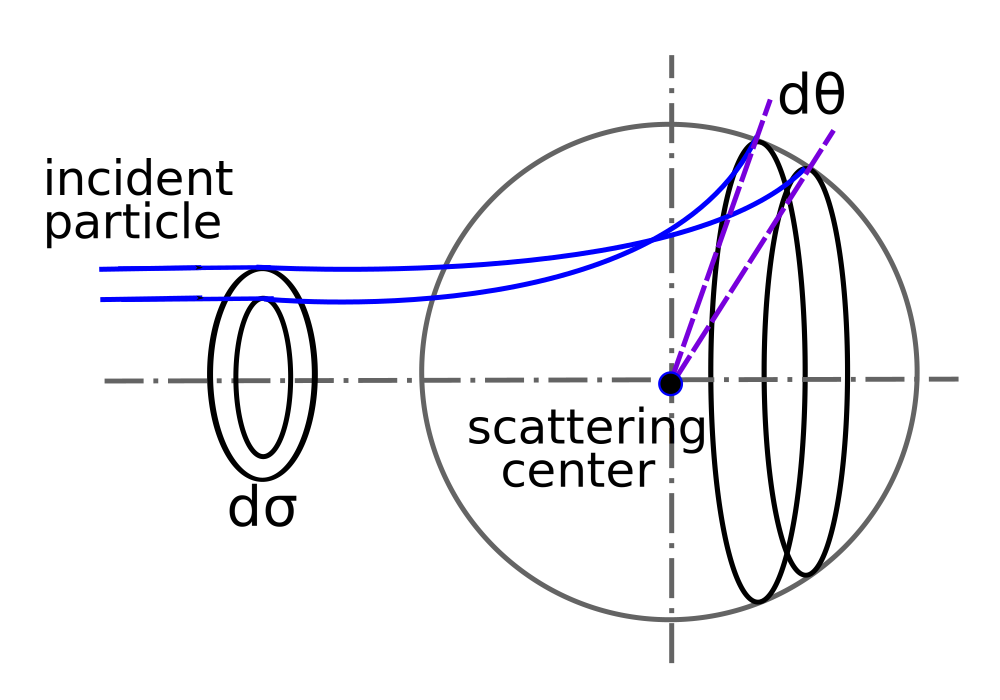
\includegraphics[width=0.70\textwidth]{../figs/WgAbout/CSclassical.png}}
    \caption{Illustration of the differential cross section concept in the classical case.}
    \label{fig:CSclassical}
  \end{center}
\end{figure}

Referring to the Fig.~\ref{fig:CSclassical}, a number of particles passing through the area $\sigma$ per unit time is $N=L \cdot \sigma$, where $L$ is the flux of incident particles and is called luminosity. Therefore, the cross section $\sigma$ of a specific process can be determined from an experiment as $\sigma=N/L$. \\

A cross section also can be computed theoretically. The formula to compute a cross section is:\\

\begin{equation}
  \sigma = \frac{W_{fi}}{L} N_{fs},
\end{equation}

where $W_{fi}$ is a transition probability between final and initial states of the system per unit volume, $L$ is the flux of initial particles, and $N_{fs}$ is the density of final states~\cite{ref_Halzen_Martin},~chapter~4.3.\\ 

The formula of the cross section is called the Fermi's Golden Rule~\cite{ref_Griffiths}. In case of the scattering of two particles to three final state particles $1+2\rightarrow 3+4+5$, it takes the following form:\\
%Further on, you do mention amplitude several times, but you never explain what it is. You may want to discuss probability amplitudes, connecting initial and final states, etc, with some basic quantum mechanics bra-ket notations, etc.
%You do not need to derive it. But you need to explain, I think, how it comes about and what it means. Just a few more sentences would be enough.

\begin{equation}\label{eq:FermiGoldenRule}
  \sigma = \frac{ 1 }{4\sqrt{(p_1p_2)^2-(m_1m_2)^2}} \int |M|^2 (2\pi)^4 \delta^4(p_1+p_2-p_3-p_4-p_5) \prod_{j=3}^{5} \frac{1}{2 \sqrt{\bar{p_j^2}+m_j^2 }}\frac{d^3\bar{p_j}}{(2\pi)^3},  
\end{equation}

where $p_i$ are 4-momenta and ${\bar{p_i}}$ are three momenta of the initial state and the final state particles, $m_i$ are masses of particles, $M$ is the process amplitude determined by the dynamics of the particles interaction. All available momenta of the final state particles is called the phase space.\\ 
%Consider discussing parton luminosity and the cross section expression that involves the PDFs and parton-based cross sections

The cross section of the hard scattering in proton-proton collisions $pp \rightarrow X+Y$ has two ingridients: PDFs and a partonic cross section $\sigma_{ab\rightarrow X}$. The partonic cross section is described by perturbative QCD while PDFs require non-perturbative computations and are determined, in part, from experiments (Fig.~\ref{fig:pdfs}). According to the QCD factorization theorem~\cite{ref_HardScattering}:\\
%The paragraph on the lines 473 - 478. I think you need to explain a bit more. Why can we factorize into partonic cross sections? I suggest you refer to the discussion of the proton structure in section 1.4, to the partons and parton PDFs discussed there. You also need to explain what are “i”, “j”, what are x1, x2, etc.

\begin{equation}\label{eq:ppCS_general}
  \sigma(pp \rightarrow X+Y)= \sum_{a,b} \int dx_a dx_b f_a(x_a,Q^2) f_b(x_b, Q^2) \sigma(ab \rightarrow X).
\end{equation}
%Another question I forgot to mention: in the equation 28 you have Q2. There is no integration over Q2. So what happens to it? Is it that the cross section defined by this equation a function of Q2?

In case of $W\gamma$ process, $X$ is $l \nu \gamma$, $ab$ are $q_i \bar{q}_j$ or $q_j \bar{q}_i$. $Q^2$ is the large momentum scale that characterizes hard scattering, $f_a$ and $f_b$ are PDFs, $x_a$ and $x_b$ are fractions of momenta of the partons.\\

\section{Standard Model $W\gamma$ Production}
\label{sec:WgAbout_SMproduction}

A $W$ boson in proton-proton collisions can be produced in the processes $q {\bar{q'}} \rightarrow W$ where $q$ and $\bar{q'}$ are a quark and an antiquark which have a total charge of $+1$ if producing a $W^+$ boson or $-1$ if producing a $W^-$ boson. The processes $u\bar{d}\rightarrow W^+$ and $d\bar{u}\rightarrow W^-$ are the most likely to occur because $u$ and $d$ are valence quarks in a proton. There are twice as many $u$ quarks in a proton as $d$ quarks, therefore, $W^+$ is produced twice more frequently than $W^-$. Antiquarks $\bar{d}$ and $\bar{u}$ come from the sea $q\bar{q}$ pairs of the other proton.

Once created, a $W$ boson decays immediatelyi, its lifetime is~$\simeq 10^{-25}$~s. In an experiment one detects its decay products rather than the $W$ boson itself. Decay modes of a $W$ boson include $W^\pm \rightarrow l^\pm \nu_l ({\bar{\nu_l}})$ where $l^\pm=e^\pm$, $\mu^\pm$ or $\tau^\pm$ with branching fractions of ~11\% per a leptonic channel \cite{ref_PDG}. The remaining 67\% account for various $W\rightarrow q\bar{q'}$ decays. In this dissertation we only consider $W^\pm \rightarrow \mu^\pm \nu_\mu ({\bar{\nu_\mu}})$ and $W^\pm \rightarrow e^\pm \nu_e ({\bar{\nu_e}})$ channels.

% MAY NOT NEED THIS
%Mass of a $W$ boson $M_W=80$ GeV is much larger than masses of its decay products: $M_\mu=105$ MeV, $M_e=0.5$ MeV, $M_\nu<2$ eV. Therefore, almost all mass of a $W$ boson converts to the kinetic energy of the muon or electron and neutrino or antineutrino.\\

A photon can be emitted from any charged particle of the process: a quark, an antiquark, a charged lepton or a $W$ boson (Fig.~\ref{fig:feynmWg_LO_NLO}, top). A quark and an antiquark are initial state particles and, therefore, if one of them radiates a photon, we refer to the process as initial state radiation (ISR). A muon or an electron is a final state particle and if it radiates a photon, we call such a process final state radiation (FSR). Finally, a $W$ boson is a gauge boson and if it radiates a photon, the process has a vertex with three gauge bosons: $WW\gamma$, and we call such process the triple gauge coupling (TGC). We cannot distinguish between these processes experimentally because we detect final state particles only.

\begin{figure}[htb]
  \begin{center}
    {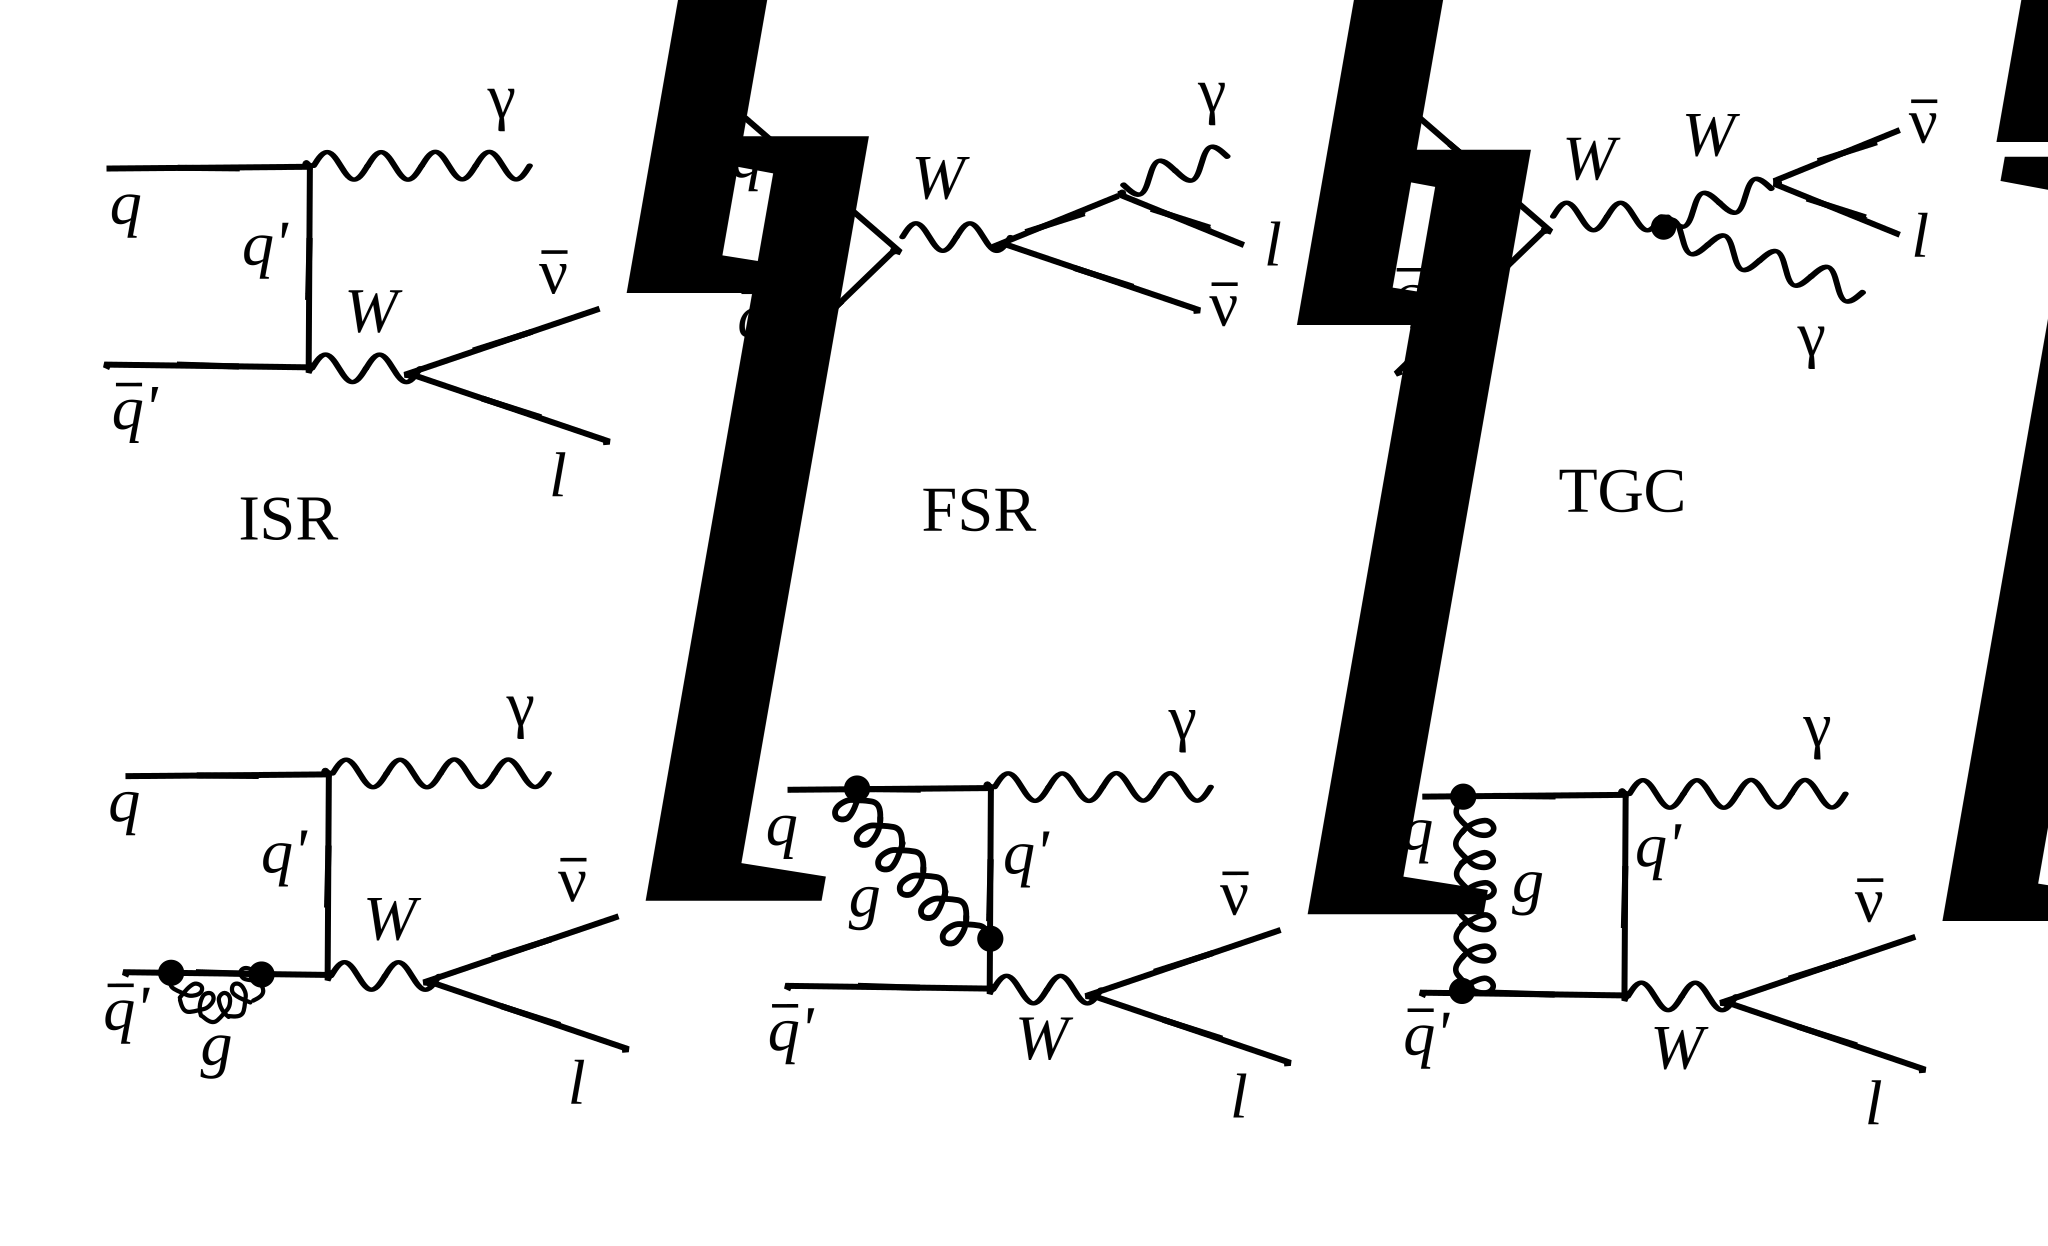
\includegraphics[width=0.90\textwidth]{../figs/WgAbout/feynmWg_LO_NLO.png}}
    \caption{Feynman diagrams of W$\gamma$ production. Top: LO diagrams, bottom: several examples of NLO in QCD.}
    \label{fig:feynmWg_LO_NLO}
  \end{center}
\end{figure}

The electroweak Lagrangian is described in Chapter~\ref{sec:WgAbout_SMEWK}. It is possible to derive equations of motion from the Lagrangian for any fields involved~\cite{ref_Griffiths}. However, in a quantum field theory equations of motion cannot be solved exactly and, therefore, the perturbative approach is used if a coupling constants is $g \ll 1$.

To represent the process graphically Feynman diagrams were invented. Also the diagrams can be used to calculate the process amplitude $M$ in Eq.~\ref{eq:FermiGoldenRule} because they are determined by Lagrangian terms relevant to the process. There are an infinite number of Feynman diagrams corresponding to any specific process and the total amplitude of the process is a sum of individual amplitudes of each diagram and it is not technically possible to take into account all of them. Each vertex introduces a factor in the amplitude of the process that is proportional to the coupling constant. If the coupling constant is $g \ll 1$, the perturbative approach arranges all the diagrams by orders of contribution, and, therefore, the Feynman diagrams with fewer vertices would give a significantly larger contribution to the amplitude. In Fig.~\ref{fig:feynmWg_LO_NLO} examples of the Leading Order (LO) and the Next-to-Leading Order (NLO) Feynman diagrams are shown (top and bottom diagrams respectively).

At LO, the W$\gamma$ process is represented by four Feynman diagrams including one FSR, one TGC and two ISR diagrams. Each LO diagram has three vertices. The first calculation of the W$\gamma$ process with necessary expressions can be found in~\cite{ref_theory_LO}.

The NLO corrections to the amplitude of the $W\gamma$ process that are shown in Fig.~\ref{fig:feynmWg_LO_NLO} are QCD corrections only, which include gluon loops at the same quark line and exchange of a gluon between two different quark lines, however, QED and weak NLO diagrams are also possible. QED corrections involve radiations of extra photons by charged particles, exchange of photons between different charged particles or a photon can be radiated and absorbed by the same charged particle forming a loop. Similarly, weak corrections involve extra virtual $W$ or $Z$ bosons. The QCD corrections are the largest among the discussed correction types because the QCD coupling constant is the largest.

A theoretical cross section in particle physics is compared to a measurement result to test the predictions of the model. Also the theoretical cross section is used for producing simulated data. In a simulation, a large set of $pp$ collisions resulting in a physics process of interest is modeled to create a data set that mimics real data. A typical simulation consists of two parts: the generation of the process and the simulation of particles paths through the detector. The first stage contains a collection of events with final state particles with kinematic quantities distributed according to theoretical predictions for a given process. This stage relies on the theory including the cross section and also all dynamics of the process. The second stage simulates the interaction with media during propagation of particles through the model of the detector as well as the response of detector electronics. In its final form, a simulated dataset has the same format and content of detector signals for each event as real data, and can undergo the same reconstruction and analysis procedure as real data would.

The most precise theoretical $W\gamma$ cross section available is the Next-to-Next-to-Leading Order (NNLO) cross section in QCD~\cite{ref_theory_NNLO}. The effects of the NNLO correction over the NLO correction and over the LO result are shown in Fig.~\ref{fig:Theory_NNLO_and_other} for the transverse mass of the final state particles $m_T^{l \nu \gamma}$ and for the rapidity difference between a charged lepton and a photon $\Delta_{l\gamma}$. The NNLO and NLO theoretical predictions for the photon transverse momentum $p_T^\gamma$ are overlaid with the~7~TeV ATLAS result. The contribution from higher order corrections is estimated to be $\pm$4\%. However, the NNLO theoretical result was published only recently, in 2015, and no NNLO $W\gamma$ simulation is available at this time. The simulation used in this analysis is LO + up to two hadronic jets simulation which was found to give the same predictions as the NLO result.
% [REFERENCE to APPENDIX?].\\

\begin{figure}[htb]
  \begin{center}
    {\includegraphics[width=0.95\textwidth]{../figs/WgAbout/Theory_NNLO_PtGamma.png}}    
    {\includegraphics[width=0.95\textwidth]{../figs/WgAbout/Theory_NNLO_mT_finer.png}}
    {\includegraphics[width=0.50\textwidth]{../figs/WgAbout/Theory_NNLO_rapidity.png}}
    \caption{Theory spectra. Top: NLO and NNLO $p_T^\gamma$ spectra of $W\gamma\rightarrow l\nu\gamma$ at $\sqrt{s}=7$~TeV overlaid with ATLAS data for $N_{jet} \geq 0$ (left) and $N_{jet}=0$ (right). Middle: LO, NLO and NNLO $m_T^{l\nu\gamma}$ spectra of $W\gamma\rightarrow l\nu\gamma$ at $\sqrt{s}=7$~TeV for $P_T^\gamma>15$~GeV (left) and $P_T^\gamma>40$~GeV (right). Bottom: LO, NLO and NNLO $\Delta_{l\gamma}$ spectra of $W\gamma\rightarrow l\nu\gamma$ at $\sqrt{s}=7$~TeV.}
    \label{fig:Theory_NNLO_and_other}
  \end{center}
\end{figure}

Certain BSM theories predict an enhancement of the contribution from the TGC diagram over the SM prediction. The discussion of these BSM effects and how they affect the $W\gamma$ process takes place in Ch.~\ref{sec:WgAbout_ATGC}. 


\subsection{Anomalous $W\gamma$ Production}
\label{sec:WgAbout_ATGC}

Triple and quartic gauge couplings (QGC) are represented by vertices with three and four bosons (Fig. \ref{fig:TGC_and_QGC_vertices}). TGC and QGC can be charged or neutral. There are variety of the SM processes where charged TGC and QGC are possible. Such processes can occur through a Feynman diagram with a vertex involving a $W$ boson and conserving charge. Corresponding vertices are $WW\gamma$, $WWZ$, $WWWW$, $WW\gamma\gamma$, $WWZ\gamma$, and $WWZZ$ (Fig. \ref{fig:TGC_and_QGC_vertices}, 1$^st$, 3$^rd$, and 5$^th$ diagrams). To search for the new physics, all these vertices are described by extended Largangian term than the SM description, involving several constants which have known values in the SM. A significant deviation of one of these constants from the known values would be an indication of a new physics.\\

As for neutral TGC and QGC, they are forbidden in the SM at the tree level but extended Lagrangian contains terms which describes neutral TGC and QGC vertices: $Z\gamma\gamma$, $ZZ\gamma$, $ZZZ$, $Z\gamma\gamma\gamma$, $ZZ\gamma\gamma$, $ZZZ\gamma$, and $ZZZZ$. Similarly to charge TGC and QGC cases, neutral TGC and QGC Largangian terms involve contants which are zero in the SM.\\  

%Maybe, general words about ATGC, where does it come from

%How it would affect the distributions and cross section



In $W\gamma$ measurement we can probe $WW\gamma$ vertex only. The most general Lorentz invariant Lagrangian of this vertex takes the following form \cite{ref_theory_aTGC}:\\

$i L_{eff}^{WW\gamma}= e [ g_1^{\gamma} A^\mu (W_{\mu\nu}^- W^{+\nu} - W_{\mu\nu}^+ W^{-\nu}) + \kappa_\gamma W_{\mu}^+ W_{\nu}^- A^{\mu\nu} + {\frac{\lambda_\gamma}{m^2_W}} A^{\mu\nu} W_\nu^{+\rho} W_{\rho\mu}^- + i g_5^\gamma \epsilon_{\mu\nu\rho\sigma}((\partial^\rho W^{-\mu})W^{+\nu} - W^{-\mu}(\partial^{\rho}W^{+\nu}))V^\sigma + i g_4^\gamma W_\mu^- W_\nu^+ (\partial^\mu A^\nu + \partial^\nu A^\mu) - \frac{\tilde{\kappa_\gamma}}{2} W_\mu^- W_\nu^+ \epsilon^{\mu\nu\rho\sigma} A_{\rho\sigma} - \frac{\tilde{\lambda_\gamma}}{2 m_W^2} W_{\rho\mu}^- W^{+\mu}_{\nu} \epsilon^{\nu\rho\alpha\beta} A_{\alpha\beta}] $\\

where $e$ is the absolute value of the electron charge, $A^\mu$ is the photon field, $W^{\pm\mu}$ are fileds of $W^\pm$ bosons, $W_{\mu\nu}=\partial_\mu W_\nu - \partial_\nu W_\mu$, $A_{\mu\nu}=\partial_\mu A_\nu - \partial_\nu A_\mu$, $m_W$ is the mass of a $W$ boson, $g_1^\gamma$, $\kappa_\gamma$, $\lambda_\gamma$, $g_5^\gamma$, $g_4^\gamma$, $\tilde{\kappa_\gamma}$, and $\tilde{\lambda_\gamma}$ are constants.\\

Despite there are 7 constants in the extended Lagrangian, only $\lambda_\gamma$ and $\kappa_\gamma$ are considered in the BSM searches. The rest of the constants are fixed to their SM values based on various considerations. Thus, $g_1^\gamma=1$ and $g_5^\gamma=0$ are fixed to obey the electromagnatic gauge invariance for the on-shell photons. The non-zero value of $g_5^\gamma$ also violates C and P conservations, and non-zero values of $g_4^\gamma$, $\tilde{\kappa_\gamma}$, $\tilde{\lambda_\gamma}$ violate the CP conservation law. Such violation parametrizations are not considered in charged TGC measurements now but might get considered in the future.\\  

\begin{figure}[htb]
  \begin{center}
    {\includegraphics[width=0.95\textwidth]{../figs/WgAbout/TGC_and_QGC_vertices.png}}
    \caption{TGC and QGC vertices}
    \label{fig:TGC_and_QGC_vertices}
  \end{center}
\end{figure}

\begin{figure}[htb]
  \begin{center}
    {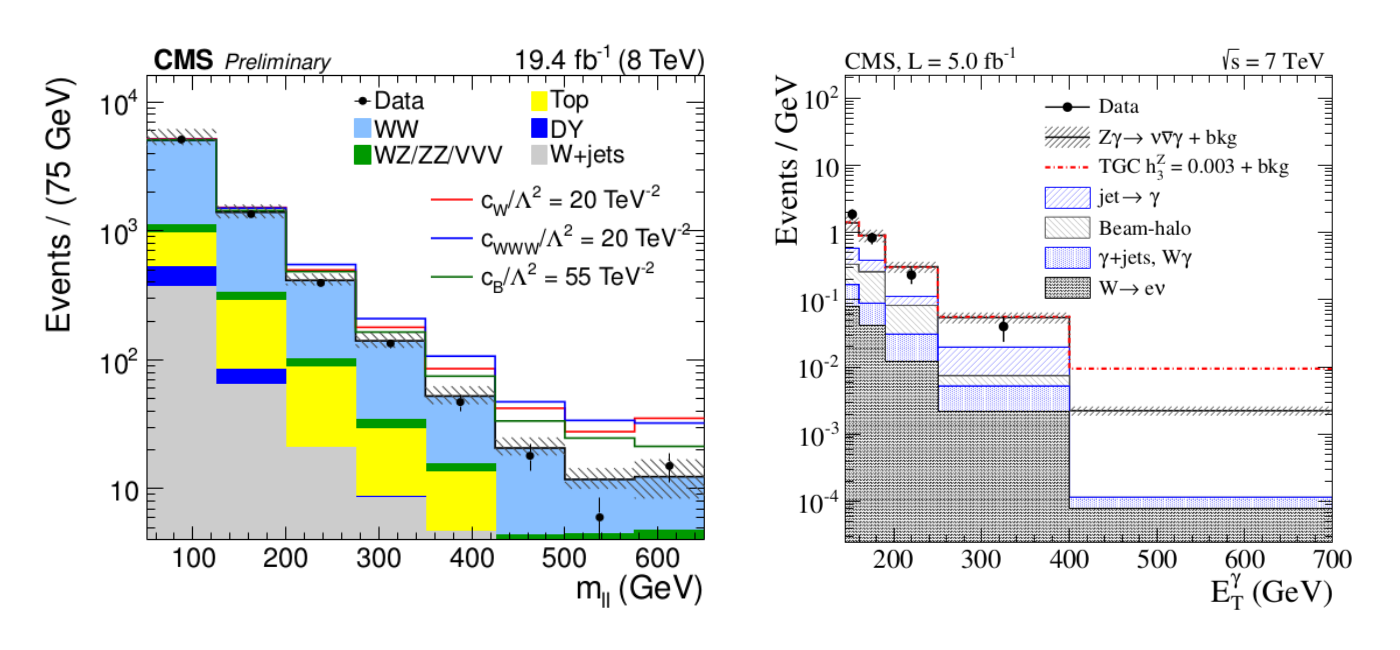
\includegraphics[width=0.85\textwidth]{../figs/WgAbout/aTGC_Pt_Examples.png}}
    \caption{Examples of the possible effects of non-zero TGC constants in $m_{ll}$ spectrum in 8 TeV $WW \rightarrow l\nu l\nu$ measurement (left) and $P_T^{\gamma}$ spectrum in 7 TeV $Z\gamma \rightarrow \nu\nu\gamma$ measurement (right).}
    \label{fig:aTGC_Pt_Examples}
  \end{center}
\end{figure}



\subsection{Measurements in the Past}
\label{sec:WgAbout_PastMeas}

ATGC parameters of $WW\gamma$ vertex can be probed in measurements of $W\gamma$, $WW$, $WZ$ processes. Limits on $\Delta \kappa_\gamma$ and $\lambda_\gamma$ constants obtained by different experiments are summarized in Fig.~\ref{fig:aTGC_cg}. The summary include the combination results from D0~\cite{ref_D0_aTGC_comb} ans LEP~\cite{ref_LEP_aTGC_comb} as well as results of several individual measurements by ATLAS~\cite{ref_7TeV_ATLAS},~\cite{ref_ATLAS_WW_8TeV},~\cite{ref_ATLAS_VW_8TeV} and CMS~\cite{ref_7TeV_CMS},~\cite{ref_CMS_WW_7TeV},~\cite{ref_CMS_WW_8TeV},~\cite{ref_CMS_VW_7TeV}.\\ 

\begin{figure}[htb]
  \begin{center}
    {\includegraphics[width=0.80\textwidth]{../figs/WgAbout/aTGC_cg.png}}
    \caption{Summary of limits on the $WW\gamma$ aTGC coupling constants. Figure from~\cite{ref_twiki_SMP_ATGC}.}
    \label{fig:aTGC_cg}
  \end{center}
\end{figure}

The most recent measurements of $W\gamma$ production were performed by CMS~\cite{ref_7TeV_CMS} and ATLAS~\cite{ref_7TeV_ATLAS} collaborations with $pp$ collisions at $\sqrt{s}=7$~GeV collected in~2011. Both collaborations considered two channels: $W\gamma\rightarrow\mu\nu\gamma$ and $W\gamma\rightarrow e\nu\gamma$.\\

%The measurements are based on~5~fb$^{-1}$ and~4.6~fb$^{-1}$ of integrated luminosity with CMS and ATLAS respectively.

Dibosons processes are rare in $pp$-collisions and analysts have to filter out events of their interest from many processes which are more likely to happen. To do that, variety of selection criteria is applied which reject most of background events increasing a signal fraction in the selected sample  as much as possible. However, even after all possible selection criteria are applied, majority of selected events are still background events and it is not possible to reduce the background any further without also significantly reducing signal.\\

The major source of such irreducible background is the fake photon background where hadronic jets are misidentified as photons. Such events originate from mostly $W+$jets process but $Z+$jets and $\bar{t}t+$jets events contribute to this source of the background as well. In the electron channel there is one more significant background that is the fake photon background where electron is misidentified as a photon.  Such events are coming from $Z+$jets events. For the muon channles this background is small.  Other sources of backgrounds for both channels include real-$\gamma$ backgrounds, fake lepton + real photon and fake lepton + fake photon sources.\\

Both channels provide measurements of $P_T^\gamma$ spectra because this variable is the most sensitive to the potential aTGC. The $P_T^\gamma$ spectra of the selected events in data superimposed with selected events in the simulation of the signal and estimated background contribution for the muon and electron channels are shown in Fig.~\ref{fig:Wg7TeV_CMS_ptGamma} for CMS and in Fig.~\ref{fig:Wg7TeV_ATLAS_ptGamma} for ATLAS. Both measurements show a good agreement between data and the simulation.\\

%To derive aTGC limits...

\begin{figure}[htb]
  \begin{center}
    {\includegraphics[width=0.80\textwidth]{../figs/WgAbout/Wg7TeV_CMS_ptGamma.png}}
    \caption{The distribution fo the $p_T^\gamma$ of W$\gamma$ candidates in the analysis of~7~TeV CMS data. Data vs signal MC + background estimates. Left: $W\gamma\rightarrow e\nu\gamma$, right: $W\gamma\rightarrow \mu\nu\gamma$~\cite{ref_7TeV_CMS}.}
    \label{fig:Wg7TeV_CMS_ptGamma}
  \end{center}
\end{figure}

\begin{figure}[htb]
  \begin{center}
    {\includegraphics[width=0.80\textwidth]{../figs/WgAbout/Wg7TeV_ATLAS_ptGamma.png}}
    \caption{The distribution of the photon transverse momentum (left) and missing transverse momentum (right) of W$\gamma$ candidates in the analysis of 7 TeV ATLAS data. Data vs signal MC + background estimates~\cite{ref_7TeV_ATLAS}. }
    \label{fig:Wg7TeV_ATLAS_ptGamma}
  \end{center}
\end{figure}

CMS provides measurements of the $P_T^\gamma$ spectrum, the total cross section within the phase spaces of $\Delta R>0.7$, $P_T^\gamma>15$~GeV, $P_T^\gamma>60$~GeV and $P_T^\gamma>90$~GeV, and limits on aTGC coupling constants. The phase space restrictions come from the considerations of the detector acceptance, reducing heavily background-dominated regions and theory.\\

ATLAS, in addition to the $P_T^\gamma$ spectrum, total cross section and limits, provides the differential cross section and cross section with different number of associated jets. No evidence of a new physics is observed.\\

In this dissertation we are measuring total and differential $d\sigma/d P_T^\gamma$ cross section. While the aTGC limits are not derived in this dissertation, the measured differential cross section can be used to derive them. The measurement details and results are described in Chapter~\ref{sec:AN_WgMeas}.\\


\chapter{Experimental Setup} % 7-20 pages
\label{sec:Exp}

The measurement reported in this dissertation is based on data collected by the CMS detector from the LHC $pp$~collisions in~2012. Thus, the experimental setup for this measurement includes the LHC and the CMS detector that are described in Ch.~\ref{sec:Exp_LHC} and Ch.~\ref{sec:Exp_CMS} respectively. 

% 7-20 pages
\subsection{Large Hadron Colllider}
main ring
injector
collision points
detectors (CMS, ATLAS, LHCb, ALICE)
list and briefly main discoveries 

Bunch crossing

\begin{figure}[htb]
  \begin{center}
    {\includegraphics[width=0.98\textwidth]{../figs/Exp/CERN_accelerator_complex2013.jpg}}
    \caption{CERN's accelerator complex. Source of the figure: \cite{ref_fig_CERNacceleratorComplex}.}
    \label{fig:SMtable}
  \end{center}
\end{figure}

\begin{figure}[htb]
  \begin{center}
    {\includegraphics[width=0.5\textwidth]{../figs/Exp/LHC_lumi.png}}
    \caption{LHC integrated luminosity by year. Source of the figure: \cite{ref_fig_LHClumi}.}
    \label{fig:SMtable}
  \end{center}
\end{figure}



\subsection{Compact Muon Solenoid}
\label{sec:Exp_CMS}
\subsubsection{Introduction}

CMS detector configuration
r-phi plane, r-z plane
slice in r-phi plane
subsystems
a particle traveling through the detector:
ele, pho, muon, hadron, neutrino
Where to place particle reconstruction, particle flow algorithm and MET? Check other theses
Acceptance: particles which are too collinear and go to pipe; particles which get curved too strongly

\subsubsection{CMS Magnet}
4T inside, 2T outside, needed for track curvatures to measure the momenta
need stronger field inside to distinguish tracks better, the track density in the tracker is much higher than in the muon system
explain how the magnetic field outside the detector is created
the size, what's inside, what's outside
material

\subsubsection{CMS Tracking System}
measures track geometry and momentum of charged particle
needs to disturb particles as little as possible: just a few measurement points to reconstruct the track
electric charge and amplification
silicon pixels, barrel and forward
silicon strips, barrel and forward
tracker alignment (here ?)
limitations

\subsubsection{CMS ECal}
measures energy of electrons and photons
also determines the track, especially for photons
match to tracker: if track, it's ele/pos, if not - it's a photon
(Why muons and hadrons don't release their energy here?)
electromagnetic shower
lead tungstate crystals
how scintillator works, what the scintillation light is
photodetectors (photomultipliers?)
ECAL preshower: to distinguish between two photons coming from pi0 decay
limitations

\subsubsection{CMS HCal}
measures energy of charged and neutral hadrons
also determines the track, especially for neutral hadrons
match to tracker: if track, it's charged, if not - it's neutral
(Why muons don't release their energy here? Would photons and electrons release the energy here?)
hadronic shower
HCal Sampling calorimeter (?)
Lqyers: absorber+scintillator
Hybrid Photodiodes

\subsubsection{CMS Muon System}
four layers of muon detectors (stations)
iron return yoke between them (how it works? why do we need it?)

>> (from cms.web.cern.ch) In total there are 1400 muon chambers: 250 drift tubes (DTs) and 540 cathode strip chambers (CSCs) track the particles’ positions and provide a trigger, while 610 resistive plate chambers (RPCs) form a redundant trigger system, which quickly decides to keep the acquired muon data or not. 

drift tubes
cathode strip chambers
resistive plate chambers

\subsubsection{Triggering and Data Aquisition}
Level-I trigger
High Level Trigger

\subsubsection{Event Reconstruction}



\chapter{CMS Tracker Alignment} % 5-10 pages
\label{sec:alignment}
A tracking system detects hits produced by a charged particle traveling through the detector that allows to reconstruct the full geometry of tack as well as determine a particle momentum. In a presence of a constant magnetic field the particle has a helical trajectory. A reconstruction algorithm determines the track parameters by fitting the positions of hits assuming the helical trajectory which can be defined by five parameters.

High precision track reconstruction is essencial for accurate analyses including particle identfication and measurements of kinematics. Better hit resolution and the location uncertainty lead to better precision of a measurement of the track parameters. The location uncertainty depends on our knowledge of the positions and orientations in space of the tracking system modules. The hit resolution in the CMS pixel detector is~$\sim$15~$\mu$m. When the modules are mounted, their positions are known with precision of~$\sim$200~$\mu$m. Thus, we need to know positions of modules~20~times better than they are known when mounted. The procedure of the determination of the modules locations and orientations is called the tracker alignment.


\subsection{Alignment Algorithm and Software}
Millepede, HIP, validation, CMSSW, configuration files

\subsection{Selected Results}
CRUZET, CRAFT and first collisions of 2015


\chapter{$W\gamma$ Cross Section Measurement}
\label{sec:AN_WgMeas}

The goal of the work reported in this dissertation is to measure the total and differential cross section of the $W\gamma$ production in $pp$ collisions as a function of the photon transverse momentum $P_T^\gamma$ at~$\sqrt{s}=$8~TeV center-of-mass collision energy. Decay channels $W\rightarrow\mu\nu$ and $W\rightarrow e\nu$ are considered. The measurement is performed using CMS data collected in~2012.

The phase space for the cross section was chosen taking into account the limitations on the event kinematics imposed by the trigger conditions during the data collection as well as by the detector acceptance, and considering the fact that the theoretical value for the cross section diverges at $P_T^{\gamma}=$0 and $\Delta{R}(\gamma,l)=$0. That phase space requirements on the final state photon and lepton match those of CMS $Z\gamma$ measurement at~8~TeV~\cite{ref_Zg8TeV} which also had to consider all the listed factors. The full list of the phase space requirements include:
%  Applied at generator-level to compute acceptance and MC-based cross section;\\
%  (tried to follow to the phase space definition of the approved Z$\gamma$ analysis [AN-2013-280] as close as possible)
\begin{itemize}
  \item $P_T^{\gamma}>$15 GeV;
  \item $\Delta{R}(\gamma,l) > $0.7;
  \item $|\eta^{\gamma}|<$2.5, $|\eta^{l}|<$2.5;
  \item $P_T^{l}>$20 GeV;
  \item $I^{\gamma}<$5 GeV, where $I_{\gamma}$ is a sum of $P_T$ of all particles $p$ in the event within $\Delta{R(p,\gamma)}<$0.3.
%  \item for Z$\gamma$ Check: M(lep,lep)$>$50 GeV
%  \item for differential cross section, $P_T^{\gamma}$ binning: $15-20-25-30-35-45-55-65-75-85-95-120-500$~GeV.
\end{itemize}
\noindent{$P_T^{\gamma}$ ranges (binning) for the differential cross section measurement was chosen to match the CMS $Z\gamma$ measurement. The $P_T^\gamma$ bin boundaries are 15-20-25-30-35-45-55-65-75-85-95-120-500~GeV.}
 % 30 pages
%% Explain analysis outline here
%\section{Data and Monte Carlo samples}
\label{sec:DataAndMC}

%\subsection{Data sample}
The data sample we use in this analysis was recorded by the CMS experiment 
in 2012 in the LHC pp collisions at 8 TeV. The data is collected by single electron ($p_T>27$~GeV, WP 80) 
and single muon ($p_T>24$~GeV, $|\eta|<2.1$) triggers,
given in Table~\ref{tab:triggers}. 
Only certified runs and luminosity sections are considered, which 
means that good functioning of all CMS sub-detectors is required.
The selection of the validated run and luminosity sections are obtained from the following official JSON file:
\begin{itemize}
\item{\small{Cert$\_$190456$-$208686$\_$8TeV$\_$22Jan2013ReReco$\_$Collisions12$\_$JSON.txt}}
\end{itemize}
 The total 
amount of data analyzed correspond to an integrated luminosity of 19.6~\fbinv.

\begin{table}[htbp]
  \begin{center}
 {\small
  \begin{tabular} {l|l|c}
\hline
  Data set & Trigger name & Description\\
  \hline \hline
  SingleElectron & HLT\_Ele27\_WP80*        & $p_T>27$~GeV, HLT WP80 quality cuts \\
  \hline
  SingleMuon & HLT\_IsoMu24\_eta2p1      & $p_T>24$~GeV, $|\eta|<2.1$, isolated muon \\
  \hline
  \end{tabular}
}
  \caption{Analysis triggers for data sample.\label{tab:triggers}}
  \end{center}
\end{table}

The dataset used for the analysis and the corresponding run ranges are 
listed in Table~\ref{tab:datasets}. All samples have been processed using the 
\texttt{CMSSW\_5\_3\_2} release.\\

Double muon and double electron datasets are used for data-driven background estimation to select $Z\gamma$ ISR and FSR events.\\

\begin{table}[]
  \begin{center}
  \begin{tabular}{r|r}
  \hline
  Dataset name & Run range \\
  \hline
  /SingleElectron/Run2012A-22Jan2013-v1/AOD   &  190456-193621           \\
  \hline
  /SingleElectron/Run2012B-22Jan2013-v1/AOD   &   193833-196531       \\
  \hline
  /SingleElectron/Run2012C-22Jan2013-v1/AOD & 198022-203746\\
  \hline
  /SingleElectron/Run2012D-22Jan2013-v1/AOD  & 203777-208686 \\
  \hline
  /SingleMuon/Run2012A-22Jan2013-v1/AOD   &  190456-193621           \\
  \hline
  /SingleMuon/Run2012B-22Jan2013-v1/AOD   &   193833-196531       \\
  \hline
  /SingleMuon/Run2012C-22Jan2013-v1/AOD & 198022-203746\\
  \hline
  /SingleMuon/Run2012D-22Jan2013-v1/AOD  & 203777-208686 \\
  
  \hline
  \hline
  \end{tabular}
  \end{center}
  \caption{Summary of data samples used and run ranges of applicability.}
  \label{tab:datasets}
\end{table}%
%\subsection{Monte Carlo samples}

All Monte Carlo (MC) samples considered in this analysis come from the official
``Summer12\_53X'' production.  Events from all samples were
reconstructed making use of a \texttt{CMSSW\_5\_3\_X} release version.
The simulated samples are reweighted to represent the distribution of the
number of pp interactions per bunch crossing (pile-up), as measured in
the data.



Information regarding signal and background simulated MC samples used for the analysis is given in 
Table~\ref{tab:mc_bkg_samples}.  
The corresponding leading order (LO), next-to-leading order (NLO),
 and next-to-next-leading order (NNLO) 
cross sections are also listed in Table~\ref{tab:mc_bkg_samples}.



\begin{table}[h]
  \scriptsize
  \begin{center}
    \caption{Summary of Monte Carlo background samples used.}
    \begin{tabular}{|l|l|l|}
      \hline
      Process (Summer12)                     & $\sigma$, pb        & Dataset Name (AODSIM data tier) \\ \hline
      $W\gamma \rightarrow l\nu\gamma$     & 553.92 (NLO)         & \verb /WGToLNuG_TuneZ2star_8TeV-madgraph-tauola \\
      $W \rightarrow l\nu + jets$          & 36257.2 (NNLO)        & \verb /WJetsToLNu_TuneZ2Star_8TeV-madgraph-tarball \\ 
      $Z \rightarrow ll + jets$            & 3503.71         & \verb /DYJetsToLL_M-50_TuneZ2Star_8TeV-madgraph-tarball \\
      $t\bar{t} + jets+1l$                    & 99.44 (NNLO)          & \verb /TTJets_SemiLeptMGDecays_8TeV-madgraph  \\
      $t\bar{t} + jets+2l$                    & 23.83           & \verb /TTJets_FullLeptMGDecays_8TeV-madgraph \\
      $t\bar{t} + \gamma$                    & 1.444           & \verb /TTGJets_8TeV-madgraph \\
      $Z\gamma \rightarrow ll\gamma$       & 171.62          & \verb /ZGToLLG_8TeV-madgraph \\
      \hline
    \end{tabular}
    \label{tab:mc_bkg_samples}
  \end{center}
\end{table} 

The NLO cross section of W$\gamma$ was calculated with the MCFM in the same phase space for which the W$\gamma$ sample was generated. The theoretical computations of the NNLO cross section are available ~\cite{WgNNLOtheory} and its contribution is 19\%-26\%.\\

The cross section of Zg was computed using as inputs MCFM cross section values as well as the precise CMS measurementt~\cite{Zg8TeV} using the following procedure. The Z$\gamma$ cross section of $\sigma = 2073 \pm 95 \pm \11 \pm \53$ fb has been quoted in the phase space described in ~\cite{Zg8TeV}. To determine the measured cross section in the generator phase space, the following formula was used:\\
$\sigma_{narrow phase space}^{meas.}/\sigma_{wide phase space}^{meas.} = \sigma_{narrow phase space}^{MCFM}/\sigma_{wide phase space}^{MCFM}$.\\
The $\sigma_{narrow phase space}^{MCFM}$ was determined by computing how many events are falling into the narrow phase space and scaling it to $\sigma_{wide phase space}^{MCFM}$=159.12 pb. The $\sigma_{narrow phase space}^{MCFM}$ was found to be 1933 fb and 1911 fb for the muon and electron channels respectively and the average of 1922 fb was used in the formula. The $\sigma_{wide phase space}^{meas.}$ was found to be 171.62 pb.

%\section{Event and Object Selection}
\label{sec:AN_Selection}

%In this chapter we document the electron, muon, and photon identification and isolation criteria, $E_T^{MET}$ criteria, and provide the results of comparing simulation with data.


\subsection{Event Level Selection}
\label{sec:AN_Selection_EventLevel}

In the final state of the $W\gamma\rightarrow l\nu\gamma$ process, there is a lepton, a photon, and a neutrino. Because of that, we select events with exactly one lepton (muon or electron), a photon, both originating from the primary vertex, and with the significant missing transverse energy $E_T^{miss}$. The selection criteria for the individual electrons, muons and photons are described in Ch.~\ref{sec:AN_ObjectSelection}.

To select events with significant $E_T^{miss}$, we introduce a selection requirement on the transverse mass of a $W$~boson $M_T^W$ which is related to $E_T^{miss}$ as: 
\begin{equation}
M_T^W=\sqrt{(2  P_T^{l}  E_T^{miss}  (1-\cos{(\phi^{l}-\phi^{miss})}))},
\end{equation}
\noindent{where $P_T^l$ is a lepton transverse momentum, $\phi^{l}$ is an azimuthal angle of the lepton momentum, and $\phi^{miss}$ is an azimuthal angle of the missing transverse momentum. The requirement is $M_T^W>40$~GeV. The $M_T^W$ distribution is shown in Fig.~\ref{fig:DATAvsMC_WMt}. Photons with $P_T^{\gamma}<45$~GeV are selected for this plot because for such photons we do not expect them to be result of a new physics process.}

After the listed selection criteria are applied, significant background from DY+jets in the electron channel remains. This background is caused by one of the electrons misidentified as a photon. Its contribution is the most significant around the invariant mass of the electron-photon system $M_{e\gamma}$ close to the mass of the $Z$ boson (Fig.~\ref{fig:DATAvsMC_Mpholep1})because the distribution of $M_{ee}$ in the $Z\rightarrow e e$ decay is peaking at the value of the Z boson mass. To reduce this background, we apply $Z$-mass window selection criterion, more specifically, events with $70$~GeV$<M_{e\gamma}<110$~GeV are rejected. 

Finally, the separation $\Delta R=\sqrt{({\Delta\phi}^2+{\Delta\eta}^2)}$ between the final state lepton and photon is required to be $\Delta R(l,\gamma)>0.7$ to enhance the TGC contribution. In case if there is more than one photon in the selected event, the candidate with the photon of the highest~$P_T^{\gamma}$ is selected. 

Data and MC in Fig.~\ref{fig:DATAvsMC_WMt}-\ref{fig:DATAvsMC_Mpholep1} significantly disagree. Thus, a data-driven method is necessary to estimate the backgrounds.

\begin{figure}[htb]
  \begin{center}
   \includegraphics[width=0.5\textwidth]{../figs/figs_v11/MUON_WGamma/PrepareYields/c_TotalDATAvsMC_EtaCommon__WMtVERY_PRELIMINARY.pdf}\includegraphics[width=0.5\textwidth]{../figs/figs_v11/ELECTRON_WGamma/PrepareYields/c_TotalDATAvsMC_EtaCommon__WMtVERY_PRELIMINARY.pdf}
  \caption{ $M_T^W$ of $W\gamma$ candidates. Data vs MC plots. Left: muon channel, right: electron channel. All selection criteria except $M_{T}^W$ cut are applied on these plots. $15$~GeV$<P_T^{\gamma}<45$~GeV. }
  \label{fig:DATAvsMC_WMt}
  \end{center}
\end{figure}

\begin{figure}[htb]
  \begin{center}
   \includegraphics[width=0.5\textwidth]{../figs/figs_v11/MUON_WGamma/PrepareYields/c_TotalDATAvsMC_EtaCommon__Mpholep1_pt15to500_.pdf}\includegraphics[width=0.5\textwidth]{../figs/figs_v11/ELECTRON_WGamma/PrepareYields/c_TotalDATAvsMC_EtaCommon__Mpholep1PRELIMINARY_FOR_E_TO_GAMMA_WITH_PSV_CUT_pt15to500_.pdf}
  \caption{$M_{l\gamma}$ of $W\gamma$ candidates. Data vs MC plots. Left: muon channel, right: electron channel. All selection criteria except $M_{l\gamma}$ cut are applied on these plots. $P_T^{\gamma}>15$~GeV. }
  \label{fig:DATAvsMC_Mpholep1}
  \end{center}
\end{figure}

\subsection{Object Selection}
\label{sec:AN_ObjectSelection}

We select events with a muon and a photon in the final state for the muon channel and events with an electron and a photon in the final state for the electron channel. 

We apply selection requirements on transverse momenta of $P_T^{\mu}>25$ GeV on muons,  $P_T^e>30$~GeV on electrons and $P_T^{\gamma}>15$~GeV on photons. In addition, electrons and photons must be within barrel (EB) or endcap (EE) sections of the Ecal which correspondto pseudorapidity ranges of $|\eta^{e,\gamma}| < 1.4442$ and $1.566 < |\eta^{e,\gamma}| < 2.5$, respectively. Muons must be within $|\eta^{\mu}|<2.1$. Selection requirements on $P_T^{\mu}$, $\eta^{\mu}$, and $P_T^e$ are determined by the trigger requirements, $\eta^{e,\gamma}$ criteria are determined by the geometrical limitations of the detector acceptance, and $P_T^{\gamma}>15$~GeV is the phase space requirement.

CMS Particle Object Group (POG) provides their recommendations for object identification~(ID) criteria for any given period of data collection. Recommendations for~2012 data include two sets of muon~ID criteria: "Tight" and "Loose" and four sets of electron and photon~ID criteria: "Tight", "Medium", "Loose" and "Veto".

For muon selection, we apply "Tight"~ID criteria. We consider electrons passing the "Tight" ID criteria and photons passing the modified "Medium" ID criteria. The modification of the photons ID criteria was studied in the $W\gamma\gamma \rightarrow l\nu\gamma\gamma$ measurement~\cite{ref_Wgg8TeV}.  %No restrictions on the maximum number of the final state photons are applied, however, 

To reduce backgrounds from the process with two or more leptons, such as $Z\gamma\rightarrow l l \gamma$ process, in the muon channel, we reject all events that have the second reconstructed muon candidate with $P_T^{\mu}>10$ GeV and $|\eta|^{\mu}<2.4$, and in the electron channel, we reject events which have the second reconstructed electron candidate with $p_T^e>10$ GeV and satisfying the "Veto"~ID criteria.

Selection criteria are applied consistently on the data sample as well as on all MC samples. The selection efficiency may differ between data and MC. The ratios data and MC efficiencies are called the scale factors. The scale factors for the selection criteria recommended are provided by CMS POG. For the modified photon~ID criteria, the appropriate changes to the POG-recommended scale factors were applied derived by the $W\gamma\gamma$ team~\cite{ref_Wgg8TeV}.

% NEED PLOTS WITH SCALE FACTORS 


\subsection{Selected Events}

%Distributions of $P_T^{\gamma}$ and $M_T^W$ of the selected events are shown in Fig. \ref{fig:DATAvsMC} and \ref{fig:DATAvsMC_WMt}. 
%The is a large discrepancies in all the distributions and therefore the data-driven background estimates are necessary.\\

At the instantaneous luminosities of LHC in~2012, as a rule, multiple $pp$ interactions occured per bunch crossings. Multiple interactions are also simulated in the MC samples. However, MC samples are usually produced before data collection is finished, and in the end have to be rewithed so that the distribution of the number of interactions in simulated sample matches the data.

The pileup (PU) weights are assigned on each event in each MC sample. Figure~\ref{fig:DATAvsMC_nVtx} shows the distribution of the number of vertices of the $Z\gamma$-selected dataset overlaid with $Z\gamma$ and DY+jets MC samples in the muon channel before (left) and after (right) the PU reweighting of the MC samples. The $Z\gamma$-selected dataset is composed mainly of two sources and the $Z\gamma$ cross section is already measured and published by CMS~\cite{ref_Zg8TeV}, thus, we understand the distributions of $Z\gamma$-selected samples better the distributions of the $W\gamma$-selected samples. Thus, we use $Z\gamma$-selected dataset to validate the procedure of PU reweighting which is the same for $Z\gamma$-selected and $W\gamma$-selected MC samples.

\begin{figure}[htb]
  \begin{center}
   \includegraphics[width=0.45\textwidth]{../figs/figs_v11/MUON_ZGamma/PrepareYields/c_TotalDATAvsMC_EtaCommon__nVtx_noPU.png}\includegraphics[width=0.45\textwidth]{../figs/figs_v11/MUON_ZGamma/PrepareYields/c_TotalDATAvsMC_EtaCommon__nVtx.png}
  \caption{Number of vertices of $Z\gamma$ candidates in the muon channel. Data vs MC. Left: no PU reweighting applied, right: PU reweighting applied. }
  \label{fig:DATAvsMC_nVtx}
  \end{center}
\end{figure}

$W$+jets, DY+jets and $t\bar{t}$+jets MC samples partially contain $W\gamma$, $Z\gamma$, and $t\bar{t}\gamma$ events. The overlap was removed from the $W$+jets, DY+jets, and $t\bar{t}$+jets samples relying on their gen-level information. A good data vs MC agreement for the $Z\gamma$ plots in Fig.~\ref{fig:DATAvsMC_nVtx} validates the procedure of the overlap removal.

Distributions of $P_T^{\gamma}$ of the selected events are shown in Fig.~\ref{fig:DATAvsMC}. The are large discrepancies in all the distributions and therefore the data-driven background estimates are necessary.

\begin{figure}[htb]
  \begin{center}
   \includegraphics[width=0.45\textwidth]{../figs/figs_v11/MUON_WGamma/PrepareYields/c_TotalDATAvsMC_Barrel__phoEt.pdf}\includegraphics[width=0.45\textwidth]{../figs/figs_v11/ELECTRON_WGamma/PrepareYields/c_TotalDATAvsMC_Barrel__phoEt.pdf}
   \includegraphics[width=0.45\textwidth]{../figs/figs_v11/MUON_WGamma/PrepareYields/c_TotalDATAvsMC_Endcap__phoEt.pdf}\includegraphics[width=0.45\textwidth]{../figs/figs_v11/ELECTRON_WGamma/PrepareYields/c_TotalDATAvsMC_Endcap__phoEt.pdf}
  \caption{$P_T^{\gamma}$ of $W\gamma$ candidates. Data vs MC plots. Left column: muon channel, right column: electron channel. Top to bottom: photons in EB and EE of ECal.}
  \label{fig:DATAvsMC}
  \end{center}
\end{figure}



%\begin{figure}[htb]
%  \begin{center}
%   \includegraphics[width=0.45\textwidth]{figs_v8/MUON_WGamma/PrepareYields/c_TotalDATAvsMC_Barrel__WMtVERY_PRELIMINARY.pdf}\includegraphics[width=0.45\textwidth]{figs_v8/ELECTRON_WGamma/PrepareYields/c_TotalDATAvsMC_Barrel__WMtVERY_PRELIMINARY.pdf}
%   \includegraphics[width=0.45\textwidth]{figs_v8/MUON_WGamma/PrepareYields/c_TotalDATAvsMC_Endcap__WMtVERY_PRELIMINARY.pdf}\includegraphics[width=0.45\textwidth]{figs_v8/ELECTRON_WGamma/PrepareYields/c_TotalDATAvsMC_Endcap__WMtVERY_PRELIMINARY.pdf}
%  \caption{Data vs MC plots, $M_T^W$. Left column - muon channel, right column - electron. Top to bottom: barrel and endcap photons. All selection criteria except $M_T^W$ cut on these plots. $15$~GeV$<P_T^{\gamma}<45$~GeV. The analysis cut of $M_T^W>40$~GeV is selected.}
%  \label{fig:DATAvsMC_WMt}
%  \end{center}
%\end{figure}

%\section{Background Subtraction}
\label{sec:BackgroundSubtraction}

The selected sample contains signal events as well as events coming from various backgrounds. To compute the cross section, we need to subtract background and estimate how many events in each $P_T^\gamma$ bin originate from the $W\gamma$ process. This chapter describes the methods used for the background subtraction and provides the results.

\subsection{Jets$\rightarrow\gamma$ Background Estimation and Subtraction}
\label{sec:BackgroundSubtraction_jtog}

The selected sample is dominated by the $W$+jets background which cannot be further significantly reduced without reducing our signal sample $W\gamma$ as well. The photon~ID selection criteria help to reduce $W$+jets background to a certain level but there is still a significant number of jets that are reconstructed as photons and pass all the photon~ID criteria. DY+jets is another source of the jets$\rightarrow \gamma$ background but this source is significantly suppressed by the $M_W^T$ selection criterion in both channels and by the $Z$-mass window requirement in the electron channel.

The template method is used to estimate jets$ \rightarrow \gamma$ background. First of all, we choose a variable that has a significant discriminative power between the true and fake photon candidates $V_{fit}$. After that, we prepare real-$\gamma$ ($T_{true}$) and fake-$\gamma$ ($T_{fake}$) templates which should be an accurate representations of $V_{fit}$ distributions of real and fake photons in the $W\gamma$-selected dataset. The $V_{fit}$ distribution in data is fitted by the following function: 
\begin{equation}
F(V_{fit})=N_{true} \cdot T_{true}(V_{fit}) + N_{fake} \cdot T_{fake}(V_{fit}),
\end{equation}
\noindent{where $V_{fit}$ is a fit variable, $N_{true}$ and $N_{fake}$ are numbers of real and fake photons in the data sample, respectively, and $F(V_{fit})$ is a fit function. $N_{true}$ and $N_{fake}$ are fit parameters. We use the charged hadron isolation $I_{ch}^{\gamma}$ and a shower shape variable $\sigma_{i\eta i\eta}^{\gamma}$ as $V_{fit}$. Results of $I_{ch}^{\gamma}$ fits are further propagated for the cross section calculation, and results of $\sigma_{i\eta i\eta}^{\gamma}$ fits are used for the estimation of the systematic uncertainty.}

% EXPLAIN WHAT IS I_{CH}^{\gamma} and WHAT IS SIHIH
The $I_{ch}^{\gamma}$ is defined as
\begin{equation}
  I_{ch}^{\gamma} = \sum_{ch} P_T,
\end{equation} 
\noindent{where the sum runs over charged hadrons candidates reconstructed by the particle flow algorithm within $\Delta R<0.3$ from the photon.}

The $\sigma_{i\eta i\eta}^{\gamma}$ is defined as
\begin{equation}
  \sigma_{i\eta i\eta}^{\gamma} = \frac{\sum{(\eta_i-\eta)^2 w_i}}{\sum(w_i)},
\end{equation}
\noindent{where the sum runs over~$5\times5$ matrix of crystals around the crystal with the largest $P_T$, and $w_i$ is the weight that has a logarithmic dependence on energy released by the photon.}

To prepare templates, we use $Z\gamma$-selected dataset. $Z\gamma$ goes through two different mechanisms: FSR, when a photon is radiated from one of the final state leptons, and ISR, when a photon is radiated from the initial state quark or antiquark. Real-$\gamma$ templates $T_{true}$ are taken from the FSR events of $Z\gamma\rightarrow\mu\mu\gamma$ while fake-$\gamma$ templates are taken from the ISR events of $Z\gamma\rightarrow\mu\mu\gamma$.

The FSR $Z\gamma$ selection has muon-photon separation requirement of $\Delta R_{min}(\mu,\gamma)>0.4$. This requirement is chosen to be smaller than nominal separation requirement of $\Delta R_{min}(\mu,\gamma)>0.7$ because FSR events typically have smaller separation than ISR events and, therefore, smaller separation increases a fraction of FSR events. Three-particle invariant mass required to be $M_{\gamma\mu\mu}<101$~GeV. 

The FSR contribution drops fast as a function of $P_{T}^{\gamma}$, therefore, the FSR sample has a small statistical power in high $P_{T}^{\gamma}$ bins. To increase the statistical power, we use events from several $P_T^{\gamma}$ ranges to prepare templates for each of them. The distribution of $I_{ch}^{\gamma}$ of real photons does not depend on $P_{T}^{\gamma}$ and, therefore, all events with $P_{T}^{\gamma}>15$~GeV are used to prepare $I_{ch}^{\gamma}$ templates for all $P_T^{\gamma}$ bins. Distributions of $\sigma_{i\eta i\eta}^{\gamma}$ depend on $P_T^{\gamma}$. Only events of $P_T^{\gamma}>30$~GeV are merged together to prepare templates for all $P_T^{\gamma}>30$~GeV bins. Both $I_{ch}^{\gamma}$ and $\sigma_{i\eta i\eta}^{\gamma}$ templates are prepared separately for barrel and endcap photons.

To prepare fake-$\gamma$ templates, we need a sample that consists of jets reconstructed and identified as photons. To prepare such sample, we apply ISR $Z\gamma$ selection conditions on double muon dataset. These selection conditions include nominal $Z\gamma$ selection described in Ch.~\ref{sec:AN_ObjectID} with tighter requirement on the lepton-photon separation $\Delta{R_{min}}(\mu,\gamma)>1.0$, and a requirement on the invariant mass of the three final satte particles $M_{ll\gamma}>101$~GeV. A sample prepared in such a way consists of $Z\gamma$+(DY+jets) events, and jets from the DY+jets are reconstructed and identified as photons same as jets from $W$+jets, DY+jets and $t\bar{t}$+jets in a $W\gamma$-selected sample. 

Therefore, to construct a fake-$\gamma$ template, we can use DY+jets events from the ISR $Z\gamma$-selected sample. However, in addition to DY+jets events, this sample also contains non-negligible amount of $Z\gamma$ events. This real-$\gamma$ contribution is subtracted using $Z\gamma$ MC predictions.

FSR and ISR selections are illustrated in App.~\ref{sec:ZgFSRandISRplots}. Distributions of $M_{ll\gamma}$ and $M_{ll}$ for nominally selected $Z\gamma$ dataset are shown in Fig.~\ref{fig:Zg_Mleplep_and_Mpholeplep}. Distributions of $\Delta{R}(l,\gamma)$ for ISR and FSR $Z\gamma$ events are shown in Fig.~\ref{fig:Zg_ISRandFSR_dR}. Distributions of $P_{T}^{\gamma}$ for ISR and FSR $Z\gamma$ events are shown in Fig.~\ref{fig:Zg_ISRandFSR_phoEt}. High $P_{T}^{\gamma}$ bins have higher real-$\gamma$ contamination but even the last bin contains enough events to prepare a template. 

Fits are performed in the extended binned maximum likelihood manner separately in each $P_T^{\gamma}$ bin, separately for EB and EE photons. Plots of the template fits are available in App.~\ref{sec:TemplateFitPlots}.   

To extract real-$\gamma$ yield from the $N_{true}$, efficiency of the $V_{fit}$ is applied on the value derived from fit based on the distribution of events which are used to prepare the real-$\gamma$ template. To extract fake-$\gamma$ yield from the $N_{fake}$, efficiency of the $V_{fit}$ is applied on the value derived from fit based on the distribution of events which are used to prepare a fake-$\gamma$ template. 

Two MC closure checks are performed to validate the procedure. For the first check all MC samples that pass $W\gamma$ selection are mixed together with appropriate weights assigned. Then fits on this sample of pseudodata are performed as on real data and the fit results are superimposed with MC samples. The results of the MC closure check are reported in App.~\ref{sec:MCclosureCheck} and the fit plots are shown in App.~\ref{sec:TemplateFitPlotsMCclosure}. 

For the second MC closure check, the pseudodata sample is prepared from $W$+jets and $W\gamma$ samples only. The results are reported in App.~\ref{sec:TemplateFitPlotsMCclosureWjetsPlusWg}. 

\subsection{$e\rightarrow\gamma$ Background Estimation and Subtraction for the Electron Channel}
\label{sec:BackgroundSubtraction_etog}

For the electron channel, DY+jets is the main source of the $e \rightarrow \gamma$ background. The $Z$-mass window requirement of ($M_{e\gamma}<70$~GeV or $M_{e\gamma}>110$~GeV) significantly suppresses this background, however, the remaining contribution is non-negligible. 

The contribution of $e\rightarrow\gamma$ is estimated separately for each $P_{T}^{\gamma}$ bin and separately for barrel and endcap photons using the following expression: 

\begin{equation}
N_{data-nom}^{e\rightarrow\gamma} = N_{MC-nom}^{e\rightarrow\gamma} \cdot \frac{N_{data-Zpeak}^{e\rightarrow\gamma}}{N_{MC-Zpeak}^{e\rightarrow\gamma}}, 
\end{equation}
\noindent{where $N_{data-nom}^{e\rightarrow\gamma}$ and $N_{MC-nom}^{e\rightarrow\gamma}$ are the numbers of $e\rightarrow\gamma$ events in the nominally selected of data and DY+jets MC sample, respectively, $N_{data-Zpeak}^{e\rightarrow\gamma}$ and $N_{MC-Zpeak}^{e\rightarrow\gamma}$ are the numbers of $e\rightarrow\gamma$ events under the $Z$-peak data and DY+jets MC sample respectively. }

To estimate number of events under $Z$-peak, $e\rightarrow\gamma$-enriched data and DY+jets MC samples are prepared by inverting the $Z$-mass
window requirement. After that, numbers of events in DY+jets MC samples $N_{MC-Zpeak}^{e\rightarrow\gamma}$ and $N_{MC-nom}^{e\rightarrow\gamma}$ are estimated by counting with appropriate weights. The number $N_{data-Zpeak}^{e\rightarrow\gamma}$ is extracted from fitting the $M_{e\gamma}$ in the $Z$-peak region (App.~\ref{sec:EtogammaFitPlots}). The fits are performed separately in each $P_T^\gamma$ bin in fine $\eta^\gamma$ binning:
     \begin{itemize}
        \item $P_T^\gamma$ $15-20-25-30-35-45-55-65$~GeV
           \begin{itemize}
              \item $\eta^\gamma$ binning in barrel: $0.00-0.10-0.50-1.00-1.44$
              \item $\eta^\gamma$ binning in endcap: $1.56-2.10-2.20-2.40-2.50$
           \end{itemize}
        \item $P_T^\gamma$ $65-75-85-95$~GeV
          \begin{itemize}
              \item $\eta^\gamma$ binning in barrel: $0.00-0.50-1.44$
              \item $\eta^\gamma$ binning in endcap: $1.56-2.20-2.50$
           \end{itemize}
        \item $P_T^\gamma$: $95-120-500$~GeV
          \begin{itemize}
              \item $\eta^\gamma$ binning in barrel: $0.00-1.44$
              \item e$\eta^\gamma$ binning in ndcap: $1.56-2.50$
           \end{itemize}
        \item $P_T^\gamma$ $10-15$~GeV (underflow bin): MC-prediction is used, no fit performed.
     \end{itemize}
\noindent{The fit plots are provided in App.~\ref{sec:EtogammaFitPlots} and the tables are provided in App.~\ref{sec:etogTables}. To prepare yields, fit results in all fine barrel $\eta^\gamma$ bins are summed up and fit results in all fine endcap $\eta^\gamma$ bins are summed up. The distributions of $M_{e\gamma}$ before and after appropriate scale of the $e\rightarrow\gamma$ of the DY+jets sample is in different $P_T^{\gamma}$ bins are shown in App.~\ref{sec:Mpholep1DatavsMC}.}

%  \item templates for RooNDKeysPdf: $e\rightarrow\gamma$ portion of the DYjets MC separately for each pt-eta bin
%  \item $e\rightarrow\gamma$ portion of the DYjets MC: a photon has a gen-level electron within dR=0.4 


\subsection{Other Backgrounds}

In addition to the backgrounds discussed before, there is also real-$\gamma$ background. The contributions to this background from $Z\gamma$ and $W\gamma \rightarrow \tau \nu \gamma$ are estimated based on MC predictions.

\begin{itemize}
   \item real-$\gamma$ background from $WW\gamma$;  
   \item $e \rightarrow \gamma$ background in the muon channel. Sources of these backgrounds are $WW$ ($W \rightarrow \mu\nu_{\mu}$ + $W \rightarrow e\nu_e$), $WZ$ ($W \rightarrow \mu\nu_{\mu}$ + $Z \rightarrow ee$ or $W \rightarrow e\nu_{\mu}$ + $Z \rightarrow \mu\mu$) and $ZZ$ ($Z \rightarrow \mu\mu$ + $Z \rightarrow ee$);
   \item fake lepton + real-$\gamma$ ($\gamma$+jets and $\gamma\gamma$+jets events); 
   \item fake lepton + fake-$\gamma$ (multijets events).  
\end{itemize}

\subsection{$P_T^{\gamma}$ Spectra before and after the Background Subtraction}

The results of the background estimation and subtraction procedure are summarized in Fig.~\ref{fig:DDvsMC_Wg_Data_MUON}-\ref{fig:DDvsMC_Wg_Data_ELECTRON} and in Tab.~\ref{tab:yields_Wg_to_munu__Barrel_}-\ref{tab:yields_Wg_to_enu__Endcap_}. Figure~\ref{fig:DDvsMC_Wg_Data_MUON} and Tab.~\ref{tab:yields_Wg_to_munu__Barrel_}-~\ref{tab:yields_Wg_to_munu__Endcap_} stand for the muon channel while Fig.~\ref{fig:DDvsMC_Wg_Data_ELECTRON} and Tab.~\ref{tab:yields_Wg_to_enu__Barrel_}-\ref{tab:yields_Wg_to_enu__Endcap_} stand for the electron channel. Top and middle plots in Fig.~\ref{fig:DDvsMC_Wg_Data_MUON}-\ref{fig:DDvsMC_Wg_Data_ELECTRON} shows the $P_T^\gamma$ spectrum in data superimposed with the signal MC and background estimates that includes jets$\rightarrow\gamma$ and real-$\gamma$ backgrounds in both channels and $e\rightarrow\gamma$ background in the electron channel. The bottom plots show data yields after full background subtraction superimposed with signal MC. 

Jets$\rightarrow\gamma$ background is estimated by two methods. The results provided by two methods differ significantly, and the difference contributes to the systematic uncertainty.

\begin{figure}[htb]
  \begin{center}
   \includegraphics[width=0.45\textwidth]{../figs/figs_v11/MUON_WGamma/PrepareYields/c_DATAvsBkgPlusSigMCc_MUON_WGamma_TEMPL_CHISO_UNblind__Barrel__phoEt.pdf}\includegraphics[width=0.45\textwidth]{../figs/figs_v11/MUON_WGamma/PrepareYields/c_DATAvsBkgPlusSigMCc_MUON_WGamma_TEMPL_SIHIH_UNblind__Barrel__phoEt.pdf}  \\
   \includegraphics[width=0.45\textwidth]{../figs/figs_v11/MUON_WGamma/PrepareYields/c_DATAvsBkgPlusSigMCc_MUON_WGamma_TEMPL_CHISO_UNblind__Endcap__phoEt.pdf}\includegraphics[width=0.45\textwidth]{../figs/figs_v11/MUON_WGamma/PrepareYields/c_DATAvsBkgPlusSigMCc_MUON_WGamma_TEMPL_SIHIH_UNblind__Endcap__phoEt.pdf}  \\
\includegraphics[width=0.45\textwidth]{../figs/figs_v11/MUON_WGamma/PrepareYields/c_BkgSubtrDATAvsSIGMC_c_MUON_WGamma__UNblind__Barrel__phoEt.pdf}\includegraphics[width=0.45\textwidth]{../figs/figs_v11/MUON_WGamma/PrepareYields/c_BkgSubtrDATAvsSIGMC_c_MUON_WGamma__UNblind__Endcap__phoEt.pdf}\\
  \caption{Top and middle: data vs fake-$\gamma$ background derived from the template method + real-$\gamma$ background predicted by dedicated MC samples + signal MC, with $I_{ch}$ and $\sigma_{i\etai\eta}$ used as fit variables. Bottom: data yields after full background subtraction vs signal MC. $I_{ch}$ vs $\sigma_{i\etai\eta}$ fit results. Muon channel.}
  \label{fig:DDvsMC_Wg_Data_MUON}
  \end{center}
\end{figure}

\begin{figure}[htb]
  \begin{center}
   \includegraphics[width=0.45\textwidth]{../figs/figs_v11/ELECTRON_WGamma/PrepareYields/c_DATAvsBkgPlusSigMCc_ELECTRON_WGamma_TEMPL_CHISO_UNblind__Barrel__phoEt.pdf}\includegraphics[width=0.45\textwidth]{../figs/figs_v11/ELECTRON_WGamma/PrepareYields/c_DATAvsBkgPlusSigMCc_ELECTRON_WGamma_TEMPL_SIHIH_UNblind__Barrel__phoEt.pdf}  \\
   \includegraphics[width=0.45\textwidth]{../figs/figs_v11/ELECTRON_WGamma/PrepareYields/c_DATAvsBkgPlusSigMCc_ELECTRON_WGamma_TEMPL_CHISO_UNblind__Endcap__phoEt.pdf}\includegraphics[width=0.45\textwidth]{../figs/figs_v11/ELECTRON_WGamma/PrepareYields/c_DATAvsBkgPlusSigMCc_ELECTRON_WGamma_TEMPL_SIHIH_UNblind__Endcap__phoEt.pdf}  \\
\includegraphics[width=0.45\textwidth]{../figs/figs_v11/ELECTRON_WGamma/PrepareYields/c_BkgSubtrDATAvsSIGMC_c_ELECTRON_WGamma__UNblind__Barrel__phoEt.pdf}\includegraphics[width=0.45\textwidth]{../figs/figs_v11/ELECTRON_WGamma/PrepareYields/c_BkgSubtrDATAvsSIGMC_c_ELECTRON_WGamma__UNblind__Endcap__phoEt.pdf}\\
  \caption{Top and middle: data vs fake-$\gamma$ background derived from the template method + real-$\gamma$ background predicted by dedicated MC samples + signal MC, with $I_{ch}$ and $\sigma_{i\etai\eta}$ used as fit variables. Bottom: data yields after full background subtraction vs signal MC. $I_{ch}$ vs $\sigma_{i\etai\eta}$ fit results. Electron channel.}
  \label{fig:DDvsMC_Wg_Data_ELECTRON}
  \end{center}
\end{figure}

\clearpage

\begin{table}[h]
  \scriptsize
  \begin{center}
  \caption{Data, signal and background yields. $W\gamma$, muon channel, barrel photons.}
  \begin{tabular}{|c|c|c|c|c|c|c|}
    bin & data & jets$\rightarrow\gamma$ & jets$\rightarrow\gamma$ & MC real-$\gamma$ &  data-bkg & signal \\ 
    lims & & $I_{ch}^{\gamma}$ & $\sigma_{i\eta i\eta}^{\gamma}$ & bkg & & MC  \\ \hline
10-15 & 114047$\pm$338 & 79833$\pm$251 & 77612$\pm$322 & 2453$\pm$46 & 26867$\pm$385 & 26251$\pm$240 \\ \hline 
15-20 & 41411$\pm$203 & 21434$\pm$150 & 24543$\pm$143 & 1566$\pm$34 & 19642$\pm$245 & 12707$\pm$164 \\ \hline 
20-25 & 19801$\pm$141 & 8466$\pm$101 & 9878$\pm$78 & 1283$\pm$31 & 10446$\pm$168 & 6793$\pm$120 \\ \hline 
25-30 & 11409$\pm$107 & 3509$\pm$68 & 4402$\pm$46 & 1180$\pm$27 & 7180$\pm$123 & 4087$\pm$93 \\ \hline 
30-35 & 7717$\pm$88 & 1687$\pm$49 & 2944$\pm$40 & 1253$\pm$27 & 5181$\pm$99 & 2604$\pm$75 \\ \hline 
35-45 & 9339$\pm$97 & 1947$\pm$56 & 2540$\pm$33 & 1840$\pm$33 & 5587$\pm$114 & 2971$\pm$80 \\ \hline 
45-55 & 3950$\pm$63 & 731$\pm$40 & 1964$\pm$40 & 477$\pm$18 & 2923$\pm$75 & 1861$\pm$63 \\ \hline 
55-65 & 2172$\pm$47 & 415$\pm$25 & 363$\pm$11 & 164$\pm$12 & 1694$\pm$50 & 1135$\pm$50 \\ \hline 
65-75 & 1320$\pm$36 & 177$\pm$17 & 466$\pm$19 & 81$\pm$8 & 1106$\pm$39 & 664$\pm$38 \\ \hline 
75-85 & 899$\pm$30 & 103$\pm$13 & 238$\pm$16 & 51$\pm$7 & 773$\pm$32 & 452$\pm$31 \\ \hline 
85-95 & 600$\pm$24 & 76$\pm$11 & 146$\pm$11 & 34$\pm$6 & 510$\pm$26 & 341$\pm$27 \\ \hline 
95-120 & 856$\pm$29 & 67$\pm$11 & 319$\pm$25 & 60$\pm$9 & 750$\pm$31 & 454$\pm$31 \\ \hline 
120-500 & 897$\pm$30 & 28$\pm$7 & 83$\pm$7 & 50$\pm$8 & 825$\pm$31 & 547$\pm$34 \\ \hline 
  \end{tabular}
  \label{tab:yields_Wg_to_munu__Barrel_}
  \end{center}
\end{table}

\begin{table}[h]
  \scriptsize
  \begin{center}
  \caption{Data, signal and background yields. $W\gamma$, muon channel, endcap photons.}
  \begin{tabular}{|c|c|c|c|c|c|c|}
    bin & data & jets$\rightarrow\gamma$ & jets$\rightarrow\gamma$ & MC real-$\gamma$ &  data-bkg & signal \\ 
    lims & & $I_{ch}^{\gamma}$ & $\sigma_{i\eta i\eta}^{\gamma}$ & bkg & & MC  \\ \hline
10-15 & 94370$\pm$307 & 77649$\pm$215 & 81161$\pm$426 & 2632$\pm$41 & 7937$\pm$306 & 10823$\pm$154 \\ \hline 
15-20 & 34643$\pm$186 & 25902$\pm$142 & 27661$\pm$184 & 1835$\pm$34 & 5089$\pm$213 & 6474$\pm$120 \\ \hline 
20-25 & 15988$\pm$126 & 10018$\pm$93 & 11659$\pm$102 & 1294$\pm$29 & 4842$\pm$138 & 3377$\pm$86 \\ \hline 
25-30 & 8429$\pm$92 & 4061$\pm$58 & 4558$\pm$51 & 871$\pm$23 & 3460$\pm$98 & 2068$\pm$67 \\ \hline 
30-35 & 5110$\pm$71 & 2669$\pm$54 & 2268$\pm$32 & 641$\pm$19 & 1700$\pm$81 & 1404$\pm$56 \\ \hline 
35-45 & 5414$\pm$74 & 1807$\pm$44 & 2113$\pm$29 & 771$\pm$22 & 2957$\pm$83 & 1489$\pm$57 \\ \hline 
45-55 & 2422$\pm$49 & 1025$\pm$50 & 936$\pm$19 & 222$\pm$13 & 1196$\pm$68 & 819$\pm$43 \\ \hline 
55-65 & 1217$\pm$35 & 270$\pm$19 & 564$\pm$16 & 94$\pm$9 & 966$\pm$36 & 551$\pm$35 \\ \hline 
65-75 & 703$\pm$27 & 87$\pm$11 & 346$\pm$13 & 54$\pm$7 & 604$\pm$28 & 280$\pm$25 \\ \hline 
75-85 & 451$\pm$21 & 63$\pm$9 & 117$\pm$6 & 30$\pm$5 & 379$\pm$22 & 186$\pm$20 \\ \hline 
85-95 & 303$\pm$17 & 37$\pm$7 & 56$\pm$4 & 21$\pm$5 & 255$\pm$18 & 139$\pm$18 \\ \hline 
95-120 & 433$\pm$21 & 20$\pm$5 & -81$\pm$5 & 32$\pm$6 & 374$\pm$21 & 209$\pm$22 \\ \hline 
120-500 & 396$\pm$20 & 11$\pm$4 & 153$\pm$12 & 10$\pm$2 & 302$\pm$18 & 157$\pm$19 \\ \hline 
  \end{tabular}
  \label{tab:yields_Wg_to_munu__Endcap_}
  \end{center}
\end{table}

\clearpage

\begin{table}[h]
  \scriptsize
  \begin{center}
  \caption{Data, signal and background yields. $W\gamma$, electron channel, barrel photons.}
  \begin{tabular}{|c|c|c|c|c|c|c|c|}
    bin & data & jets$\rightarrow\gamma$ & jets$\rightarrow\gamma$ &  & MC real-$\gamma$ &  data-bkg & signal \\
    lims & & $I_{ch}^{\gamma}$ & $\sigma_{i\eta i\eta}^{\gamma}$ &$e\rightarrow\gamma$ & bkg & & MC  \\ \hline
10-15 & 71649$\pm$268 & 51004$\pm$200 & 53577$\pm$266 & 2923$\pm$80 & 2688$\pm$41 & 12425$\pm$316 & 12480$\pm$164 \\ \hline
15-20 & 25455$\pm$160 & 13487$\pm$118 & 14474$\pm$110 & 3715$\pm$178 & 1779$\pm$32 & 7422$\pm$262 & 5858$\pm$110 \\ \hline
20-25 & 11130$\pm$105 & 5112$\pm$78 & 4846$\pm$55 & 2023$\pm$137 & 1101$\pm$25 & 3168$\pm$186 & 2869$\pm$77 \\ \hline
25-30 & 5388$\pm$73 & 1748$\pm$47 & 1790$\pm$29 & 1031$\pm$72 & 603$\pm$18 & 2251$\pm$111 & 1412$\pm$54 \\ \hline
30-35 & 2907$\pm$54 & 752$\pm$32 & 1079$\pm$24 & 286$\pm$33 & 229$\pm$12 & 1831$\pm$68 & 916$\pm$44 \\ \hline
35-45 & 3128$\pm$56 & 735$\pm$34 & 1003$\pm$21 & 215$\pm$27 & 223$\pm$12 & 1965$\pm$70 & 1248$\pm$51 \\ \hline
45-55 & 2147$\pm$46 & 551$\pm$31 & 964$\pm$28 & 335$\pm$37 & 134$\pm$10 & 1200$\pm$65 & 821$\pm$42 \\ \hline
55-65 & 1556$\pm$39 & 228$\pm$19 & 211$\pm$8 & 272$\pm$39 & 108$\pm$9 & 1011$\pm$57 & 654$\pm$37 \\ \hline
65-75 & 1083$\pm$33 & 163$\pm$16 & 300$\pm$15 & 143$\pm$27 & 64$\pm$7 & 757$\pm$44 & 441$\pm$31 \\ \hline
75-85 & 680$\pm$26 & 79$\pm$11 & 224$\pm$15 & 45$\pm$13 & 62$\pm$7 & 516$\pm$31 & 295$\pm$26 \\ \hline
85-95 & 473$\pm$22 & 43$\pm$9 & 99$\pm$9 & 43$\pm$17 & 34$\pm$5 & 366$\pm$29 & 234$\pm$23 \\ \hline
95-120 & 703$\pm$27 & 53$\pm$9 & 274$\pm$24 & 63$\pm$19 & 47$\pm$5 & 555$\pm$34 & 318$\pm$27 \\ \hline
120-500 & 859$\pm$29 & 23$\pm$6 & 61$\pm$6 & 34$\pm$12 & 71$\pm$8 & 735$\pm$33 & 430$\pm$31 \\ \hline
  \end{tabular}

  \label{tab:yields_Wg_to_enu__Barrel_}
  \end{center}
\end{table}

\begin{table}[h]
  \scriptsize
  \begin{center}
  \caption{Data, signal and background yields. $W\gamma$, electron channel, endcap photons.}
   \begin{tabular}{|c|c|c|c|c|c|c|c|}
    bin & data & jets$\rightarrow\gamma$ & jets$\rightarrow\gamma$ &  & MC real-$\gamma$ &  data-bkg & signal \\
    lims & & $I_{ch}^{\gamma}$ & $\sigma_{i\eta i\eta}^{\gamma}$ &$e\rightarrow\gamma$ & bkg & & MC  \\ \hline
10-15 & 39746$\pm$199 & 31043$\pm$138 & 40022$\pm$13 & 666$\pm$38 & 1120$\pm$27 & 4130$\pm$204 & 4368$\pm$97 \\ \hline
15-20 & 13818$\pm$118 & 9920$\pm$88 & 12692$\pm$124 & 509$\pm$56 & 744$\pm$21 & 1870$\pm$145 & 2253$\pm$68 \\ \hline
20-25 & 6133$\pm$78 & 3538$\pm$56 & 4558$\pm$63 & 433$\pm$36 & 473$\pm$17 & 1680$\pm$92 & 1177$\pm$49 \\ \hline
25-30 & 2924$\pm$54 & 1358$\pm$34 & 1516$\pm$29 & 229$\pm$24 & 250$\pm$12 & 1079$\pm$62 & 575$\pm$34 \\ \hline
30-35 & 1690$\pm$41 & 850$\pm$31 & 694$\pm$18 & 120$\pm$16 & 130$\pm$9 & 555$\pm$49 & 445$\pm$31 \\ \hline
35-45 & 1905$\pm$44 & 613$\pm$26 & 670$\pm$16 & 167$\pm$19 & 103$\pm$8 & 1071$\pm$51 & 638$\pm$37 \\ \hline
45-55 & 1162$\pm$34 & 377$\pm$30 & 337$\pm$11 & 281$\pm$28 & 61$\pm$6 & 450$\pm$53 & 287$\pm$24 \\ \hline
55-65 & 767$\pm$28 & 98$\pm$12 & 228$\pm$11 & 227$\pm$28 & 46$\pm$6 & 433$\pm$40 & 238$\pm$22 \\ \hline
65-75 & 513$\pm$23 & 40$\pm$8 & 139$\pm$9 & 90$\pm$18 & 31$\pm$4 & 372$\pm$29 & 194$\pm$21 \\ \hline
75-85 & 340$\pm$18 & 22$\pm$6 & 57$\pm$5 & 62$\pm$15 & 22$\pm$5 & 236$\pm$24 & 137$\pm$18 \\ \hline
85-95 & 210$\pm$14 & 11$\pm$4 & 25$\pm$3 & 52$\pm$19 & 21$\pm$3 & 129$\pm$24 & 81$\pm$14 \\ \hline
95-120 & 304$\pm$17 & 8$\pm$3 & -43$\pm$4 & 43$\pm$13 & 23$\pm$5 & 212$\pm$22 & 166$\pm$20 \\ \hline
120-500 & 360$\pm$19 & 5$\pm$3 & 53$\pm$7 & 15$\pm$7 & 24$\pm$4 & 254$\pm$18 & 146$\pm$19 \\ \hline
  \end{tabular}

  \label{tab:yields_Wg_to_enu__Endcap_}
  \end{center}
\end{table}

%\clearpage
%\section{Detector Resolution Unfolding}
\label{sec:Unfolding}

% EXPLAIN WHAT IS Detector Resolution UNFOLDING

%QUOTE
%The effect of detector resolution leads to a migration of events from bin i of the true
%invariant mass distribution to bin k of the reconstructed mass distribution. For a
%better comparison of observed dilepton spectra with theory, this effect of migration
%is corrected through unfolding. The procedure uses the yield distribution determined
%from simulation by mapping it onto the measured one to obtain the true distribu-
%tion. The unfolding procedures for differential and double-differential cross section
%calculations are described below.

%My words:
The finite detector resolution in $P_T^\gamma$ causes the bin-by-bin migration in the $P_T^{\gamma}$ spectrum. The reconstructed $P_T^{\gamma(reco)}$ may not coincide with the true $P_T^{\gamma(true)}$, and, therefore, the event reconstructed in a $P_T^{\gamma}$ bin $i_{reco}$ may, in fact, belong to the bin $i_{true} \neq i_{reco}$. To recover the true $P_T^{\gamma}$ spectrum, we apply the procedure of the detector resolution unfolding.

Unfolding constants are derived from the signal MC sample ($W\gamma\rightarrow\mu\nu_{\mu}\gamma$/$W\gamma\rightarrow{e}\nu_{e}\gamma$) where both true (gen-level) and reconstructed $P_T^\gamma$ spectrum are known. We use the D'Agostini method~\cite{ref_DAgostini} which unfolds the reconstructed spectrum iteratively.  

% WHAT IS MIGRATION MATRIX, WHAT IS RESPONSE MATRIX

Using the signal MC sample, we prepare the migration matrix $M_{ji}$ which has the number of selected signal events in each ($j=i_{reco}$,$i=i_{gen}$) bin. The migration matrix is then normalized in each $i_{reco}$ bin to all events reconstructed in this bin, and we obtain the response matrix $R_{ji}$ (Fig.~\ref{fig:respMatrices_Wg}) such as 
\begin{equation}
R_{ji} = \frac{M_{ji}}{\sum_i M_{ji} } 
\end{equation}
\noindent{$R_{ji}$ relates reconstructed and gen-level spectra as $N^{reco}_j = R_{ji} N^{gen}_i$}.

In data, we only have $N^{reco}_j$ which is our fully selected and background subtracted $P_T^{\gamma}$ spectrum. The $R_{ji}$ determined by signal MC is used to derive $N^{true}_i$ in data.

After $P_T^{\gamma}$ spectrum is unfolded, measurements in different $P_T^{\gamma}$ bins become correlated. Correlation matrices are shown in Fig.~\ref{fig:corrMatrices_Wg}.

To validate the detector resolution unfolding procedure, we perform the MC closure check. Gen-level and reconstructed yields are prepared using the signal MC. Then reconstructed yields are smeared by the Gaussian distribution according to the errors on the yields. The smeared yields are unfolded and compared to the gen-level yields. In addition to the D'Agostini method, we check the performance of the matrix inversion method for the unfolding which recovers the true yields as $N^{true}_i = (R_{ji})^{-1} N^{reco}_j$. 

The results of the MC closure check are summarized in Tab.~\ref{tab:unf_mc_closure_MUON_WGamma}-\ref{tab:unf_mc_closure_ELECTRON_WGamma} for the muon and electron channels respectively. The unfolded yields show reasonable agreement to the gen-level yields except the underflow bin ($10-15$~GeV). The disagreement in the underflow bin may be caused by migration between $P_T^{\gamma}<10$~GeV and  $10<P_T^{\gamma}<15$~GeV ranges because events with $P_T^{\gamma}<10$~GeV are not available to us.  

%$M^{corr}_{ij} = \frac{C_i \cdot C_j}{\sqrt{(C_{ii} \cdot C_{jj})}} $, where $C_{ij}$ is a matrix element of a covariance matrix.

%\begin{figure}[htb]
%  \begin{center}
%   \includegraphics[width=0.90\textwidth]{../figs/figs_v11/MUON_WGamma/Constants/cMigrMatrix_MUON_WGamma__yield_pm_stat.pdf}\\
%\includegraphics[width=0.90\textwidth]{../figs/figs_v11/ELECTRON_WGamma/Constants/cMigrMatrix_ELECTRON_WGamma__yield_pm_stat.pdf}
%  \caption{Migration matrix derived from the signal MC.}
%  \label{fig:migrMatrices_Wg}
%  \end{center}
%\end{figure}

\begin{figure}[htb]
  \begin{center}
   \includegraphics[width=0.90\textwidth]{../figs/figs_v11/MUON_WGamma/Constants/cResponseMatr_MUON_WGamma__yield_pm_stat.pdf}\\
\includegraphics[width=0.90\textwidth]{../figs/figs_v11/ELECTRON_WGamma/Constants/cResponseMatr_ELECTRON_WGamma__yield_pm_stat.pdf}
  \caption{Response matrix derived from the signal MC.}
  \label{fig:respMatrices_Wg}
  \end{center}
\end{figure}

\begin{figure}[htb]
  \begin{center}
   \includegraphics[width=0.90\textwidth]{../figs/figs_v11/MUON_WGamma/Constants/matrCorrelation_yield_pm_stat.pdf}\\
\includegraphics[width=0.90\textwidth]{../figs/figs_v11/ELECTRON_WGamma/Constants/matrCorrelation_yield_pm_stat.pdf}
  \caption{Correlation matrices of statistical uncertainties on unfolded $W\gamma$ yields in the muon (top) and electron (bottom) channels.}
  \label{fig:corrMatrices_Wg}
  \end{center}
\end{figure}

%[1] https://indico.cern.ch/event/322577/ 
%[2] https://twiki.cern.ch/twiki/bin/view/CMS/TwikiSMP-GENRecommendations\#Unfolding\_How\_to

% WHAT IS MC CLOSURE CHECK

\begin{table}[h]
  \scriptsize
  \begin{center}
  \caption{Unfolding, MC closure test. $W\gamma$, muon channel. The first column is $P_T^{\gamma}$ range, the second column is true selected yields in the signal MC sample based on the generator level information, the third column is reconstructed and smeared yields in the signal MC sample, the fourth column is yields from the third column unfolded by the D'Agostini method, and the fifth column is yields from the third column unfolded by the matrix inversion method. }
  \begin{tabular}{|c|c|c|c|c|}
  \hline
  $P_T^{\gamma}$, &  yields &   yields &  unfolded &  unfolded \\ \hline
  GeV &  gen-level & rec &  inversion &  D'Agostini \\ \hline
10 -  15 &     $33888\pm 273$ &     $37074\pm 286$ &     $36226\pm206$ &     $36222\pm204$ \\ \hline
 15 -  20 &     $19736\pm 207$ &     $19181\pm 203$ &     $19612\pm171$ &     $19619\pm169$ \\ \hline
 20 -  25 &     $10364\pm 149$ &     $10171\pm 148$ &     $10358\pm122$ &     $10354\pm119$ \\ \hline
 25 -  30 &     $6254\pm 116$ &     $6156\pm 115$ &     $6233\pm96$ &     $6234\pm96$ \\ \hline
 30 -  35 &     $4026\pm  93$ &     $4007\pm  93$ &     $4010\pm81$ &     $4010\pm78$ \\ \hline
 35 -  45 &     $4516\pm  99$ &     $4461\pm  98$ &     $4502\pm79$ &     $4502\pm79$ \\ \hline
 45 -  55 &     $2731\pm  77$ &     $2680\pm  76$ &     $2724\pm57$ &     $2724\pm60$ \\ \hline
 55 -  65 &     $1662\pm  60$ &     $1686\pm  61$ &     $1655\pm45$ &     $1655\pm46$ \\ \hline
 65 -  75 &     $987\pm  46$ &     $945\pm  45$ &     $979\pm38$ &     $979\pm35$ \\ \hline
 75 -  85 &     $659\pm  38$ &     $638\pm  37$ &     $654\pm30$ &     $653\pm30$ \\ \hline
 85 -  95 &     $495\pm  33$ &     $480\pm  32$ &     $489\pm27$ &     $489\pm25$ \\ \hline
 95 - 120 &     $664\pm  38$ &     $663\pm  38$ &     $661\pm28$ &     $661\pm28$ \\ \hline
120 - 500 &     $726\pm  40$ &     $704\pm  39$ &     $720\pm26$ &     $720\pm27$ \\ \hline
500 - 2000 &     $2\pm   2$ &     $2\pm   2$ &     $2\pm1$ &     $2\pm1$ \\ \hline
  \end{tabular}
  \label{tab:unf_mc_closure_MUON_WGamma}
  \end{center}
\end{table}

\begin{table}[h]
  \scriptsize
  \begin{center}
  \caption{Unfolding, MC closure test. $W\gamma$, electron channel. The first column is $P_T^{\gamma}$ range, the second column is true selected yields in the signal MC sample based on the generator level information, the third column is reconstructed and smeared yields in the signal MC sample, the fourth column is yields from the third column unfolded by the D'Agostini method, and the fifth column is yields from the third column unfolded by the matrix inversion method. }
  \begin{tabular}{|c|c|c|c|c|}
  \hline
  $P_T^{\gamma}$, &  yields &   yields &  unfolded &  unfolded \\ \hline
  GeV &  gen-level & rec &  inversion &  D'Agostini \\ \hline
 10 -  15 &     $16025\pm 185$ &     $16849\pm 190$ &     $17117\pm143$ &     $17116\pm141$ \\ \hline
 15 -  20 &     $8246\pm 131$ &     $8111\pm 130$ &     $8194\pm109$ &     $8196\pm108$ \\ \hline
 20 -  25 &     $4093\pm  92$ &     $4046\pm  92$ &     $4083\pm75$ &     $4082\pm74$ \\ \hline
 25 -  30 &     $2080\pm  66$ &     $1987\pm  64$ &     $2072\pm55$ &     $2072\pm55$ \\ \hline
 30 -  35 &     $1387\pm  54$ &     $1361\pm  54$ &     $1378\pm47$ &     $1378\pm46$ \\ \hline
 35 -  45 &     $1925\pm  64$ &     $1886\pm  63$ &     $1915\pm51$ &     $1915\pm50$ \\ \hline
 45 -  55 &     $1124\pm  49$ &     $1108\pm  48$ &     $1116\pm37$ &     $1116\pm38$ \\ \hline
 55 -  65 &     $855\pm  42$ &     $892\pm  43$ &     $848\pm33$ &     $848\pm34$ \\ \hline
 65 -  75 &     $655\pm  38$ &     $635\pm  37$ &     $649\pm30$ &     $649\pm28$ \\ \hline
 75 -  85 &     $447\pm  32$ &     $433\pm  32$ &     $442\pm24$ &     $442\pm24$ \\ \hline
 85 -  95 &     $316\pm  27$ &     $316\pm  27$ &     $311\pm21$ &     $311\pm20$ \\ \hline
 95 - 120 &     $507\pm  34$ &     $484\pm  33$ &     $501\pm23$ &     $501\pm23$ \\ \hline
120 - 500 &     $593\pm  37$ &     $575\pm  36$ &     $587\pm23$ &     $587\pm24$ \\ \hline
500 - 2000 &     $4\pm   3$ &     $4\pm   3$ &     $4\pm2$ &     $4\pm2$ \\ \hline
  \end{tabular}
  \label{tab:unf_mc_closure_ELECTRON_WGamma}
  \end{center}
\end{table}

%\section{Acceptance and Efficiency Correction}
\label{sec:AccXEff}

To compute the cross section in a phase space different from our selection criteria, it is necessary to apply the acceptance and efficiency corrections. They are computed as a single number which accumulates both acceptance and efficiency effects, separately for the total yield and for the differenctial yields. The correction is denoted as $A \times \epsilon$ and derived using the signal MC samples.  

The numerator $N^{A\epsilon}$ for the correction of the total yield is determined as the number of selected events in the signal MC with PU weight applied. The numerator $N^{A\epsilon}_i$ for the correction of the differential yields is determined as selected signal MC yields with PU weight applied in $P_T^{\gamma-GEN}$ bins at the gen-level. Index $i$ stands for $P_T^{\gamma}$ bins.

The denominator $D^{A\epsilon}$ of the $A \times \epsilon$ corretion is determined as the number of events that are within the phase space based on their gen-level kinematic values. For the correction $(A \times \epsilon)_i$ of the differential yields, the numbers $D^{A\epsilon}_{i}$ are determined separately for each $P_T^\gamma$ bin.  

The $A \times \epsilon$ correction is determined then as $A \times \epsilon = N/D$ for the total cross section and as $(A \times \epsilon)_i = N^{A\epsilon}_i/{D^{A\epsilon}_i}$ for the differential cross section where index $i$ stands for a $P_T^{\gamma}$ bin. The $A \times \epsilon$ for the total cross section are 0.2891$\pm$0.0006 for the muon channel and 0.1229$\pm$0.0004 for the electron channel. The uncerntainties are determined by the statistical power of the $W\gamma$ MC sample. The values of the $(A \times \epsilon)_i$ correction for the differential yields are plotted in Fig.~\ref{fig:covMatricesaccXeff_Wg}.

\begin{figure}[htb]
  \begin{center}
  \includegraphics[width=0.5\textwidth]{../figs/figs_v11/MUON_WGamma/Constants/C_accXeff_MUON_WGamma.pdf}\includegraphics[width=0.5\textwidth]{../figs/figs_v11/ELECTRON_WGamma/Constants/C_accXeff_ELECTRON_WGamma.pdf}\\
  \label{fig:covMatricesaccXeff_Wg}
  \caption{$A\times\epsilon$ corrections in the muon (left) and electron (right) channels. Plots are produced with $W\gamma$ MC sample. }
  \end{center}
\end{figure}

%To determine whether the event within the phase space or not, the following algorithm was used:
%\begin{itemize}
%   \item find a muon/electron which has a W boson as a mother particle
%   \item add 4-momenta of the dressing photons to the 4-momentum of the muon/electron; dressing photons as defined as photons that have $P_T>0.5$ GeV and have $\Delta R(lepton,photon)<0.1$
 %  \item find a final state photon which corresponds to FSR, ISR or TGC; exclude dressing photons from the consideration
 %  \item using 4-momentum of the photon and the adjusted 4-momentum of the lepton, determine whether the event is within the phase space or not
%\end{itemize}


%\section{Systematic Uncertainties}
\label{sec:Systematics}

\subsection{Uncertainties due to Jets$\rightarrow\gamma$ Data-Driven Background Estimation}

The dominant systematic uncertainty is uncertainty due to jets$\rightarrow\gamma$ background estimation. The following sources contribute to the uncerntainty of  the jets$\rightarrow\gamma$ background estimation:

\begin{itemize}
  \item the difference between fit results of $I_{ch}^\gamma$ and $\sigma_{i\eta i\eta}^\gamma$ templates;
  \item the uncertainty on the normalizations of $Z\gamma$ and DY+jets MC samples when the real-$\gamma$ (fake-$\gamma$) portions are subtracted from the ISR (FSR) templates. 
  \item the limited statistical power of the fake-$\gamma$ and real-$\gamma$ templates.
\end{itemize}

The systematic uncertainty due to the difference between fit results of $I_{ch}$ and $\sigma_{i\eta i\eta}$ templates is computed as 

\begin{equation}
\frac{1}{2}|N_{Ich}-N_{\sigma i\eta i\eta}|.
\end{equation}
\noindent{ The mean value is taken as an average between $N_{Ich}}$ and $N_{\sigma{i\eta i\eta}}$.}

The error due to template statistics is computed by separately randomizing the real-$\gamma$ and the fake-$\gamma$ templates, we prepare $20$ real-$\gamma$ and $100$ fake-$\gamma$ templates by randomizing our nominal templates with the Gaussian distribution. Then we perform fits with new templates and take the standard deviation of the fit results as a error. The errors are computed separately for the real-$\gamma$ and the fake-$\gamma$ templates. The statistical error of the fake-$\gamma$ template is larger.

The results of the systematic error of $|N_{Ich}-N_{\sigma i\eta i\eta}|$ and the template statistical uncertainty are summarized in the Tab.~\ref{tab:diff_ways_to_fit_phoEt_BARREL_muon}-\ref{tab:diff_ways_to_fit_phoEt_ENDCAP_electron}. Columns data $I_{ch}^{\gamma}$, data $\sigma_{i\eta i\eta}^\gamma$ , MC cl. $I_{ch}^{\gamma}$ and MC cl. $\sigma_{i\eta i\eta}^\gamma$  are the yields from the fit results of $I_{ch}^{\gamma}$ and $\sigma_{i\eta i\eta}^{\gamma}$ fits of data and MC mixtures. The errors include the statistical errors and the errors due to template statistics.

\begin{table}[h]
  \tiny
  \begin{center}
  \caption{Syst. due to different ways to fit. $P_T^{\gamma}$ BARREL MUON}
  \begin{tabular}{|c|c|c|c|c|c|c|}
    bin &  MC   & data  & data  & MC cl. & MC cl. & yield\\ 
    lims & pred & $I_{ch}^{\gamma}$ & $\sigma_{i\eta i\eta}^\gamma$  & $I_{ch}^{\gamma}$  & $\sigma_{i\eta i\eta}^\gamma$   & average \\ \hline
    10-15 & $26250\pm240$ & $30683\pm1919$ & $26770\pm3134$ & $29657\pm2476$ & $35073\pm3726$ &$30683\pm3913\pm1865$  \\ \hline
    15-20 & $12706\pm164$ & $14554\pm1070$ & $19575\pm1771$ & $10742\pm1079$ & $14924\pm2123$ &$14554\pm5021\pm1041$  \\ \hline
    20-25 & $6793\pm120$ & $8364\pm711$ & $10398\pm4313$ & $7698\pm626$ & $9399\pm1741$ &$8364\pm2033\pm693$  \\ \hline
    25-30 & $4087\pm93$ & $5505\pm685$ & $7141\pm3437$ & $4421\pm532$ & $5023\pm2094$ &$5505\pm1636\pm675$  \\ \hline
    30-35 & $2603\pm74$ & $3409\pm500$ & $5152\pm2581$ & $3422\pm197$ & $3266\pm1156$ &$3409\pm1742\pm490$  \\ \hline
    35-45 & $2971\pm80$ & $4990\pm466$ & $5544\pm3366$ & $4472\pm308$ & $4351\pm1632$ &$4990\pm554\pm454$  \\ \hline
    45-55 & $1861\pm63$ & $1428\pm410$ & $2893\pm593$ & $1799\pm277$ & $2464\pm146$ &$1428\pm1464\pm402$  \\ \hline
    55-65 & $1135\pm49$ & $1604\pm207$ & $1671\pm501$ & $1143\pm214$ & $1475\pm311$ &$1604\pm67\pm201$  \\ \hline
    65-75 & $664\pm37$ & $866\pm43$ & $1090\pm271$ & $773\pm193$ & $680\pm162$ &$866\pm223\pm7$  \\ \hline
    75-85 & $451\pm31$ & $710\pm34$ & $762\pm88$ & $621\pm106$ & $701\pm143$ &$710\pm52\pm0$  \\ \hline
    85-95 & $340\pm27$ & $502\pm139$ & $502\pm175$ & $455\pm62$ & $443\pm98$ &$502\pm0\pm136$  \\ \hline
    95-120 & $453\pm31$ & $641\pm105$ & $732\pm31$ & $714\pm113$ & $577\pm83$ &$641\pm91\pm98$  \\ \hline
    120-500 & $546\pm34$ & $810\pm214$ & $792\pm63$ & $777\pm105$ & $678\pm191$ &$810\pm18\pm211$  \\ \hline
  \end{tabular}
  \label{tab:diff_ways_to_fit_phoEt_BARREL_muon}
  \end{center}
\end{table}

\begin{table}[h]
  \tiny
  \begin{center}
  \caption{Syst. due to different ways to fit. $P_T^{\gamma}$ ENDCAP MUON}
  \begin{tabular}{|c|c|c|c|c|c|c|c|}
    bin &  MC   & data  & data  & MC cl. & MC cl. & yield \\ 
    lims & pred & $I_{ch}^{\gamma}$ & $\sigma_{i\eta i\eta}^\gamma$  & $I_{ch}^{\gamma}$  & $\sigma_{i\eta i\eta}^\gamma$   & average\\ \hline
    10-15 & $10823\pm154$ & $8797\pm2242$ & $7893\pm2947$ & $16512\pm2900$ & $-2675\pm1967$ &$8797\pm903\pm2184$  \\ \hline
    15-20 & $6474\pm119$ & $4793\pm1132$ & $5053\pm1518$ & $6454\pm1142$ & $2650\pm2124$ &$4793\pm260\pm1101$  \\ \hline
    20-25 & $3377\pm86$ & $2877\pm729$ & $4817\pm1329$ & $5393\pm578$ & $4458\pm1291$ &$2877\pm1939\pm710$  \\ \hline
    25-30 & $2068\pm67$ & $2856\pm408$ & $3443\pm1514$ & $3137\pm356$ & $3904\pm975$ &$2856\pm586\pm394$  \\ \hline
    30-35 & $1403\pm55$ & $2160\pm306$ & $1686\pm693$ & $1808\pm401$ & $1482\pm545$ &$2160\pm474\pm295$  \\ \hline
    35-45 & $1489\pm57$ & $2465\pm339$ & $2937\pm1009$ & $2385\pm279$ & $2185\pm935$ &$2465\pm471\pm329$  \\ \hline
    45-55 & $818\pm42$ & $1246\pm243$ & $1184\pm595$ & $894\pm176$ & $1139\pm226$ &$1246\pm61\pm237$  \\ \hline
    55-65 & $550\pm34$ & $657\pm208$ & $957\pm375$ & $572\pm219$ & $320\pm260$ &$657\pm299\pm204$  \\ \hline
    65-75 & $280\pm24$ & $304\pm169$ & $599\pm206$ & $471\pm80$ & $452\pm141$ &$304\pm295\pm166$  \\ \hline
    75-85 & $186\pm20$ & $375\pm162$ & $374\pm91$ & $244\pm69$ & $195\pm66$ &$375\pm1\pm161$  \\ \hline
    85-95 & $139\pm17$ & $242\pm60$ & $250\pm28$ & $318\pm19$ & $199\pm30$ &$242\pm8\pm57$  \\ \hline
    95-120 & $208\pm21$ & $390\pm55$ & $369\pm195$ & $348\pm41$ & $168\pm54$ &$390\pm21\pm51$  \\ \hline
    120-500 & $157\pm18$ & $255\pm88$ & $294\pm17$ & $257\pm53$ & $181\pm30$ &$255\pm38\pm85$  \\ \hline
  \end{tabular}
  \label{tab:diff_ways_to_fit_phoEt_ENDCAP_muon}
  \end{center}
\end{table}

\begin{table}[h]
  \tiny
  \begin{center}
  \caption{Syst. due to different ways to fit. $P_T^{\gamma}$ BARREL ELECTRON}
  \begin{tabular}{|c|c|c|c|c|c|c|}
    bin &  MC   & data  & data  & MC cl. & MC cl. & yield \\ 
    lims & pred & $I_{ch}^{\gamma}$ & $\sigma_{i\eta i\eta}^\gamma$  & $I_{ch}^{\gamma}$  & $\sigma_{i\eta i\eta}^\gamma$   & average \\ \hline
    10-15 & $12480\pm163$ & $10994\pm1331$ & $12425\pm2000$ & $10640\pm1500$ & $14995\pm2225$ &$10994\pm1430\pm1277$  \\ \hline
    15-20 & $5857\pm110$ & $5160\pm668$ & $7421\pm1173$ & $4124\pm602$ & $5721\pm1927$ &$5160\pm2261\pm613$  \\ \hline
    20-25 & $2868\pm77$ & $3022\pm384$ & $3168\pm2937$ & $3390\pm258$ & $3699\pm1261$ &$3022\pm145\pm338$  \\ \hline
    25-30 & $1411\pm54$ & $1846\pm293$ & $2250\pm1984$ & $1365\pm152$ & $1339\pm1167$ &$1846\pm404\pm273$  \\ \hline
    30-35 & $915\pm43$ & $1283\pm193$ & $1831\pm971$ & $877\pm111$ & $891\pm278$ &$1283\pm547\pm180$  \\ \hline
    35-45 & $1247\pm51$ & $1732\pm190$ & $1965\pm882$ & $1359\pm111$ & $1330\pm277$ &$1732\pm232\pm178$  \\ \hline
    45-55 & $820\pm41$ & $673\pm207$ & $1199\pm485$ & $698\pm118$ & $933\pm65$ &$673\pm526\pm196$  \\ \hline
    55-65 & $654\pm37$ & $956\pm302$ & $1010\pm157$ & $566\pm95$ & $666\pm152$ &$956\pm53\pm296$  \\ \hline
    65-75 & $440\pm30$ & $625\pm252$ & $756\pm47$ & $357\pm99$ & $458\pm123$ &$625\pm131\pm248$  \\ \hline
    75-85 & $295\pm25$ & $367\pm137$ & $516\pm134$ & $339\pm45$ & $285\pm84$ &$367\pm148\pm132$  \\ \hline
    85-95 & $234\pm22$ & $364\pm29$ & $366\pm33$ & $315\pm63$ & $283\pm83$ &$364\pm1\pm2$  \\ \hline
    95-120 & $318\pm26$ & $430\pm88$ & $555\pm66$ & $397\pm77$ & $400\pm135$ &$430\pm124\pm78$  \\ \hline
    120-500 & $429\pm30$ & $743\pm234$ & $734\pm40$ & $568\pm54$ & $537\pm236$ &$743\pm9\pm231$  \\ \hline
  \end{tabular}
  \label{tab:diff_ways_to_fit_phoEt_BARREL_electron}
  \end{center}
\end{table}

\begin{table}[h]
  \tiny
  \begin{center}
  \caption{Syst. due to different ways to fit. $P_T^{\gamma}$ ENDCAP ELECTRON}
  \begin{tabular}{|c|c|c|c|c|c|c|c|}
    bin &  MC   & data  & data  & MC cl. & MC cl. & yield\\ 
    lims & pred & $I_{ch}^{\gamma}$ & $\sigma_{i\eta i\eta}^\gamma$  & $I_{ch}^{\gamma}$  & $\sigma_{i\eta i\eta}^\gamma$   & average \\ \hline
     10-15 & $4368\pm96$ & $-1785\pm122$ & $4129\pm1180$ & $2286\pm1356$ & $-1502\pm1196$ &$-1785\pm5915\pm108$  \\ \hline
    15-20 & $2253\pm68$ & $-241\pm537$ & $1869\pm762$ & $1541\pm483$ & $352\pm759$ &$-241\pm2110\pm506$  \\ \hline
    20-25 & $1177\pm49$ & $637\pm298$ & $1679\pm534$ & $1308\pm192$ & $1414\pm481$ &$637\pm1042\pm277$  \\ \hline
    25-30 & $574\pm34$ & $887\pm147$ & $1078\pm646$ & $674\pm117$ & $1125\pm370$ &$887\pm190\pm131$  \\ \hline
    30-35 & $445\pm31$ & $731\pm107$ & $555\pm249$ & $451\pm119$ & $355\pm155$ &$731\pm176\pm96$  \\ \hline
    35-45 & $638\pm37$ & $943\pm116$ & $1071\pm326$ & $773\pm76$ & $789\pm189$ &$943\pm127\pm104$  \\ \hline
    45-55 & $287\pm24$ & $478\pm106$ & $449\pm449$ & $307\pm67$ & $347\pm78$ &$478\pm28\pm95$  \\ \hline
    55-65 & $237\pm22$ & $287\pm155$ & $433\pm44$ & $225\pm51$ & $220\pm114$ &$287\pm145\pm150$  \\ \hline
    65-75 & $194\pm21$ & $255\pm73$ & $372\pm38$ & $154\pm45$ & $37\pm87$ &$255\pm116\pm67$  \\ \hline
    75-85 & $137\pm18$ & $210\pm47$ & $236\pm28$ & $201\pm59$ & $155\pm73$ &$210\pm25\pm40$  \\ \hline
    85-95 & $81\pm14$ & $118\pm47$ & $128\pm30$ & $146\pm39$ & $44\pm40$ &$118\pm10\pm40$  \\ \hline
    95-120 & $166\pm20$ & $233\pm51$ & $211\pm21$ & $224\pm21$ & $192\pm49$ &$233\pm21\pm46$  \\ \hline
    120-500 & $145\pm18$ & $276\pm21$ & $254\pm24$ & $227\pm31$ & $194\pm46$ &$276\pm22\pm3$  \\ \hline
  \end{tabular}
  \label{tab:diff_ways_to_fit_phoEt_ENDCAP_electron}
  \end{center}
\end{table}


The uncerntainty on the $Z\gamma$ MC normalization for jets$\rightarrow\gamma$ background estimation is determined by performing the fits with the different $Z\gamma$ normalizations and propagating the spread of the results as the systematic error. The uncertainty on the $Z\gamma$ normalization is set to be~$4.6\%$ as qouted by $Z\gamma$~$8$~TeV measurement~\cite{ref_Zg8TeV}.

\subsection{Other sources of the systematic uncertainties}
\label{sec:Systematics_OtherSources}
% e to gamma

The next significant uncerntainty after the uncerntainty due to jets$\rightarrow\gamma$ background estimation in the electron channel is the uncertainty due to $e\rightarrow\gamma$ background estimation. The uncertainty due to fit errors is taking into account by fitting $Z$-peak of a fully selected dataset except $Z$-mass window cut and of a dataset selected without $M_T^W$ cut. The fits plots of the datasets with and without $M_W^T$ cut applied are shown in App.~\ref{sec:EtogammaFitPlots} and~\ref{sec:EtogammaFitPlotsNoWMtCut} respectively.

To other source of uncertainty comes from the limited statistics of all MC samples involved in the $e\rightarrow\gamma$ background estimation. The uncertainty is propagated through the unfolding, $A \times \epsilon$ correction, is divided over the luminosity and the bin width (for the differential cross section). Values of $e\rightarrow\gamma$ uncertainties from both sources are summarized in Tab.~\ref{tab:systInPercentEtogamma_ELECTRON_WGamma}.

% real gamma

For the real-$\gamma$ background subtraction, the statistical uncertainties of $Z\gamma$ and $W\gamma\rightarrow\tau\nu\gamma$ samples and their normalization uncertainties are taken into account. The normalization uncertainty applied for the $Z\gamma$ sample is~$4.6\%$ and for the $W\gamma\rightarrow\tau\nu\gamma$ is~$20\%$. The $Z\gamma$ normalization uncerntainty is dominant out of the four sources to the real-$\gamma$ background subtraction.

% unfolding

For differential cross section, the statistical uncerntainty on the signal MC sample is taken into account for the unfolding uncertainty. It is done with the randomization of the migration matrix. The procedure is the following:
\begin{itemize}
  \item randomize migration matrix $100$ times according with the signal MC statistical uncertainties in each $[P_T^{gen},P_T^{reco}]$ bin;
  \item the unfolding is applied for each migration matrix;
  \item the standard deviation out of $100$ unfolding outputs is taken as a error;
  \item the error is propagated through the $A\imes\epsilon$ correction and is divided over the luminosity and the bin width.
\end{itemize}

% Acc X Eff

For the uncertainty due to the $A \times \epsilon$ correction, the signal MC statistial power is also taken into account. To estimate this uncertainty, we take the value of $N \cdot \Delat{(A\times \epsilon)} / ((A\times \epsilon)^2)$, where $N$ is an yield for given bin after unfolding but before $A \times \epsilon$ correction. Then the uncertainty is divided over the luminosity and the bin width (for the differential cross section).

% MET

Another source of the systematic uncertainty is the uncertainty of $E_T^{miss}$ mismodeling in the MC. To estimate this uncertainty, we:
\begin{itemize}
  \item vary the $P_T$ of the photons, electrons (for the electron channel) and jets in the event which are available in the ntuple by their uncertainties as prescribed by POG;
  \item summ up all the listed contributions as the Lorentz vectors and proparage their variation to the variation of $E_T^{miss}$;
  \item recalculate $M_T^{W}$;
  \item recompute $A \times \epsilon$ and unfolding constants with the new $M_T^{W}$ values;
  \item recompute the cross section values;
  \item take the spread in the cross section between the lower, upper and nominal $M_T^{W}$ values as a systematic error.
\end{itemize}

% SF

The contribution from the uncertainties of the efficiency scale factors are also estimated. The scale factors are varied by $\pm 1\sigma$, then the $A \times \epsilon$ and unfolding constants are recomputed and new values of the cross section are found. The spread in the cross section between the $+1\sigma$, $-1\sigma$ and the nominal scale factor values is taken as a systematic uncertainty.

%TODO:\\
%Momentum scale and resolution (variations prescribed by POGs). Need to think more carefully how to implement technically \\

% PU

The systamatic error due to pileup reweighting is estimated by variyng the pileup cross section by $\pm5\%$.

% Lumi

The luminosity uncertainty is~$2.6\%$.

\subsection{Results}

The relative systematic uncertainties are summarized in Tab.~\ref{tab:systInPercent_MUON_WGamma} and Tab.~\ref{tab:systInPercent_ELECTRON_WGamma} for the muon and electron channels respectively. The $|N_{Ich}-N_{\sigma{i\eta i\eta}}|$ stands for the portion of the jets$\rightarrow\gamma$ systematic uncertainty and is not a difference between $N_{Ich}$ and $N_{\sigma{i\eta i\eta}}$.

When systematic uncertainties are propagated through unfolding, a correlation matrix appears for each such uncertainty. Correlation matrices for different systematic uncertainties are plotted in App.~\ref{sec:corrMatrices}.

\begin{table}[h]
  \scriptsize
  \begin{center}
  \caption{Relative errors [\%]. MUON $W\gamma$}
   \begin{tabular}{|c|c|c|c|c|c|c|c|c|}
    bin  & err & syst & $Z\gamma$ MC & templ & SFs & syst & syst & syst\\
    lims  & stat & $|N_{Ich}-N_{\sigma{i\eta i\eta}}|$ & norm & stat & err & lumi & other & total\\ \hline
    total  & 1 & 10 & 24 & 4 & 2 & 3 & 4 & 27 \\ \hline
%    10-15 & 2 & 11 & 7 & 8 & 0 & 3 & 6 & 16 \\ \hline
    15-20 & 2 & 31 & 12 & 10 & 3 & 3 & 6 & 35 \\ \hline
    20-25 & 2 & 29 & 13 & 11 & 1 & 3 & 6 & 34 \\ \hline
    25-30 & 2 & 24 & 13 & 11 & 1 & 3 & 5 & 30 \\ \hline
    30-35 & 3 & 40 & 15 & 13 & 2 & 3 & 7 & 45 \\ \hline
    35-45 & 2 & 11 & 12 & 8 & 2 & 3 & 6 & 19 \\ \hline
    45-55 & 4 & 62 & 19 & 20 & 2 & 3 & 8 & 68 \\ \hline
    55-65 & 3 & 15 & 12 & 14 & 1 & 3 & 7 & 24 \\ \hline
    65-75 & 6 & 36 & 19 & 17 & 1 & 3 & 10 & 44 \\ \hline
    75-85 & 4 & 6 & 11 & 16 & 1 & 3 & 10 & 21 \\ \hline
    85-95 & 5 & 2 & 9 & 23 & 1 & 3 & 13 & 25 \\ \hline
    95-120 & 5 & 10 & 8 & 12 & 1 & 3 & 9 & 18 \\ \hline
    120-500 & 3 & 4 & 11 & 21 & 2 & 3 & 9 & 24 \\ \hline
  \end{tabular}
  \label{tab:systInPercent_MUON_WGamma}
  \end{center}
\end{table}


\begin{table}[h]
  \scriptsize
  \begin{center}
  \caption{Relative errors [\%]. ELECTRON $W\gamma$}
   \begin{tabular}{|c|c|c|c|c|c|c|c|c|c|}
    bin  & err & syst & $Z\gamma$ MC & templ & SFs & syst & $e\rightarrow\gamma$ & syst & syst\\
    lims  & stat & $|N_{Ich}-N_{\sigma{i\eta i\eta}}|$ & norm & stat & err & lumi &  & other & total\\ \hline
    total  & 2 & 15 & 35 & 5 & 19 & 3 & 4 & 5 & 44 \\ \hline
%    10-15 & 4 & 73 & 20 & 16 & 1 & 3 & 2 & 8 & 78 \\ \hline
    15-20 & 8 & 80 & 27 & 19 & 17 & 3 & 18 & 11 & 90 \\ \hline
    20-25 & 7 & 38 & 20 & 14 & 12 & 3 & 11 & 10 & 48 \\ \hline
    25-30 & 5 & 25 & 16 & 12 & 14 & 3 & 8 & 8 & 36 \\ \hline
    30-35 & 5 & 35 & 14 & 12 & 14 & 3 & 3 & 8 & 42 \\ \hline
    35-45 & 3 & 14 & 13 & 8 & 18 & 3 & 2 & 7 & 28 \\ \hline
    45-55 & 8 & 53 & 20 & 22 & 36 & 3 & 7 & 11 & 71 \\ \hline
    55-65 & 7 & 17 & 12 & 30 & 44 & 3 & 5 & 10 & 58 \\ \hline
    65-75 & 7 & 23 & 15 & 32 & 44 & 3 & 4 & 11 & 61 \\ \hline
    75-85 & 8 & 32 & 17 & 27 & 44 & 3 & 6 & 13 & 64 \\ \hline
    85-95 & 9 & 9 & 7 & 9 & 40 & 3 & 8 & 14 & 44 \\ \hline
    95-120 & 7 & 19 & 9 & 14 & 44 & 3 & 5 & 11 & 51 \\ \hline
    120-500 & 4 & 12 & 6 & 24 & 39 & 3 & 1 & 9 & 48 \\ \hline
  \end{tabular}
  \label{tab:systInPercent_ELECTRON_WGamma}
  \end{center}
\end{table}


\begin{table}[h]
  \scriptsize
  \begin{center}
  \caption{Relative systematic uncertainties [\%] of smaller contributions. MUON $W\gamma$}
  \begin{tabular}{|c|c|c|c|c|c|c|}
    bin  & syst & real-$\gamma$ & $A\times\epsilon$ & $M_T^W$ & PU & unf\\
    lims  & other & bkg & MC stat & cut & weight & MC stat\\ \hline
    total  & 4 & 1 & 0 & 1 & 4 & 1 \\ \hline
%    10-15 & 6 & 1 & 1 & 2 & 5 & 2 \\ \hline
    15-20 & 6 & 2 & 1 & 1 & 4 & 2 \\ \hline
    20-25 & 6 & 3 & 2 & 2 & 4 & 3 \\ \hline
    25-30 & 5 & 3 & 2 & 2 & 2 & 2 \\ \hline
    30-35 & 7 & 4 & 3 & 1 & 4 & 3 \\ \hline
    35-45 & 6 & 3 & 3 & 2 & 3 & 2 \\ \hline
    45-55 & 8 & 3 & 3 & 1 & 4 & 5 \\ \hline
    55-65 & 7 & 2 & 4 & 2 & 4 & 3 \\ \hline
    65-75 & 10 & 2 & 6 & 3 & 5 & 6 \\ \hline
    75-85 & 10 & 1 & 7 & 3 & 3 & 5 \\ \hline
    85-95 & 13 & 2 & 8 & 4 & 6 & 7 \\ \hline
    95-120 & 9 & 2 & 7 & 2 & 2 & 6 \\ \hline
    120-500 & 9 & 1 & 6 & 1 & 4 & 4 \\ \hline
  \end{tabular}
  \label{tab:systInPercentSmallSysts_MUON_WGamma}
  \end{center}
\end{table}

\begin{table}[h]
  \scriptsize
  \begin{center}
  \caption{Relative systematic uncertainties [\%] of smaller contributions. ELECTRON $W\gamma$}
  \begin{tabular}{|c|c|c|c|c|c|c|}
    bin  & syst & real-$\gamma$ & $A\times\epsilon$ & $M_T^W$ & PU & unf\\
    lims  & other & bkg & MC stat & cut & weight & MC stat\\ \hline
    total  & 5 & 2 & 0 & 1 & 4 & 2 \\ \hline
%    10-15 & 8 & 4 & 1 & 1 & 5 & 4 \\ \hline
    15-20 & 11 & 6 & 2 & 1 & 4 & 8 \\ \hline
    20-25 & 10 & 5 & 2 & 1 & 4 & 7 \\ \hline
    25-30 & 8 & 3 & 3 & 1 & 3 & 6 \\ \hline
    30-35 & 8 & 2 & 4 & 1 & 3 & 6 \\ \hline
    35-45 & 7 & 1 & 4 & 1 & 4 & 4 \\ \hline
    45-55 & 11 & 2 & 5 & 3 & 4 & 9 \\ \hline
    55-65 & 10 & 2 & 5 & 3 & 5 & 7 \\ \hline
    65-75 & 11 & 1 & 6 & 1 & 4 & 8 \\ \hline
    75-85 & 13 & 2 & 8 & 2 & 3 & 9 \\ \hline
    85-95 & 14 & 2 & 9 & 2 & 2 & 9 \\ \hline
    95-120 & 11 & 1 & 8 & 1 & 4 & 7 \\ \hline
    120-500 & 9 & 1 & 7 & 2 & 3 & 4 \\ \hline
  \end{tabular}
  \label{tab:systInPercentSmallSysts_ELECTRON_WGamma}
  \end{center}
\end{table}

\begin{table}[h]
  \scriptsize
  \begin{center}
  \caption{Relative systematic uncertainties [\%] of $e\rightarrow\gamma$ background estimation. ELECTRON $W\gamma$}
  \begin{tabular}{|c|c|c|c|}
    bin  & $e\rightarrow\gamma$ & $e\rightarrow\gamma$  & $e\rightarrow\gamma$ samp.\\
    lims  &  & y/n $M_T^W$ cut & stat\\ \hline
    total  & 4 & 4 & 1 \\ \hline
%    10-15 & 2 & 1 & 1 \\ \hline
    15-20 & 18 & 17 & 4 \\ \hline
    20-25 & 11 & 10 & 4 \\ \hline
    25-30 & 8 & 7 & 3 \\ \hline
    30-35 & 3 & 1 & 2 \\ \hline
    35-45 & 2 & 1 & 1 \\ \hline
    45-55 & 7 & 4 & 5 \\ \hline
    55-65 & 5 & 3 & 4 \\ \hline
    65-75 & 4 & 1 & 4 \\ \hline
    75-85 & 6 & 4 & 4 \\ \hline
    85-95 & 8 & 5 & 6 \\ \hline
    95-120 & 5 & 3 & 4 \\ \hline
    120-500 & 1 & 0 & 1 \\ \hline
  \end{tabular}
  \label{tab:systInPercentEtogamma_ELECTRON_WGamma}
  \end{center}
\end{table}

%\clearpage
%\section{Cross Section}
\label{sec:AN_CrossSection}

The cross section is computed as described in the beginning of Ch.~\ref{sec:AN_WgMeas}. For comparison purposes, in addition to the measured cross section, we also estimate the cross section based on the signal MC sample which is referred as the MC-based cross section.


The cross section of the whole simulated sample was computed with MCFM in NLO and is for the dedicated signal MC sample $\sigma_1=553.92$~pb. The MC sample was generated with MadGraph, and the cross section in our selected phase space was computed as 

\begin{center}
$\sigma_2 = \sigma_1 \cdot N_2 / N_1$, 
\end{center} 

\noindent{where  $N_2$ and $N_1$ are numbers of events falling into selected phase space and generated in the whole MC sample respectively. For the differential cross section, $N_2$ is number of events falling into specific $P_T^{\gamma}$ bin and to compute }

\begin{center}
\frac{d\sigma }{ dP_T^{\gamma}}, 
\end{center} 

\noindent{we divide over the bin width.} 

Tables~\ref{tab:sc_mc_vs_meas_MUON_WGamma}-\ref{tab:sc_mc_vs_meas_ELECTRON_WGamma} and Fig.~\ref{fig:CS_Wg} summarize the results. The measured cross section agrees with the MC-based cross section within the estimated errors. The measurement is systematically-dominated. 

For additional validation of the measurement procedure, we estimate the cross section of $Z\gamma$ and compare the result with the published CMS result for $Z\gamma$ at~$8$~TeV. The summary of this $Z\gamma$ check is available in App.~\ref{sec:ZgCheck}.

\begin{table}[h]
  \scriptsize
  \begin{center}
  \caption{Cross section and errors. $W\gamma$, muon channel.}
  \begin{tabular}{|c|c|c|}
    bin & $d\sigma/dP_{T}$ &$d\sigma/dP_{T}$ \\ 
    lims & MC based &    meas.       \\ \hline
    total & 9139 & $10949 \pm 91 \pm 2959$ \\ \hline
%    10-15 & 1545 & $1765 \pm 33 \pm 278$ \\ \hline
    15-20 & 754 & $747 \pm 17 \pm 260$ \\ \hline
    20-25 & 382 & $419 \pm 10 \pm 142$ \\ \hline
    25-30 & 210 & $290 \pm 6 \pm 87$ \\ \hline
    30-35 & 129 & $175 \pm 5 \pm 78$ \\ \hline
    35-45 & 70 & $121 \pm 2 \pm 22$ \\ \hline
    45-55 & 36 & $34 \pm 1 \pm 23$ \\ \hline
    55-65 & 23 & $31 \pm 1 \pm 7$ \\ \hline
    65-75 & 13 & $16 \pm 1 \pm 7$ \\ \hline
    75-85 & 9 & $16 \pm 1 \pm 3$ \\ \hline
    85-95 & 6.3 & $9.8 \pm 0.5 \pm 2.4$ \\ \hline
    95-120 & 3.7 & $5.9 \pm 0.3 \pm 1.0$ \\ \hline
    120-500 & 0.27 & $0.41 \pm 0.01 \pm 0.10$ \\ \hline
  \end{tabular}
  \label{tab:sc_mc_vs_meas_MUON_WGamma}
  \end{center}
\end{table}

\begin{table}[h]
  \scriptsize
  \begin{center}
  \caption{Cross section and errors. $W\gamma$, electron channel.}
  \begin{tabular}{|c|c|c|}
    bin & $d\sigma/dP_{T}$ &$d\sigma/dP_{T}$ \\ 
    lims & MC based &    meas.       \\ \hline
    total & 9064 & $9146 \pm 185 \pm 3981$ \\ \hline
%    10-15 & 1550 & $889 \pm 40 \pm 691$ \\ \hline
    15-20 & 749 & $440 \pm 35 \pm 396$ \\ \hline
    20-25 & 375 & $338 \pm 23 \pm 163$ \\ \hline
    25-30 & 210 & $298 \pm 16 \pm 107$ \\ \hline
    30-35 & 129 & $193 \pm 9 \pm 82$ \\ \hline
    35-45 & 71 & $103 \pm 3 \pm 29$ \\ \hline
    45-55 & 34 & $34 \pm 3 \pm 24$ \\ \hline
    55-65 & 22 & $31 \pm 2 \pm 18$ \\ \hline
    65-75 & 14 & $19 \pm 1 \pm 12$ \\ \hline
    75-85 & 9 & $12 \pm 1 \pm 8$ \\ \hline
    85-95 & 6.4 & $10.0 \pm 0.9 \pm 4.3$ \\ \hline
    95-120 & 3.6 & $4.9 \pm 0.4 \pm 2.5$ \\ \hline
    120-500 & 0.26 & $0.46 \pm 0.02 \pm 0.22$ \\ \hline
  \end{tabular}
  \label{tab:sc_mc_vs_meas_ELECTRON_WGamma}
  \end{center}
\end{table}
 
\begin{figure}[htb]
  \begin{center}
   \includegraphics[width=0.5\textwidth]{../figs/figs_v11/ChannelsMERGED_WGamma/CrossSection/compareCSWGamma.pdf}\includegraphics[width=0.5\textwidth]{../figs/figs_v11/ChannelsMERGED_WGamma/CrossSection/compareCSratioTheoryWGamma.pdf}
      \includegraphics[width=0.48\textwidth]{../figs/figs_v11/MUON_WGamma/CrossSection/c_CS_MUON_WGamma_UNblind.png} \includegraphics[width=0.48\textwidth]{../figs/figs_v11/ELECTRON_WGamma/CrossSection/c_CS_ELECTRON_WGamma_UNblind.png}
  \caption{$W\gamma$ differential cross section. Top, left: the $W\gamma$ differential cross section; top, right: the ratio of measured over the MC-based $W\gamma$ differntial cross section. Bottom:  the $W\gamma$ measured differential cross section overlaid with the MC-based cross section in the muon channel (left) and in the electron channel (right).}
  \label{fig:CS_Wg}
 \end{center}
\end{figure}





%\chapter{Summary and Conclusions}
\label{sec:Conclusions}

This dissertation reports a measurement of the total and differential cross sections, $\sigma$ and $\frac{d\sigma}{dP_T^{\gamma}}$, of the $W\gamma$ production in the muon and the electron channels using full~2012 dataset of $L=$19.6~fb$^{-1}$ collected by CMS at $\sqrt{s}=$8~TeV. This is the first measurement of the differential cross section of the $W\gamma$ production at the CMS experiment. The results are in agreement between two channels and also agree with the predictions computed at NLO using the MCFM program and the Madgraph~5 Monte Carlo generator. The agreement with theory means agreement with the MC predictions with no clear indication of new physics.

The differential cross section measurement has the special significance because a new physics would be difficult to detect in the total production cross section, however accurate measurement of the differential cross section with respect to an observable kinematic variable of the final state particles, and especially with respect to the $P_T^{\gamma}$, are sensitive probes to BSM models. The results of the differential spectrum measurement could be used to set limits on aTGC constants.

In addition to $W\gamma$ cross section, we also measure $Z\gamma$ cross section and compare results with the published $Z\gamma$ CMS measurement at $\sqrt{s}=$8~TeV. The good agreement between our and published results on $Z\gamma$ cross section validates parts of our $W\gamma$ measurement that are the same between $Z\gamma$ and $W\gamma$ measurements including lepton and photon selection, jets$\rightarrow\gamma$ background estimation, detector resolution unfolding, acceptance and efficiency corrections.

Measurements of $W\gamma$ and the other diboson and triboson productions at higher energies and luminosities will have more opportunities to discover a new physics if it is present. That is one of the reasons why these measurements remain a significant part of CMS physics program for studies at $\sqrt{s}=$13~TeV.

%  \begin{itemize}
%     \item Cross section for muon and electron channels are computed 
%     \item This is the first measurement of the differential $W\gamma$ cross section with CMS
%     \item Results agree with the MC prediction
%     \item Results between the two channels agree
%     \item Relative systematic uncertainties on total cross section are larger than those reported by the CMS 7 TeV measurement
%     \item Good agreement in the $Z\gamma$ check validates most parts of the analysis (those which are the same for the muon and electron channels)
%  \end{itemize}
 % 1-2 pages

%\begin{thebibliography}{1}
% Intro
\bibitem{ref_Griffiths} Griffiths textbook
\bibitem{ref_fig_SM} website: http://www.isgtw.org/spotlight/go-particle-quest-first-cern-hackfest
\bibitem{ref_HiggsPaperCMS} CMS Paper about Higgs boson discovery
\bibitem{ref_HiggsPaperATLAS} ATLAS Paper about Higgs boson discovery
\bibitem{ref_fig_PDFs} website: https://mstwpdf.hepforge.org/
% WgAbout
\bibitem{ref_Pich} Pich lectures: The Standard Model of Electroweak interactions
\bibitem{ref_PDG} PDG
\bibitem{ref_Halzen_Martin} Halzen, Martin "Quarks and leptons"
\bibitem{ref_Lindsey_thesis} Lindsey's thesis (CMS Zg->llg, 7 TeV)
\bibitem{ref_CS_wiki} website: https://en.wikipedia.org/wiki/Cross\_section\_\%28physics\%29
\bibitem{ref_theory_NNLO} NNLO theory paper
\bibitem{ref_theory_NLO} NLO theory paper
\bibitem{ref_theory_aTGC} aTGC paper
\bibitem{ref_Senka_thesis} Senka's thesis (CMS Wg->munug, 7 TeV)
\bibitem{ref_CMS_8TeV_WW} CMS 8 TeV WW lnulnu
\bibitem{ref_CMS_7TeV_Zgnunug} CMS 7 TeV Zg nunug
\bibitem{ref_7TeV_CMS} 7TeV Wg CMS paper
\bibitem{ref_7TeV_ATLAS} 7TeV Wg ATLAS paper
\bibitem{ref_twiki_SMP_ATGC} website: https://twiki.cern.ch/twiki/bin/view/CMSPublic/PhysicsResultsSMPaTGC\#Figure\_1\_Limits\_on\_WWgamma\_aTGC
% LHC/CMS

\bibitem{ref_LHC_brochure} CERN brochure, http://cds.cern.ch/record/1165534/files/CERN-Brochure-2009-003-Eng.pdf
\bibitem{ref_LHC_TDR} LHC TDR
\bibitem{ref_LHC_website} website: http://home.cern/topics/large-hadron-collider
\bibitem{ref_fig_CERNacceleratorComplex} website: http://cds.cern.ch/record/1621583/files/
\bibitem{ref_fig_LHClumi} http://home.cern/sites/home.web.cern.ch/files/image/update-for\_cern\_people/2016/06/intlumirunall\_image.png 
\bibitem{ref_fig_LHCsectors} website: http://cds.cern.ch/journal/CERNBulletin/2014/24/News\%20Articles/1706606
\bibitem{ref_LHClumi_twiki} website: https://twiki.cern.ch/twiki/bin/view/CMSPublic/LumiPublicResults
% Alignment

% AN

\end{thebibliography}


% Appendices

\bibliographystyle{plain}
\bibliography{nuthesis}
\nocite{*}
%% backmatter is needed at the end of the main body of your thesis to
%% set up page numbering correctly for the remainder of the thesis
\backmatter

%% Start the correct formatting for the appendices
\appendix

%% Appendices go here (if you have them)

%% Bibliography goes here (You better have one)
%% BibTeX is your friend

%% Index go here (if you have one)
\end{document}

\endinput
%%
%% End of file `skeleton.tex'.
